\chapter{骨关节及软组织}

\section{概述}

在该系统的疾病诊断中,CT有许多优势,但必须与X线片相结合,才能提高其诊断水平。其优势为:①能显示平片不能发现的骨和软组织中的细小病变,如细小骨折、软组织脓肿、髓内骨肿瘤、病变向软组织的浸润情况等。②对解剖复杂的骨和关节,或者对不能获得充分有效的平片的部位如骨盆、脊柱、胸骨、骶髂关节、胸锁关节,甚至膝关节、踝关节等,都可显示出明确的解剖关系及其变化。③CT能够精确的测量CT值,以判断骨内、关节内病变的组织密度(如是否含有气体、水、脂肪等),有利于进一步的定性诊断。

\subsection{CT检查的注意事项}

1.在CT扫描前应做常规X线平片检查,以确定病变的位置,必要时体外标记定位。

2.CT扫描时一般用5mm层厚和层距连续扫描,较大的病变可10mm层厚、10~20mm层距扫描。必要时可行2mm层厚和层距薄层扫描。

3.要了解病变在某一解剖面的表现时,尽量以此平面作为扫描平面(如冠状位和矢状位扫描),不应依赖于重建图像,如鼻骨骨折时应根据骨折线的方向合理应用轴位和冠状位扫描,再结合三维重建,有利于明确诊断。

4.合理应用仰卧位或俯卧位,甚至根据需要采用特殊体位扫描。

5.四肢病变宜双侧同时扫描,以便于与健侧对照。

6.CT值虽可明确某些病变的性质,但有局限性,如狭窄的髓腔内病变,由于受骨皮质或部分容积效应的影响而致CT值不准确。

7.单纯骨内病变一般勿需增强扫描,但下列情况可行增强扫描:①怀疑有软组织肿物,但平扫不明显时;②因诊断或治疗需要,了解病变的血供情况时(但恶性肿瘤并不都是高血供的);③观察肿瘤与邻近血管的关系时。

8.膝关节充气或阴性造影剂造影CT有利于交叉韧带和半月板的显示。膝关节和其他关节的造影还有利于显示关节内滑膜增生、粘连及关节囊损伤等。

9.合理利用窗宽、窗位分别观察骨与软组织病变。必要时可行多平面图像重建和三维重建。

\subsection{螺旋CT的应用价值}

螺旋CT对骨关节疾病尤其是创伤有着平片不可比拟的优势。例如:①多平面重建有利于病变及其征象的充分显示。②三维成像可从整体上了解病骨的形态、骨折线的位置、骨折块的移位程度和旋转方向,以及病灶或骨折块与整体骨及周围结构的关系等。在骨盆和脊柱的骨折中应用较多,也可应用于膝关节等(图\ref{fig22-1})。③曲面重建技术是多平面重组技术的延伸和发展,尤其适用于下颌骨、骶尾骨创伤的诊断。

\begin{figure}[!htbp]
 \centering
 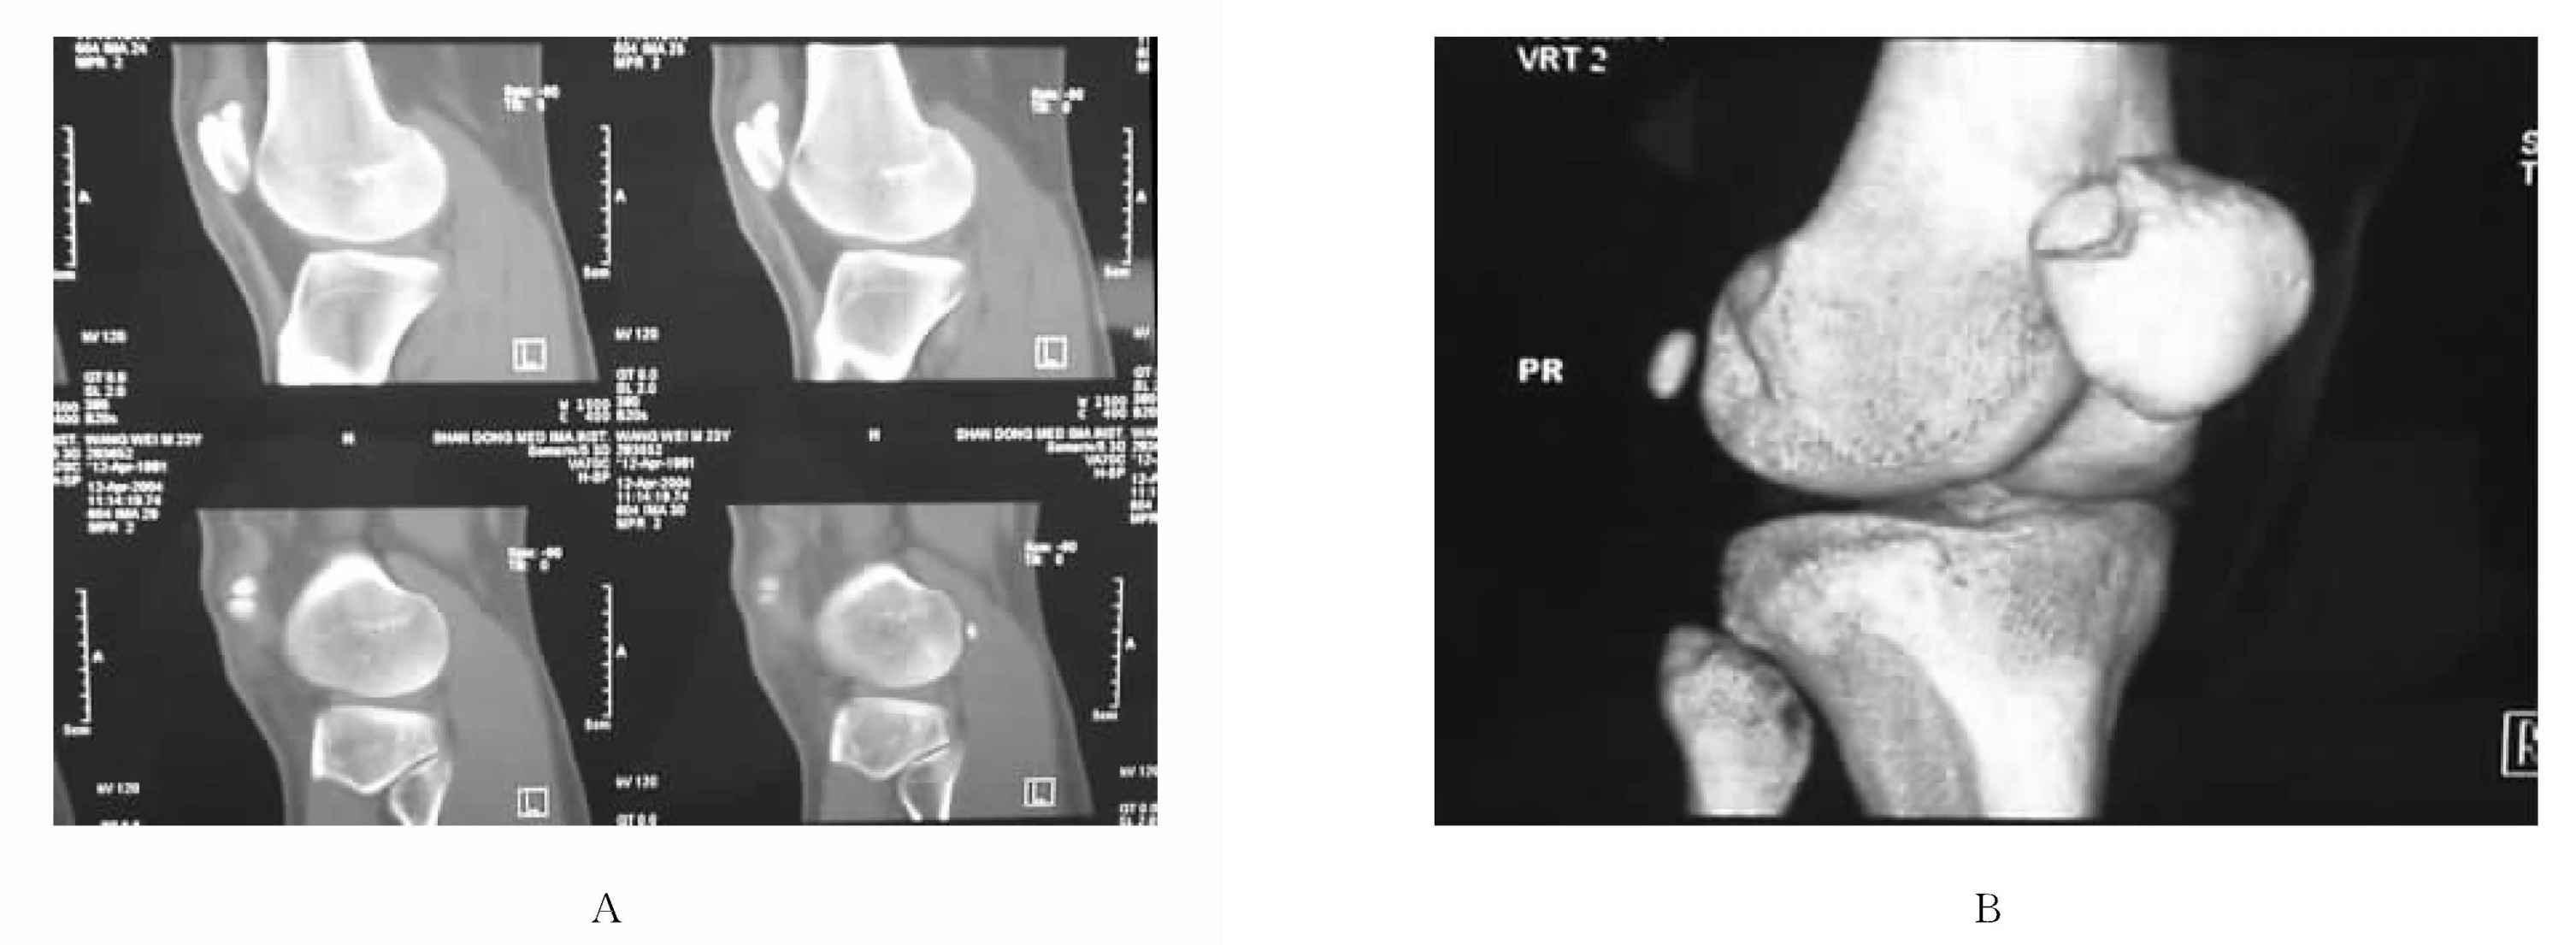
\includegraphics[width=.7\textwidth,height=\textheight,keepaspectratio]{./images/Image00417.jpg}
 \captionsetup{justification=centering}
 \caption{二分髌骨的多平面重建和三维重建}
 \label{fig22-1}
  \end{figure} 

\section{正常解剖和CT表现}

\subsection{肩关节}

肩关节由肩胛盂与肱骨头构成,又称为盂肱关节。

\textbf{【CT表现】}
轴位CT像表现:①紧邻肩胛骨后面的岗上肌和岗下肌。②肩胛骨前面是肩胛下肌,肩胛下肌的后下方是大圆肌和小圆肌。③肱二头肌和肱三头肌分别位于肱骨近端前、后方;三角肌围绕在肩关节的上外侧。④正常时肱骨头关节面中1/3与肩胛盂中1/3相关节,肱骨头表面的透明软骨呈光滑的弧线状。⑤在喙突平面肱骨头基本呈圆形,在喙突以下平面渐出现大、小结节,肱头外形不规则。大、小结节之间是肱二头肌长头。⑥肩胛盂关节面略凹,被覆的透明软骨中间薄、四周厚,周边演变为纤维软骨是盂唇,盂唇基本是三角形。⑦维持肩关节稳定的重要韧带包括肩袖、肱三头肌长头、肱二头肌长头。

\subsection{肘关节}

扫描方法:病人俯卧,将患肢上举,肘关节屈曲90°置于头顶上方,前臂中位(拇指向上)并与定位线平行。扫描范围从肱骨髁上至鹰嘴远端,以<5mm层厚和层距扫描,也可在肘关节伸直位时进行扫描。屈曲位扫描可清楚显示肱桡关节、肱尺关节。伸直位扫描可清楚显示肱骨远端及上尺桡关节。

\textbf{【CT表现】}
伸直位横断面图像示:①肱骨髁间平面:肱骨下端前后变扁,后缘偏内侧边缘微凹为肱骨滑车后关节面,它与其后的尺骨鹰嘴前面的关节面构成关节。鹰嘴的后缘显示肱三头肌腱。肱骨前面有肱肌,肱肌前为肱二头肌,内侧为旋前圆肌,这3块肌肉间隙内见肱动、静脉及正中神经。肱骨下端的内侧后缘可见尺神经。②尺骨冠突层面:冠突呈不规则形,外缘弧形凹面为桡切迹,它与圆形的桡骨头内缘之间有关节间隙。桡骨头外围有桡骨环状韧带,韧带的两头附着于冠突桡切迹的前、后缘。近侧桡尺关节的后面是肱三头肌,其外侧为桡侧腕长伸肌,后者的前方是肱桡肌。肱肌在尺、桡骨前,肱肌与肱桡肌之间有桡神经。肱肌前内方是旋前圆肌。肱肌前面是肱动、静脉和正中神经。冠突内侧有指浅屈肌和尺侧腕屈肌,它们与尺骨之间有尺神经。

\subsection{腕关节}

腕关节因解剖位置的关系,可行轴位、冠状位和矢状位三个方向的扫描。腕关节包括桡腕关节、腕中关节和掌腕关节3部分,以冠状位显示为佳。

1.桡腕关节:桡骨远端、尺骨的纤维性三角软骨盘与近排腕骨的舟状骨、月骨、三角骨构成桡腕关节。桡骨下端凹陷,容纳舟状骨和月骨。尺骨下端不直接参与桡腕关节。桡腕关节腔与下尺桡关节腔互不相通。

2.腕中关节:亦称腕骨间关节。由近排腕骨和远排腕骨构成,关节间隙呈S形。舟状骨、月骨构成凹形的尺侧半,容纳头骨近端。

3.腕掌关节:第2~5掌骨基底与远排腕骨构成第2~5掌腕关节。第1掌骨与大多角骨构成单独的拇指腕掌关节,与其他关节不通。

\textbf{【CT表现】}
远排腕骨横断层面显示远排腕骨沿手腕背侧面排列,呈凹向掌侧的弧线,大多角骨与钩骨相对,中间的空隙主要为腕管的断面。腕管内有指浅、深屈肌腱和拇长屈肌腱,共9条,正中神经位居前部。腕管和大多角骨前面为拇指对掌肌和拇短展肌。腕管正前方是掌腱膜,最内方为小指短展肌和小指对掌肌。手腕背侧亦有许多的深肌腱。

掌骨近端横断层面与远排腕骨层面相似,显示第1~5掌骨基底由内向外呈弓状依次排列,其掌侧为腕管的断面结构。

\subsection{髋关节}

髋关节由髂骨、耻骨、坐骨及股骨上端组成,股骨头与髋臼形成球窝形关节。

\subsubsection{儿童髋关节}

髋骨在成人是一块完整的不规则扁骨,在儿童有3个独立的骨块即髂、耻、坐骨所组成。胚胎时期这3骨各有1个初级骨化中心,出生后3者之间遗留1个Y形软骨,它实际是髂、耻、坐3骨共有的骺软骨。于8岁前后Y形软骨出现二次骨化中心。其闭合时间男性为16~17岁,女性为13~17岁。

股骨上端有3个骨骺,即股骨头骨骺和大小粗隆骨骺。

\textbf{【CT表现】}

儿童髋关节骨化过程呈以下CT表现:

4~5岁未骨化的Y形软骨,平片表现为髋臼顶波浪状钙化;CT可见到环形或斑点状钙化斑。8岁前后平片表现Y形软骨有多个二次骨化中心即小骨骺,Y形软骨偏上部骺板呈前后水平位;CT横断扫描可同时显示多个骨化中心。另外,Y形软骨的骨化带亦呈波浪状,故二者CT均可表现为环形钙化簇。

1.股骨头透亮环征:为股骨头骺与颈交界处的影像,中心密度高呈球形,外围可见透亮环,称为透亮环征。中心密度高的部分是网状紧密排列的骨小梁;外周透亮环为放射状纤细的骨小梁。环征由上往下逐渐变窄乃至消失,中心致密结构由模糊变清晰。

2.弧线征:为股骨头骨骺与干骺端之间形成的一透亮间隙,此透亮线为骺板软骨。此征在儿童髋关节半蛙式扫描时出现。

3.新月征:出现于较大儿童,因头骺增大,在股骨头的内侧面出现一个新月状骨骺。实际为头颈交界处的影像。

4.小凹征:位于头颈交界的前缘,呈0.5cm左右的圆形低密度,周围硬化,可单发或2~3个,其内无钙化。

此外,股骨大小粗隆可见多个骨化中心的不规则钙化,密度不均匀,勿误为骨折。

\textbf{【鉴别诊断】}

1.滑膜骨软骨瘤病:多见于30~50岁男性,多为单侧,钙化骨化位于关节腔内。而Y形软骨环形钙化发生于6~14岁,且为对称性,钙化斑位于髋臼顶的股骨头上缘。

2.髋臼缺血坏死:好发于青少年。常与股骨头缺血坏死和髋臼发育不良并存,多为单侧。影像学表现髋臼浅而宽,髋关节呈半脱位状态。髋臼密度不均,有囊变及周围硬化表现。股骨头骨骺变扁、增宽、囊变及破碎表现。

\subsubsection{股骨颈前倾角的测量}

小儿先天性髋关节脱位常需测量股骨颈前倾角。

\textbf{【测量方法】}
①患侧髋关节轴位扫描,并加扫股骨髁向后最突出层面。采用包括股骨颈图像层面和股骨髁最突出层面。②测量股骨颈中线与台面(水平面)角度(A)和股骨髁后缘连线与台面(水平面)所成角度(B)。③A角减去B角即为股骨颈前倾角(图\ref{fig22-2})。

\begin{figure}[!htbp]
 \centering
 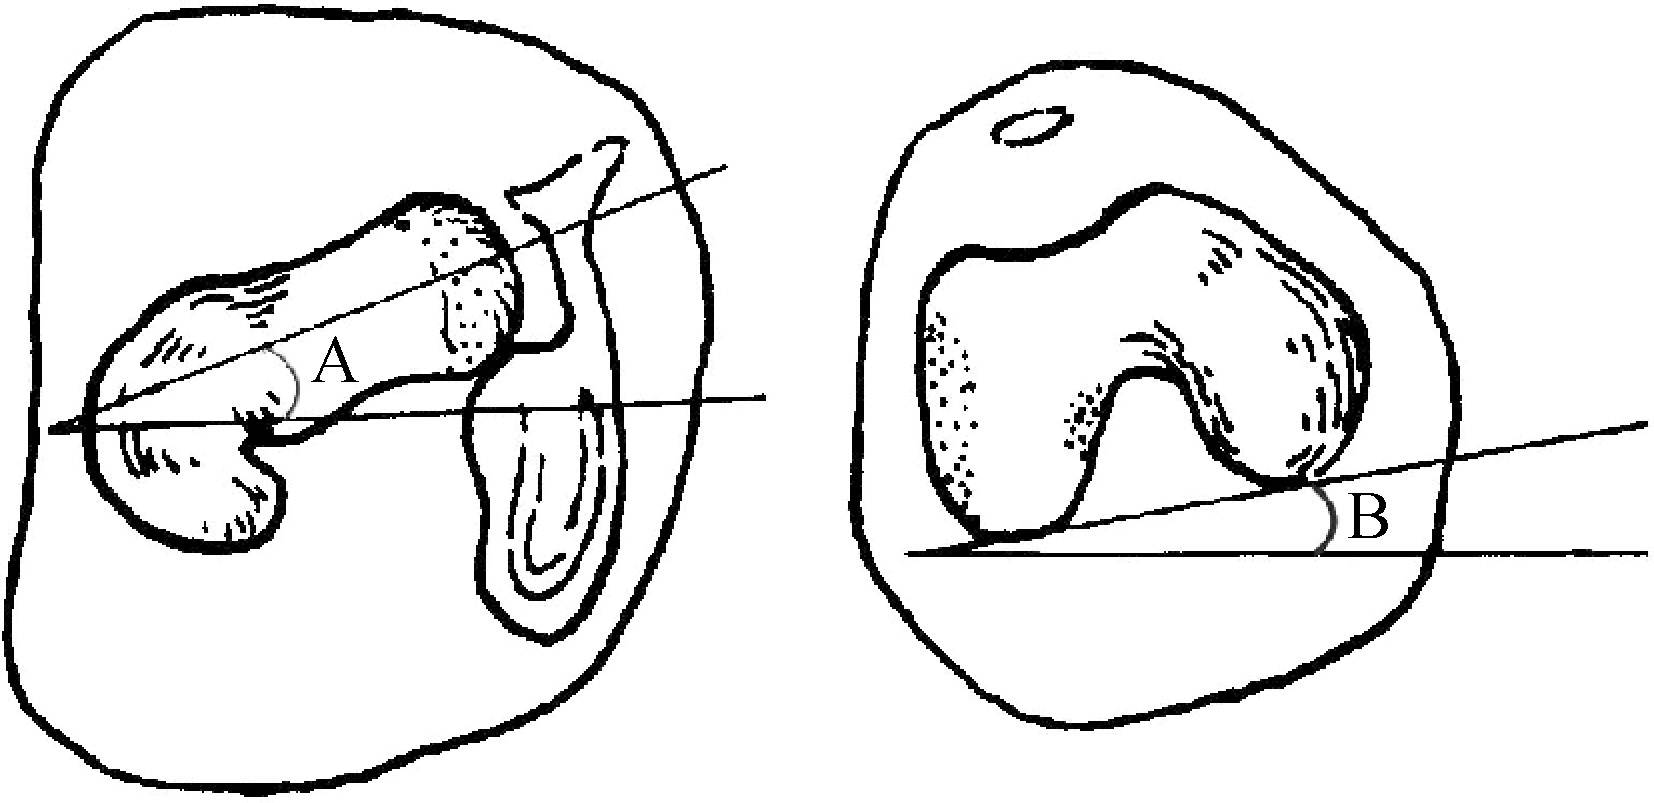
\includegraphics[width=.7\textwidth,height=\textheight,keepaspectratio]{./images/Image00418.jpg}
 \captionsetup{justification=centering}
 \caption{股骨前倾角的测量}
 \label{fig22-2}
  \end{figure} 

\subsubsection{髋臼的X线解剖}

髋臼是由髂、坐、耻3骨和体部共同组成的,分别是髋臼的上2/5、后下2/5及前下1/5。根据形态学和力学原理,又将髋臼分为两个柱和两个壁。前壁小于后壁,且较少发生骨折,后壁骨折则多见。①前柱(髂耻柱)始于耻骨支,经髋臼前内侧面向前延伸达髂前上棘或髂嵴。②后柱(髂坐柱)始于坐骨大切迹,经髋臼负重区和髋臼后面后方向下至坐骨结节。

X线平片其重要标志线:①髂耻线:是前柱内缘线,自坐骨大切迹外缘,向前沿骨盆边缘经耻骨上支至耻骨联合。②髂坐线:代表后柱外缘线,自坐骨大切迹垂直经髋臼的泪滴外侧延伸至闭孔下缘。③泪点线:用于判断髂坐线是否内移。④髋臼顶线:代表髋臼负重区。⑤前后缘线:髋臼前后壁的边缘线,需多体位摄片观察。⑥前柱线:又称髂耻柱线,代表前柱形态。⑦后柱线:又称髂坐柱线,代表后柱形态。

掌握以上X线解剖有利于正确认识髋臼的CT解剖。

\subsubsection{成人髋关节}

\textbf{【CT表现】}
髋臼中心层面示膨大球形的股骨头位于口朝外的半月形髋臼内。股骨颈前后缘见关节囊影,呈厚2~3mm的线条影,内侧分别附着于髋臼的前唇和后唇。大转子在关节囊外。股骨头边缘光滑,可见股骨头凹。在头的中央层面骨小梁粗大分散呈星芒状,叫星芒征。髋臼的骨盆缘覆以梭形闭孔内肌。髋臼后方有坐骨神经断面,再后是臀大肌影。髋关节前外侧有臀中肌、阔筋膜张肌、缝匠肌及紧贴关节深层的肌肉(髂腰肌、股直肌),前内方之股三角由外向内依次排列有股神经、股动脉、股静脉及其它们的分支。髋关节前关节间隙宽为0.2~0.4cm;后关节间隙宽0.2~0.3cm,中间关节间隙0.5~0.8cm。

\subsubsection{正常成人髋臼前倾角的测量}

\textbf{【测量方法】}
选择通过股骨头中心的层面作为赤道面。髋臼前后缘连线与双侧股骨头中心连线垂直线的外侧夹角即为髋臼前倾角。

\textbf{【正常值】}
国内有学者测量了100例正常成年人髋臼前倾角,并首次制定了其标准。国内男性正常范围为:6.51°~21.53°;女性的正常范围为:8.32°~25.38°。该数值较外国人稍低,可能与人种及测量误差有关。多数学者同意该角女性比男性大2°~5°。

\textbf{【临床价值】}
成人髋臼发育不良为较常见的疾病,尤其多见于女性,易早期发生髋关节退行性变并影响其关节功能,髋臼发育不良患者该角增大。结合其他表现,可早期诊断成人髋臼发育不良。

\subsection{骶髂关节}

1.正常成人骶髂关节的解剖特点和CT表现

其解剖特点为:①骶髂关节分为中下2/3的滑膜部和后上1/3的韧带部。②骶髂关节的外形变异很大,多数呈耳状,有的呈C形或钝角形。足月胎儿的骶髂关节面是光滑平整的,随年龄增加,关节内突起与凹陷增加并发生绞锁。③关节面表面覆有软骨,滑膜并不覆盖于关节软骨上,而是在关节软骨边缘与之融合。滑膜部关节软骨骶骨侧厚度为髂骨侧的2~3倍,其浅层为纤维软骨,深层为透明软骨;而髂骨侧的软骨只有纤维软骨构成,通常在1mm以下。也有文献认为,骶髂关节的软骨是透明软骨还是纤维软骨,还与年龄有关,一般年轻者均为透明软骨,随年龄增加就逐渐有纤维成分加入。

\textbf{【CT表现】}
①关节前下部有软骨和滑膜,关节间隙宽度一致,宽约2mm,关节面清晰锐利;后上部是韧带性的,关节间隙稍宽而不规则,关节面薄而不锐利。②儿童骶髂关节前、后两部无明显区别,关节间隙较宽,前后间隙宽窄一致,关节缘轮廓模糊。③左右髂骨面骨皮质基本对称,但前后不均,由前向后逐渐变薄。前部皮质厚度约16%可>5mm,95%滑膜关节中1/3处皮质厚度在2mm以上。髂骨面上中部前份关节面下骨皮质明显增厚,呈底在前的小三角形,密度均匀。④骶骨侧骨皮质均匀一致,边缘清楚,皮质厚度亦较薄,1~2mm者占62.5%。骶骨侧皮质的韧带附着处常不规则,酷似骨侵蚀。⑤由于部分容积效应,关节面有时不清晰,多见于髂侧滑膜部与韧带部移行区。

2.正常青少年骶髂关节的CT解剖特点

正常青少年骶髂关节的几种表现易误为骶髂关节炎(与AS的鉴别见本章第七节),如骶骨骨骺、关节面的局限凹陷、髂骨侧关节面的囊样改变及骶骨侧关节面的侵蚀样改变。骶骨骨骺均位于骶髂关节的骶骨侧,一般呈三角形、类圆形骨块影,但有时不规则,有节裂,呈条状、碎片状。骨骺处关节面亦可有明显凹陷。总之,骶骨侧关节面出现骨骺、骶骨分节处及骶骨前上缘骶骨侧关节面的局限性凹陷是正常青少年骶髂关节的特点,真空现象的存在不能作为病变的征象(有人认为正常青少年出现积气,可能是检查时关节受牵拉关节腔形成负压氧气游离出来所致)。

\subsection{骨盆}

骨盆由髋骨和骶、尾骨组成。髋骨上部为髂骨,前下部为耻骨,后下部为坐骨,它们借助两个滑膜关节(即左右骶髂关节)和两个纤维软骨性联合(即耻骨联合与骶尾联合)及一些韧带相互连结而成。

\textbf{【CT表现】}
CT可很好的呈示髂骨、耻骨和坐骨的体部、上支和下支,其中髂骨翼中央菲薄,轴位像仅见由两层皮质构成,无松质骨。

\subsection{膝关节}

膝关节由股骨和胫骨的内外侧髁及髌骨组成,上胫腓关节不参与膝关节构成。

\textbf{【CT表现】}

1.髌骨下部伸膝层面:股骨内、外侧髁在前部相连呈马蹄形,前面凹陷,形成一个凹面向前的股骨髁间沟角,且与髌骨的凸面关节面构成髌股关节。后面有大而深的髁间窝,窝内的外侧髁内面有前交叉韧带断面,内侧髁外面有后交叉韧带。外侧髁的外缘有腓侧副韧带,内侧髁的内缘有胫侧副韧带。股骨髁的后方中央偏外侧有股动、静脉及胫神经,依次由前向后排列,它们的两旁为腓肠肌内、外侧头。外侧髁后缘是跖肌,内侧髁后方有半腱肌、半膜肌及缝匠肌。

2.膝关节中部伸膝层面:最前方是髌韧带、髌下脂肪垫,其后为胫骨髁关节面上的内、外侧半月板。两个半月板之间,是内、外侧髁间隆起的断面。内侧半月板的内侧有胫侧副韧带,外侧半月板的外侧有腓侧副韧带及股二头肌腱。

\subsection{踝部及足部}

主要解剖结构有:①踝关节由胫骨、腓骨下端及距骨滑车组成。距骨分为距骨头、颈、体3部分。距骨头关节面与舟骨构成距舟关节;体部上面为滑车;体部下方有前、中、后3个关节面,前、中关节面参与构成距跟舟关节,后关节面与跟骨关节面构成距跟关节,二者被跗骨管分开。②跗横关节由距舟和跟骰两关节合成。

\textbf{【CT表现】}

1.踝关节层面:显示居中的距骨上关节面,内、外两侧的内踝和外踝,以及距骨与内、外踝之间的踝关节内、外两侧方关节间隙。

2.跟距关节层面:显示前方的距骨和后方的跟骨以及两者之间的跟距关节。跟距关节由前内的支柱关节和后外的距下关节组成,前者较短小,呈水平走向;后者较宽大,呈斜行走向。

3.跖跗关节层面:显示第1~5跖骨基底由内向外下依次排开,呈“八”字排列,背面隆起,跖面凹陷,与腕管相似,内含屈趾肌腱、神经和血管。

此外,在CT图像上,肌腱呈边界清楚、圆形、密度均匀影,CT值比肌肉高,被周围脂肪组织清晰衬托。

\subsection{脊柱}

1.椎骨:由椎体和椎弓(习惯称为附件)构成,椎弓包括椎弓根、椎板、横突、关节突和棘突。椎体的横断面自上向下增大,颈椎体扁长,胸椎体近似圆形,后面凹形;腰椎体呈椭圆形。颈椎体侧缘有钩椎关节且关节面有软骨覆盖。

2.椎管:由椎孔连接而成,椎体、椎弓根和椎板围成椎管的骨环。椎管前壁为椎体、椎间盘后面及其表面的后纵韧带,后壁为椎板和黄韧带,侧壁为椎弓根内面和椎间孔。在CT轴位像上颈椎椎管为三角形;胸椎近圆形;腰上段为椭圆形,腰下段为三叶形;而在新生儿腰椎管全为椭圆形。由于胸椎椎板向后下方倾斜呈叠瓦状,因而在一个层面上可见到上、下两个椎体的椎板。

3.椎间小关节:由上、下关节突组成,在轴位CT图像上,左右关节面对称。①颈椎椎间关节间隙方向与水平面平均成45°角,下颈椎关节面趋于水平。②胸段椎间关节方向与水平面成60°角,与冠状面平行。③腰椎椎间关节方向与水平面成90°角,关节间隙由上至下由矢状位渐趋于冠状位。

\section{骨与关节创伤}

\subsection{肩关节骨折和脱位}

1.肩胛骨骨折:按部位可分为关节盂或关节面骨折、肩胛颈骨折、肩胛体骨折、肩胛冈骨折、肩峰骨折和喙突骨折,其中肩胛体骨折最常见,CT可予明确显示(图\ref{fig22-3})。

\begin{figure}[!htbp]
 \centering
 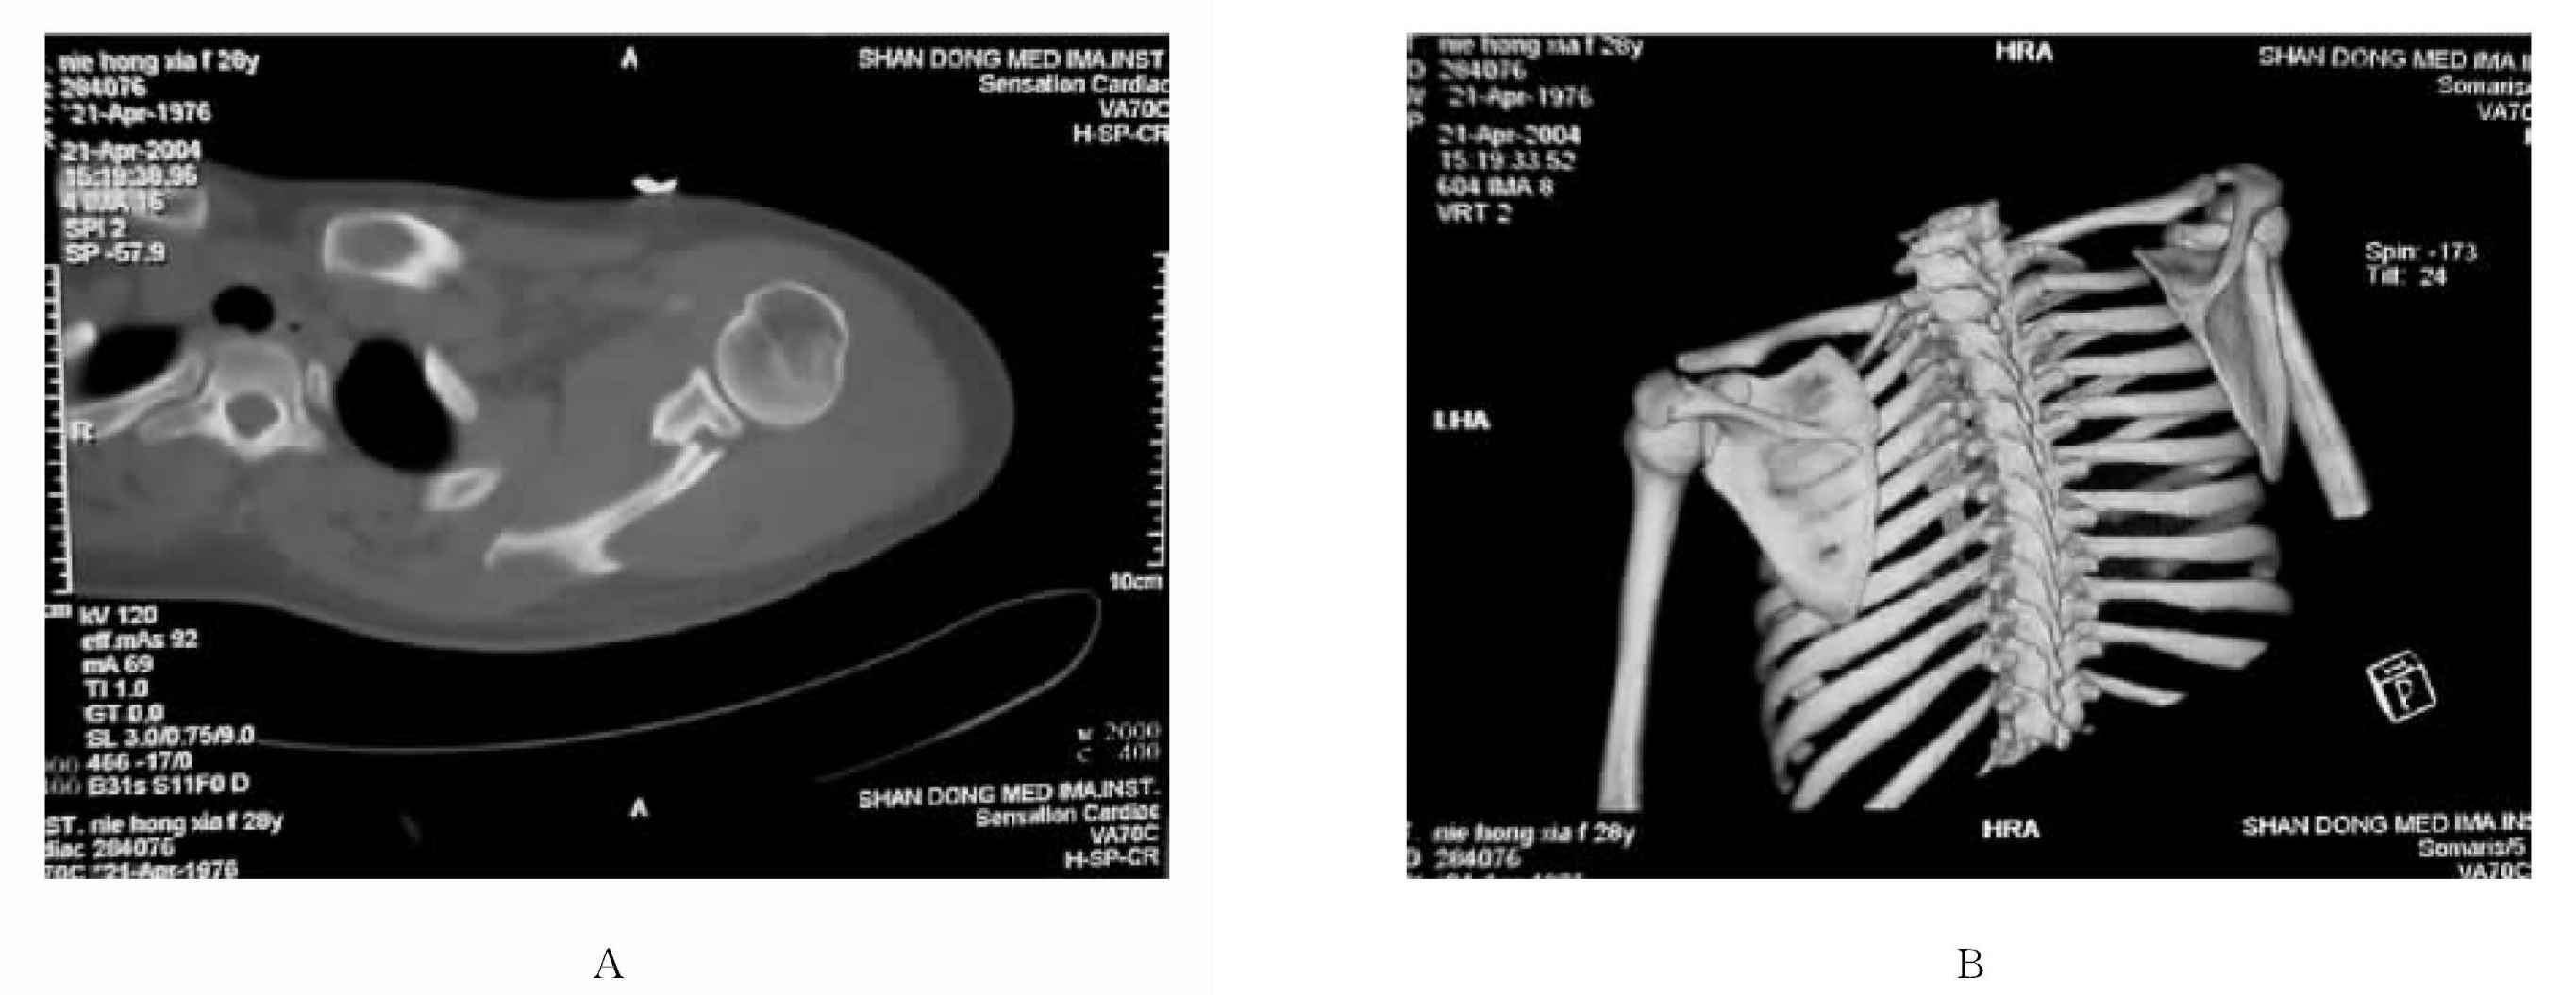
\includegraphics[width=.7\textwidth,height=\textheight,keepaspectratio]{./images/Image00419.jpg}
 \captionsetup{justification=centering}
 \caption{左侧肩胛骨骨折\\{\small A、B为同一患者}}
 \label{fig22-3}
  \end{figure} 

2.肱骨近端骨折:CT能很好的显示肱骨头、大结节、小结节、肱骨干上段的骨折及其移位的程度。

3.肩关节脱位:分为前脱位、后脱位、上脱位和下脱位4型,其中前脱位最常见,约占肩关节脱位的95%。CT能予以明确显示,并清楚地显示关节面的损伤、关节内碎骨片、X线片易于漏诊的后脱位等。①在CT上如果肱骨头关节面的中1/3不与肩胛盂的中1/3相对应,可诊断为肩关节脱位。②肩关节前脱位时,肱骨头后外侧撞击肩盂前缘,导致肱骨头后外缘V形骨折,称为希尔-萨克斯(Hill-Sachs)损伤。③前脱位时还可伴肩盂前下缘骨折或盂唇软骨的撕脱骨折,称为班克特(Bankart)损伤,是复发性肩关节脱位的主要原因。④肩关节后脱位合并肱骨头内侧缘撞击肩盂,导致肱骨头内侧骨折,在轴位图像中呈“Thoughline”现象。

\subsection{肘关节骨折和脱位}

1.肱骨远端骨折:①髁上骨折;②经髁骨折;③髁间骨折;④髁部骨折(内髁或外髁);⑤关节面骨折(肱骨小头和滑车);⑥内上髁骨折。

2.尺骨近端骨折:有鹰嘴骨折和冠突骨折。单纯冠突骨折少见,常伴肘关节后脱位,而肘关节前脱位常并鹰嘴骨折。

3.桡骨近端骨折:可分为桡骨头骨折和桡骨颈骨折。

CT扫描可显示相应骨折线、骨折片、移位程度及有无关节脱位等。

\subsection{腕关节骨折和脱位}

CT检查常用于显示复杂的腕骨骨折、不易显示的骨折、关节面受累与否、骨折愈合情况判断、下尺桡关节脱位以及软组织异常。

1.舟状骨骨折:是腕部最常见的骨折,可分为5类:近端骨折、腰部骨折、远端骨折、结节骨折、远端关节面骨折。诊断时应注意:①如果一侧骨皮质中断而骨小梁并无中断则可能是滋养动脉孔。②陈旧性舟状骨骨折远端骨质疏松,近端骨质硬化或出现囊变,提示缺血坏死可能。

2.钩骨骨折:最常见的是钩突部骨折,X线平片难以显示。CT可予明确显示,并可显示骨折片移位程度,以及腕管的扩大或缩小。

3.下尺桡关节脱位:是指尺骨向背侧或掌侧移位,以背侧半脱位最常见,平片常难以诊断,而进行旋前位、中立位和旋后位CT扫描对比观察可予明确诊断。

\subsection{髋臼骨折}

髋臼骨折的分类方法很多,目前国际公认分为10类:①前柱骨折;②后柱骨折;③双柱骨折;④前柱伴后半横行骨折;⑤后柱伴后壁骨折;⑥前壁骨折;⑦后壁骨折;⑧横行伴后壁骨折;⑨横行骨折:髋骨在髋臼部被横断分离为上方的髂骨和下方的坐耻骨;⑩“T”型骨折:横行骨折合并远折段的纵行骨折,后者骨折线经臼内侧壁向远侧延伸,可累及闭孔环。

CT对于髋臼骨折的分类意义有限。大多数学者认为CT检查的作用次于X线平片,CT的价值是提供骨折移位、旋转情况和关节、股骨头形态。

\subsection{髋关节脱位}

外伤性髋关节脱位可分为:①后脱位;②前脱位;③中心脱位;④半脱位;⑤双侧脱位;⑥外侧脱位;⑦陈旧性脱位。一般X线平片都能诊断。

CT检查的目的是为了确定髋臼和股骨头有无骨折及骨折块所在的位置,即是否位于关节内而阻碍复位;评价关节面的完整性及复位后股骨头的稳定性。对中心性髋关节脱位可评估骨盆口的大小及形状,对年轻生育女性的产道评估有重要意义。此外,由于关节内骨折,血液及髓内脂肪进入关节囊,形成关节脂血征(此征亦可见于其他关节内骨折;图\ref{fig22-4});如另有气体进入被称为关节积气脂血征,此征象对诊断关节内骨折甚有意义。

\begin{figure}[!htbp]
 \centering
 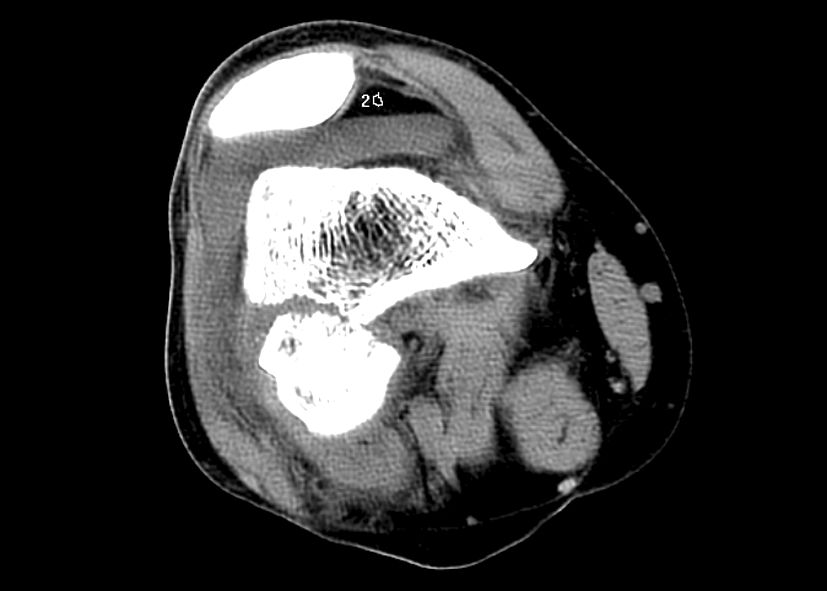
\includegraphics[width=.7\textwidth,height=\textheight,keepaspectratio]{./images/Image00420.jpg}
 \captionsetup{justification=centering}
 \caption{股骨远端骨折并膝关节内脂血征\\{\small 膝关节腔内有脂-血平面}}
 \label{fig22-4}
  \end{figure} 

\subsection{骨盆骨折}

骨盆骨折可分为4型。Ⅰ型:无损于骨盆环完整性的骨折,如髂骨翼骨折、撕脱骨折、单一耻骨支或坐骨支骨折;Ⅱ型:骨盆环一处骨折,如一侧耻骨上下支骨折、骶髂关节半脱位、耻骨联合分离;Ⅲ型:骨盆环两处以上骨折,如双侧耻骨上下支骨折、骨盆环前后联合损伤;Ⅳ型:髋臼骨折。Ⅰ型常是稳定骨折,其他为不稳定骨折。

国外有学者认为,以下损伤时应做CT检查:①骨盆环双侧垂直骨折脱位,一般X线平片难以正确判断骨盆的稳定性。②骨盆环骨折涉及髋臼。③半骨盆较重损伤考虑内固定治疗的。此外,单纯Ⅰ型骨折累及关节者亦常需CT检查。

\subsection{胫骨平台骨折}

其分类方法很多,可分为以下6型。Ⅰ型:单纯劈裂骨折;Ⅱ型:劈裂塌陷骨折;Ⅲ型:单纯中央塌陷骨折;Ⅳ型:内侧髁骨折;Ⅴ型:内外侧髁骨折;Ⅵ型:伴有干骺端和骨干分离的平台骨折。

对骨折评估来说,确认关节面塌陷的形状和程度非常必要,而常规X线平片对骨折粉碎程度估计不足;对塌陷程度测量不够准确,对平台前方及中心部位的塌陷估计过少,对后部塌陷往往估计过多。CT扫描则可补充X线平片所见,并准确估计和测量。

\subsection{髌股关节脱位}

髌股关节半脱位(关节紊乱)常规X线平片极难诊断,CT扫描可予准确的测量诊断。扫描时患者仰位,双膝伸直,以5mm层厚和层距扫描,取髌骨中央层面测量。

1.股骨髁间沟角:内外髁最高点与髁间沟最低点连线所成的夹角,正常值为142°角,范围从129°~150°,大于此值为髌股脱位(图\ref{fig22-5})。

\begin{figure}[!htbp]
 \centering
 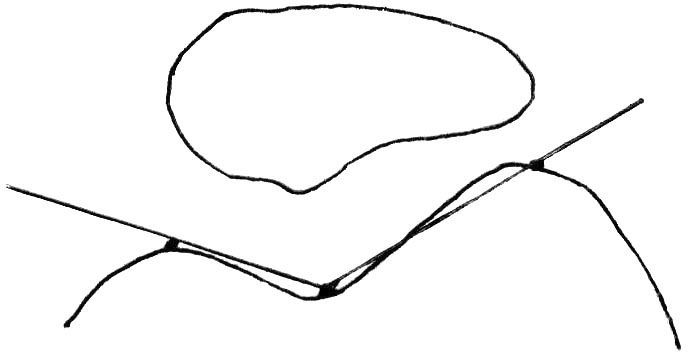
\includegraphics[width=.7\textwidth,height=\textheight,keepaspectratio]{./images/Image00421.jpg}
 \captionsetup{justification=centering}
 \caption{股骨髁间沟角的测量}
 \label{fig22-5}
  \end{figure} 

2.适合角:先平分股骨髁间沟角,髌骨最低图像点与股骨髁间沟最低点连线与股骨髁间沟角平分线的夹角为适合角。平分线外侧为正,内侧为负。正常平均角度为-6°,>16°为异常(图\ref{fig22-6})。

\begin{figure}[!htbp]
 \centering
 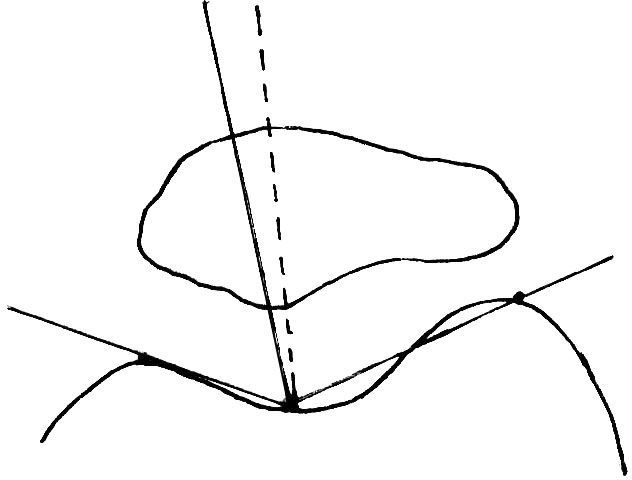
\includegraphics[width=.7\textwidth,height=\textheight,keepaspectratio]{./images/Image00422.jpg}
 \captionsetup{justification=centering}
 \caption{适合角的测量\\{\small 实线为髌和股骨髁间沟最低点连线;虚线为髁间沟角平分线}}
 \label{fig22-6}
  \end{figure} 

3.外侧髌股角:内外髁最高点连线与髌骨外侧关节面切线所成的夹角。此角正常开口向外侧,但有30%为平行线。髌骨脱位者开口向内或平行(图\ref{fig22-7})。

\begin{figure}[!htbp]
 \centering
 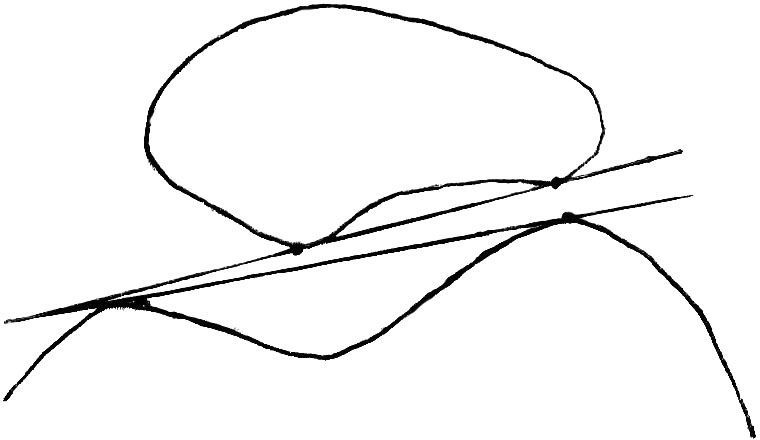
\includegraphics[width=.7\textwidth,height=\textheight,keepaspectratio]{./images/Image00423.jpg}
 \captionsetup{justification=centering}
 \caption{外侧髌股角的测量}
 \label{fig22-7}
  \end{figure} 

\subsection{跟骨及踝关节骨折}

1.跟骨骨折:很常见,约75%累及距下关节。CT扫描能清楚地显示骨折块大小、数目、骨折移位、粉碎程度、关节面受累情况。跟骨后关节面在冠状位显示最好,并可确定有无关节面塌陷,且可在冠状面上显示内侧拇长屈肌腱和外侧腓骨长、短肌腱,跟骨骨折后常撞击这两条肌腱,造成肌腱炎,导致慢性足疼。有学者报道92%的跟骨骨折病人有腓骨肌腱的异常。

2.踝关节骨折:主要依靠X线平片,但特殊骨折需CT扫描协助,例如可精确判断三踝骨折之后踝骨折片大小及粉碎程度。

此外,肌腱部分断裂表现为肌腱周径增大,肌腱内有透明区。

\subsection{寰椎爆裂骨折和寰枢关节半脱位}

1.寰椎爆裂骨折:由垂直暴力产生,使寰椎前后弓骨折,双侧侧块分离移位。CT可精确测量寰椎侧块移位的程度,判断骨折的稳定性。测量方法为:在寰椎平面测量移位侧块间的距离,在枢椎平面测量枢椎关节面外缘之间的距离,如果前者超过后者7mm以上,说明寰椎之横韧带断裂,骨折不稳定;若差值<7mm,可以认为骨折稳定。

2.寰枢关节半脱位:齿突前缘和寰椎前弓后缘的正常平均距离在成人中为2mm,儿童为5mm,此间距增大即表示存在半脱位。常由寰椎横韧带断裂或其附着部位撕脱骨折引起。单独寰椎横韧带撕裂可致寰椎移位5mm;>5mm的位移则提示翼状韧带等结构的损伤;位移>10mm的则寰枢之间的一切韧带都断裂,脊髓必然受压。但寰椎横韧带撕裂导致的此间距增宽在颈椎前屈时最显著,而CT扫描是在中立位或后伸位进行的,影响了其诊断灵敏度。

\subsection{寰枢椎旋转性半脱位}

本病又称寰枢椎旋转固定,是指寰椎和枢椎在一个旋转半脱位位置上持续固定状态,使寰椎和枢椎作为一个单元而参与运动。共分为4型:Ⅰ型:横韧带完整,寰椎侧块以齿突为旋转中心,一侧向前旋转移位,一侧向后旋转移位;Ⅱ型:横韧带断裂,以一侧寰枢关节为旋转中心,另一侧侧块向前旋转移位;Ⅲ型:为Ⅱ型的加重状态,齿突前缘与寰椎前弓后缘的距离大于5mm;Ⅳ型:一侧寰椎侧块向后旋转移位,常伴齿突骨折。

轴位CT图像可见齿突与侧块之间的解剖位置关系异常,连续两个层面所显示的侧块移位程度不同。但是齿突与寰椎两侧块间距离轻度不等,可以是正常变异,不能作为寰椎脱位的依据。诊断寰枢椎旋转固定的最好方法是在颈椎中立位及头部向对侧最大旋转位两个位置进行轴位CT扫描。

\subsection{颈椎小关节半脱位}

其脱位可分为两侧和单侧。

1.两侧小关节脱位:由颈椎屈曲损伤造成,属不稳定型。

\textbf{【CT表现】}
在轴位CT图像上,脱位的小关节产生“小关节裸征”,上、下关节突的关节面不再对应,可见上关节突呈半月形,显露出平坦的后部关节面。

2.单侧脱位:由颈椎屈曲旋转损伤造成,最常见于C\textsubscript{5}
、C\textsubscript{6}
。单纯脱位是稳定的,而伴有神经损伤或关节面骨折的脱位则是不稳定的。

\textbf{【CT表现】}
在轴位CT图像上,即可见“小关节裸征”,又可见“背对背半月征”。后者即上下关节突“背部”(关节面的相对面)互相接触,而平坦的关节面构成了前后边界。

此外,无论单侧还是双侧关节损伤,还可表现为关节间隙增宽、关节积血、关节柱不对称、钩椎关节顺列异常等。

\subsection{脊柱骨折和脱位}

Denis将脊柱分为前、中、后三柱。①前柱由前纵韧带及椎体和椎间盘前2/3组成;②中柱为椎体和椎间盘的后1/3及后纵韧带组成;③后柱由椎弓及其附件、黄韧带、棘间韧带、棘上韧带组成。三柱中,中后柱是极为重要的,并把不稳定骨折规定为中、后柱脊柱断裂。

1.脊柱骨折的基本影像学征象

基本征象如下:①椎体压缩骨折:椎体前缘和侧缘皮质皱折、中断、嵌入、局限性隆起;椎体出现骨小梁中断、致密压缩带、椎体前上角骨片等。不能将椎体的单纯楔形变作为椎体压缩骨折的依据。②椎弓骨折。③关节突骨折。④椎板骨折。⑤横突骨折。⑥棘突骨折。⑦单纯环椎骨折少见,多伴有齿状突骨折。⑧椎轴成角(可X线平片、CT定位像或矢状重建观察)。

2.不稳定骨折

国外有学者提出不稳定骨折的4个放射学特征:①脱位;②椎板间隙增宽;③椎体骨突关节间隙增宽;④椎管增宽(椎弓根间距增宽)。

还有文献阐明临床常依以下3点判断脊柱失稳:①损伤累及三柱中的两柱或两柱以上;②骨性椎管变形狭窄;③骨折脱位和(或)较严重的后突畸形。

国外还有学者将椎管狭窄的程度分为3度:即椎管狭窄1/3为轻度、2/3为中度、2/3以上为重度。

3.脊椎爆裂性骨折

脊椎爆裂性骨折是压缩性骨折的一种特殊形式,是脊椎遭受垂直轴向压力,加上不同程度的前屈力,髓核向下位椎体内突入,导致下位椎体的爆裂而引起的椎体粉碎性骨折。占脊柱骨折的18.8%。绝大多数发生于T\textsubscript{9}
~L\textsubscript{5} 椎节,其中L\textsubscript{1}
占半数。骨折分类时,以中柱或椎体后缘是否受累来确定是单纯压缩型或爆裂型骨折。前者累及中柱的一部分而不累及椎体后壁,后者骨折线通过椎体后壁。

CT表现:①向心性椎体粉碎,后移骨片绝大多数均来自椎体的后上角。②椎体后壁骨折片向椎管内移位,导致椎管不同程度的狭窄。后移骨片以单个中央骨片居多,偶尔可见分离的骨片旋转移位。③半数病例可见椎体下部矢状方向骨折线,从基底静脉伸入到椎体前部。④后柱受累最多见的是一侧或两侧椎板垂直方向骨折。⑤其他伴随骨折有棘突、横突、椎弓根、关节突的骨折及小关节半脱位(图\ref{fig22-8})。

\begin{figure}[!htbp]
 \centering
 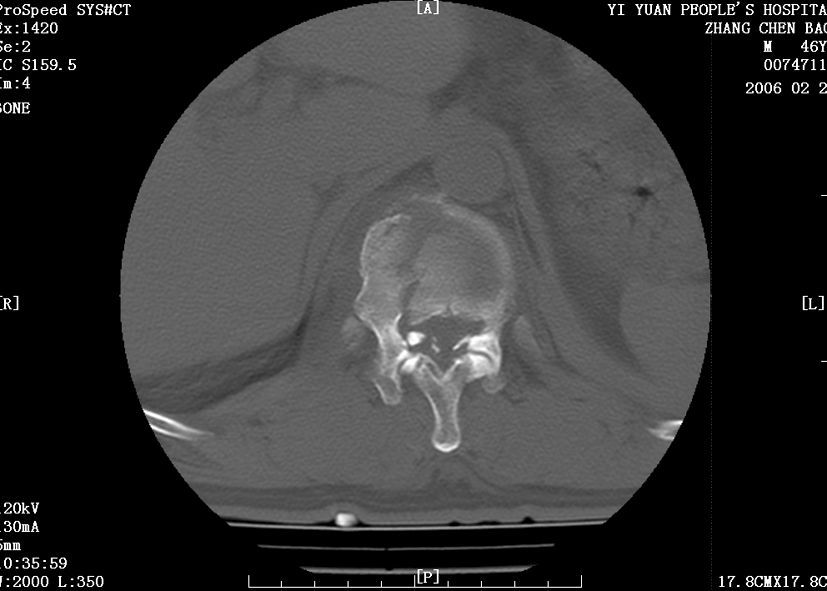
\includegraphics[width=.7\textwidth,height=\textheight,keepaspectratio]{./images/Image00424.jpg}
 \captionsetup{justification=centering}
 \caption{胸椎爆裂骨折\\{\small 椎体后上缘有后移骨片;关节突骨折及右侧小关节半脱位}}
 \label{fig22-8}
  \end{figure} 

此外,国外有学者发现所有爆裂骨折均有后壁骨折片突入椎管,平均椎管受压40%~60%,而伴神经损伤发生率为20%~40%,亦有学者报道椎管受压超过50%者或严重骨折脱位无神经损伤者并非罕见。但椎管受压越严重、骨折部位越高,发生神经损伤的可能性就越大。

4.老年性骨质疏松脊椎骨折与转移瘤性骨折

(1)老年性骨质疏松:①所有椎体都有骨质疏松,表现为椎体上、下面骨板密度相对增高。②压缩变形的椎体上、下面亦表现相对密度增高,而且是完整的。椎体皮质亦是完整的,随诊无椎体破坏。③椎旁无软组织肿块,但在椎体周围可出现薄环状或厚环状软组织影。有学者报道薄环状90%为良性;厚环状(>1cm)可为良性或恶性;肿块状为恶性。④压缩的椎体内出现真空现象,位于椎板下,呈线形,多认为是椎体缺血坏死的特征性表现,此征基本可排除恶性。⑤压缩的椎体上下骨板全部凹陷呈双凹征是良性病变的特征。⑥椎体后缘向后成角突出。

(2)转移瘤:与良性骨折相反。①唯独被压缩的椎体密度减低,有的发生明确的骨质破坏。②椎体上下面和四周骨皮质总有破坏消失之处。骨质破坏常累及椎弓根,椎弓根呈膨胀性改变是诊断恶性椎体压缩骨折的特异征象。③椎体周围出现半球形或非对称性软组织肿块,多不超过病椎上下椎体。但亦可无明显软组织肿块。④椎体上面或下面骨板呈弥漫性或局限性成角性凹陷或半圆形凹陷时,以恶性病变可能大。⑤椎体后缘向后呈球形突出。

\subsection{应力性骨折}

所谓应力性骨折是指肌肉运动作用于不能与之相适应的骨骼,无外伤而产生的骨折。分为疲劳性骨折和功能不全性骨折(亦称为衰竭性骨折)两大类。

1.疲劳性骨折

系因应力和肌肉力已超过了骨的正常弹性限度而引起的慢性骨折。常见病因为持续外力或长期积累性损伤如长期负重、跳跃、行军、跑步等。临床表现为局部疼痛和肿胀。

\textbf{【病理】}
骨小梁的断裂与新骨的增生同时进行。好发于第2、第3跖骨及胫骨,股骨、尺桡骨、肋骨、胸腰椎、跟骨等亦可发生。

\textbf{【影像学表现】}
骨折线大部呈横行、完全性或不完全性。大的管状骨骨折线常发生于一侧骨皮质。骨折线多不明显,而表现为边缘模糊的横行带状密度增高影。骨折线周围有骨膜反应、皮质增厚及髓腔硬化。

2.功能不全性骨折

又称衰竭性骨折,即为正常范围内应力作用于缺乏弹性的骨骼所致。常见病因为骨质疏松(老年性、闭经后、酒精中毒和大量皮质激素治疗后),其他还有类风湿性关节炎、放疗、关节置换、急性骨折和肢体废用,骨肉瘤术后等。典型症状为活动后加重、休息后缓解的患部疼痛。

\textbf{【病理】}
微骨折多首先发生于松质骨,骨小梁塌陷。3~4周后开始修复,可见病变区骨小梁聚集,内骨痂形成或骨内、骨周新生骨形成,并可出现骨坏死、骨髓出血、骨髓纤维化等。易发生于身体承重区或非承重区易受扭曲力作用的部位如骶骨、髂骨、耻骨、坐骨、髋臼、股骨颈及距骨等,且常双侧发病,有文献报道以骶髂关节(包括骶骨和髂骨)最常见。

\textbf{【影像学表现】}
根据累及部位可分为:①皮质骨型:主要累及长骨骨干,呈线样密度减低区或骨膜新生骨形成,断端一般不产生移位或成角畸形(图\ref{fig22-9});②松质骨型:累及长骨端、椎体、骶骨等部位。由于松质骨压缩、骨小梁嵌入重叠以及内骨痂形成,骨折线呈带状硬化。如在骶骨可见一侧或双侧骶骨翼松质骨内垂直硬化带,椎体则呈环状硬化带。可有软组织肿胀,厚度<10mm,但无软组织肿块。

\begin{figure}[!htbp]
 \centering
 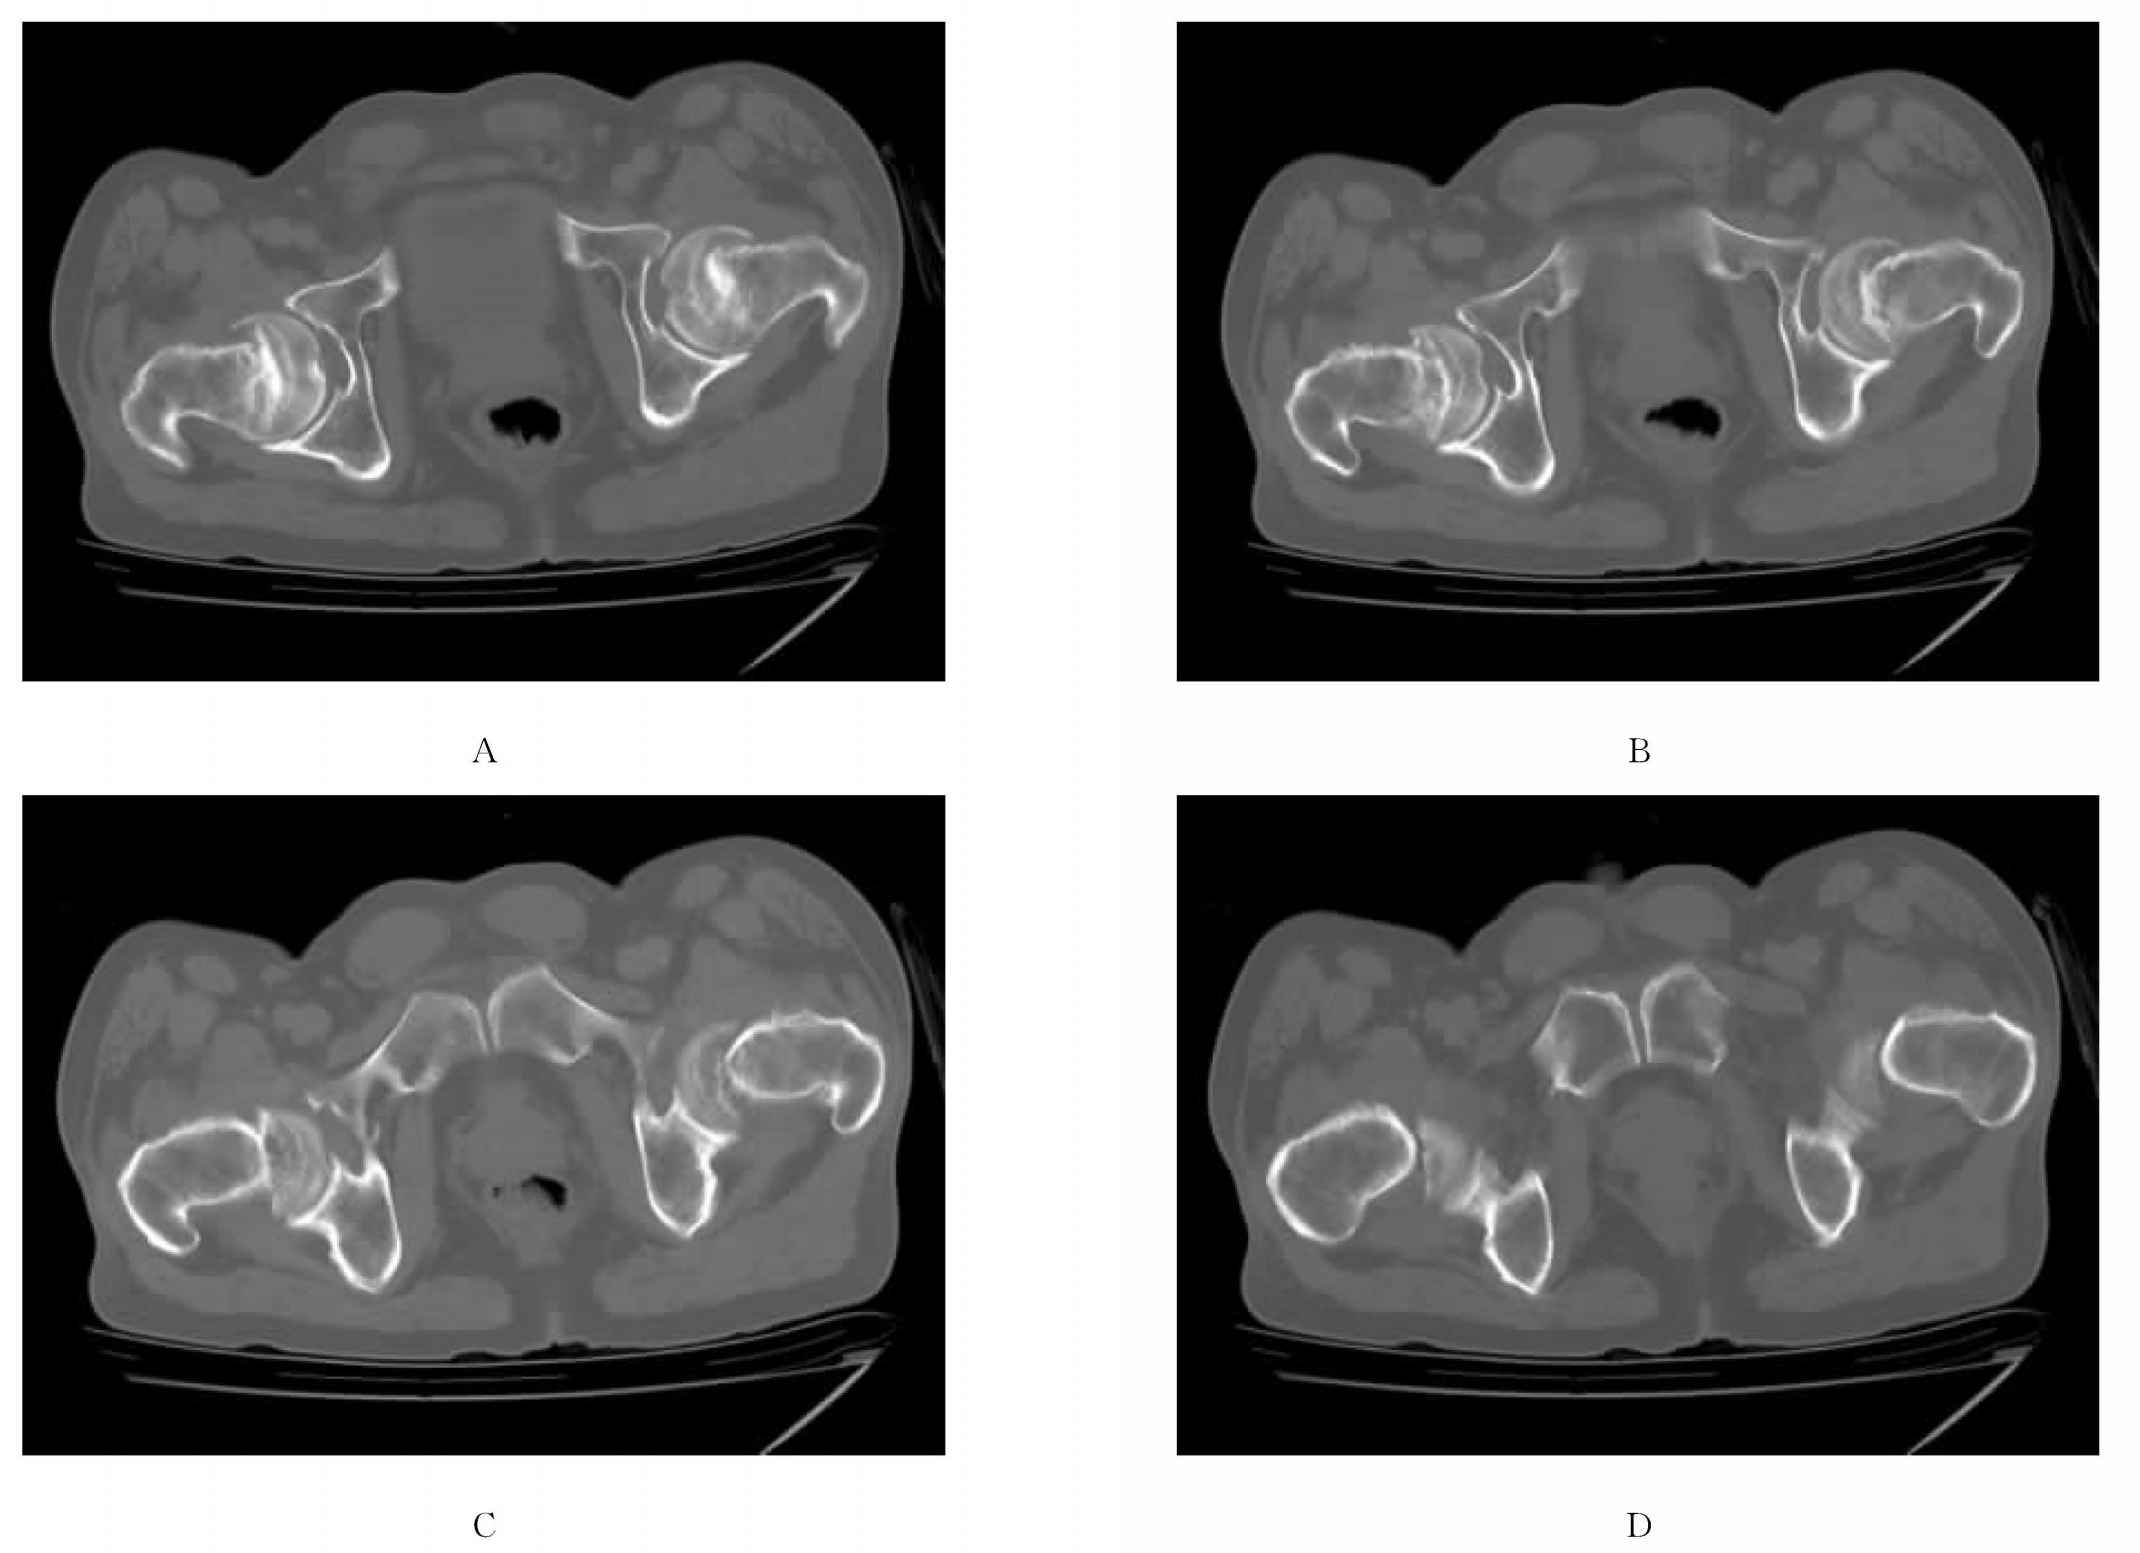
\includegraphics[width=.7\textwidth,height=\textheight,keepaspectratio]{./images/Image00425.jpg}
 \captionsetup{justification=centering}
 \caption{衰竭性骨折\\{\small A~D为同一患者,左右侧股骨颈部有线样低密度带,边缘硬化(无骨质软化症)}}
 \label{fig22-9}
  \end{figure} 

\section{骨关节感染}

\subsection{化脓性骨髓炎}

本病系指骨骼全部组织发生化脓性感染,包括骨炎、骨髓炎及骨膜炎。

\textbf{【病因病理】}
致病菌以金黄色葡萄球菌最常见。感染途径以血行最常见,亦可邻近软组织感染蔓延或经伤口引起。

病变常起始于干骺端骨松质内。感染后24小时至10天间无明显骨质破坏,最早仅有软组织及髓腔内充血、炎性水肿。此后,破骨细胞沿哈氏管及伏克蔓氏管浸润吸收产生细微的骨质破坏。第10天后骨质破坏逐渐明显,脓肿形成。随着病情进展,脓肿可穿破骨皮质到骨膜下形成骨膜下脓肿;亦可沿骨髓腔蔓延至骨干形成多个脓肿,然后穿破骨皮质沿骨膜下形成骨膜下脓肿。以上骨膜下脓肿均可经哈佛氏系统又回骨髓腔,亦可穿破骨膜形成软组织脓肿后破溃成窦道。少数干骺端的脓肿可穿破关节囊内干骺端的骨皮质入关节腔合并关节炎。一般认为儿童的骺软骨板对化脓性感染有一定的阻挡作用,但亦可穿越骺板。骨膜下脓肿既刺激骨膜增生,又可引起骨膜的广泛掀起并切断骨膜血管,以及化脓菌的栓塞亦可中断骨的营养血管,而形成大片死骨。骨髓炎可同时累及全身多个骨骼与关节,称为多发性骨髓炎。

如急性化脓性骨髓炎治疗不及时或不彻底,引流不畅,在骨内遗留感染灶、死骨或死腔,则可转为慢性骨髓炎,以骨硬化为主,常有脓肿形成。另外,如果感染的细菌独力低或身体抵抗力好,则最初即可为慢性过程,形成所谓慢性硬化性骨髓炎、慢性骨脓肿等,属慢性骨髓炎的特殊类型。

\textbf{【临床表现】}

1.急性期起病急骤,可有寒颤、高热、白细胞计数升高等症状。起病数天后可出现患肢功能障碍及红、肿、热、痛等。

2.慢性期则全身症状轻微,一旦身体抵抗力低下可再次急性发作。病变可迁延数年、十余年甚至数十年。有的可形成窦道流脓,患肢可畸形。

3.慢性硬化性骨髓炎(亦称Garre骨髓炎)多发于抵抗力强的青年人。发病常与外伤有关。一般无全身症状,仅见局部软组织肿胀、疼痛,夜间为重。症状反复发作为其特征。

4.慢性局限性骨脓肿(亦称Brodie骨脓肿)多见于儿童和青年。一般症状轻微,疼痛多为阵发性,持续时间短,夜间可加重。常伴邻近关节的肿痛。

\textbf{【CT表现】}

1.急性化脓性骨髓炎:最早时髓腔密度增高,CT值由正常脂肪密度(-100~-120Hu)升至10~20Hu不等,有时髓腔内可见到气体和脂液平面;骨周围软组织肿胀、密度减低。此后,CT可见细微的皮质裂缝和局部骨破坏。进而可见骨膜反应,并可见骨内、外皮质不规则增厚。进一步发展出现松质骨及邻近皮质骨的明显破坏。增强扫描周围软组织内可见环形强化的脓肿。

2.慢性化脓性骨髓炎:骨质增生硬化著(图\ref{fig22-10}),亦可表现为骨质疏松。软组织脓肿呈低密度影,增强扫描可见脓肿壁强化。骨质增生硬化区可见圆形或卵圆形小空洞及死腔,腔内可有致密的小死骨;坏死腔周围也可见大小不等的致密死骨。骨膜反应显著,有时可见骨膜显著增生包绕骨干形成骨包壳;骨内膜增生致髓腔变窄甚至消失。

\begin{figure}[!htbp]
 \centering
 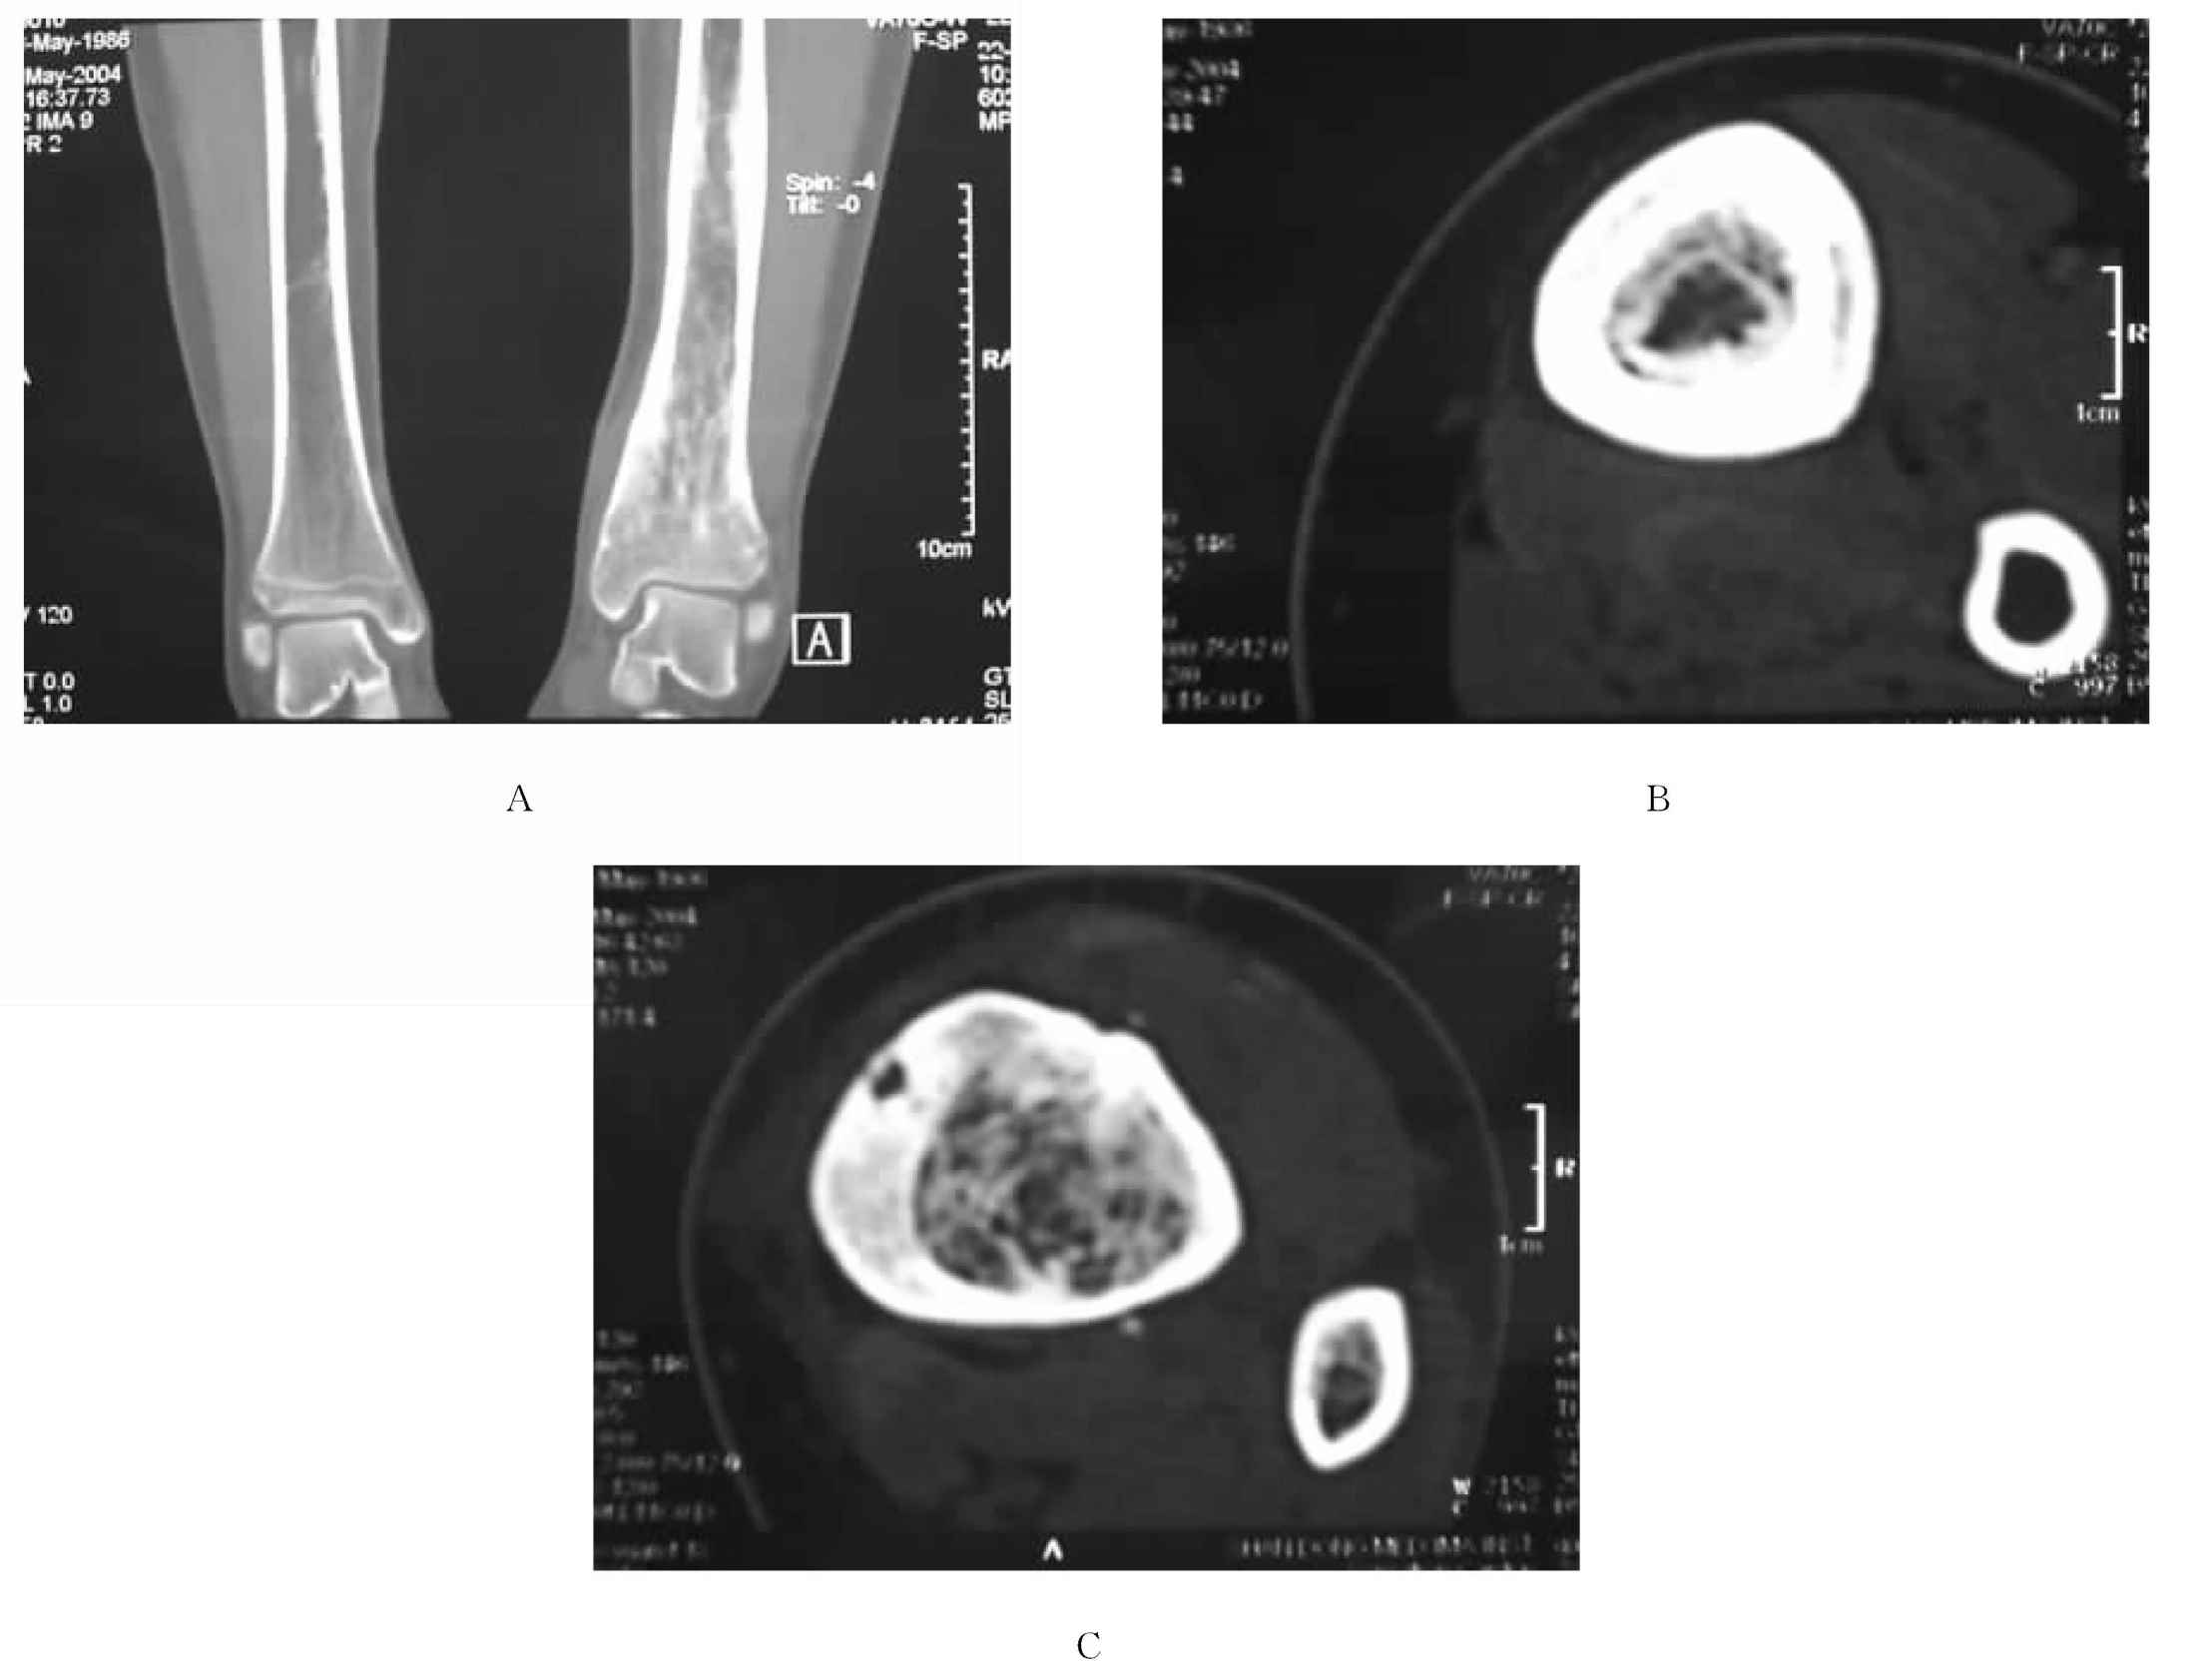
\includegraphics[width=.7\textwidth,height=\textheight,keepaspectratio]{./images/Image00426.jpg}
 \captionsetup{justification=centering}
 \caption{左侧胫骨慢性化脓性骨髓炎\\{\small 左侧胫骨中下段皮质增厚、髓腔密度增高、骨内膜增生}}
 \label{fig22-10}
  \end{figure} 

总之,其基本的征象有软组织肿胀、骨质破坏、骨质疏松、骨质增生硬化、骨膜反应及骨包壳6种。但以经久不愈的瘘管、大块状死骨以及死腔为其特征。

3.慢性硬化性骨髓炎:好发育长骨骨干如胫骨、腓骨、尺骨和跖骨等处。呈病变范围较大的骨密度增高区,骨皮质增厚,骨髓腔狭窄或消失。一般无骨质破坏,如有较平片易发现(图\ref{fig22-11})。相邻脂肪间隙内可有斑片状略高密度灶。

\begin{figure}[!htbp]
 \centering
 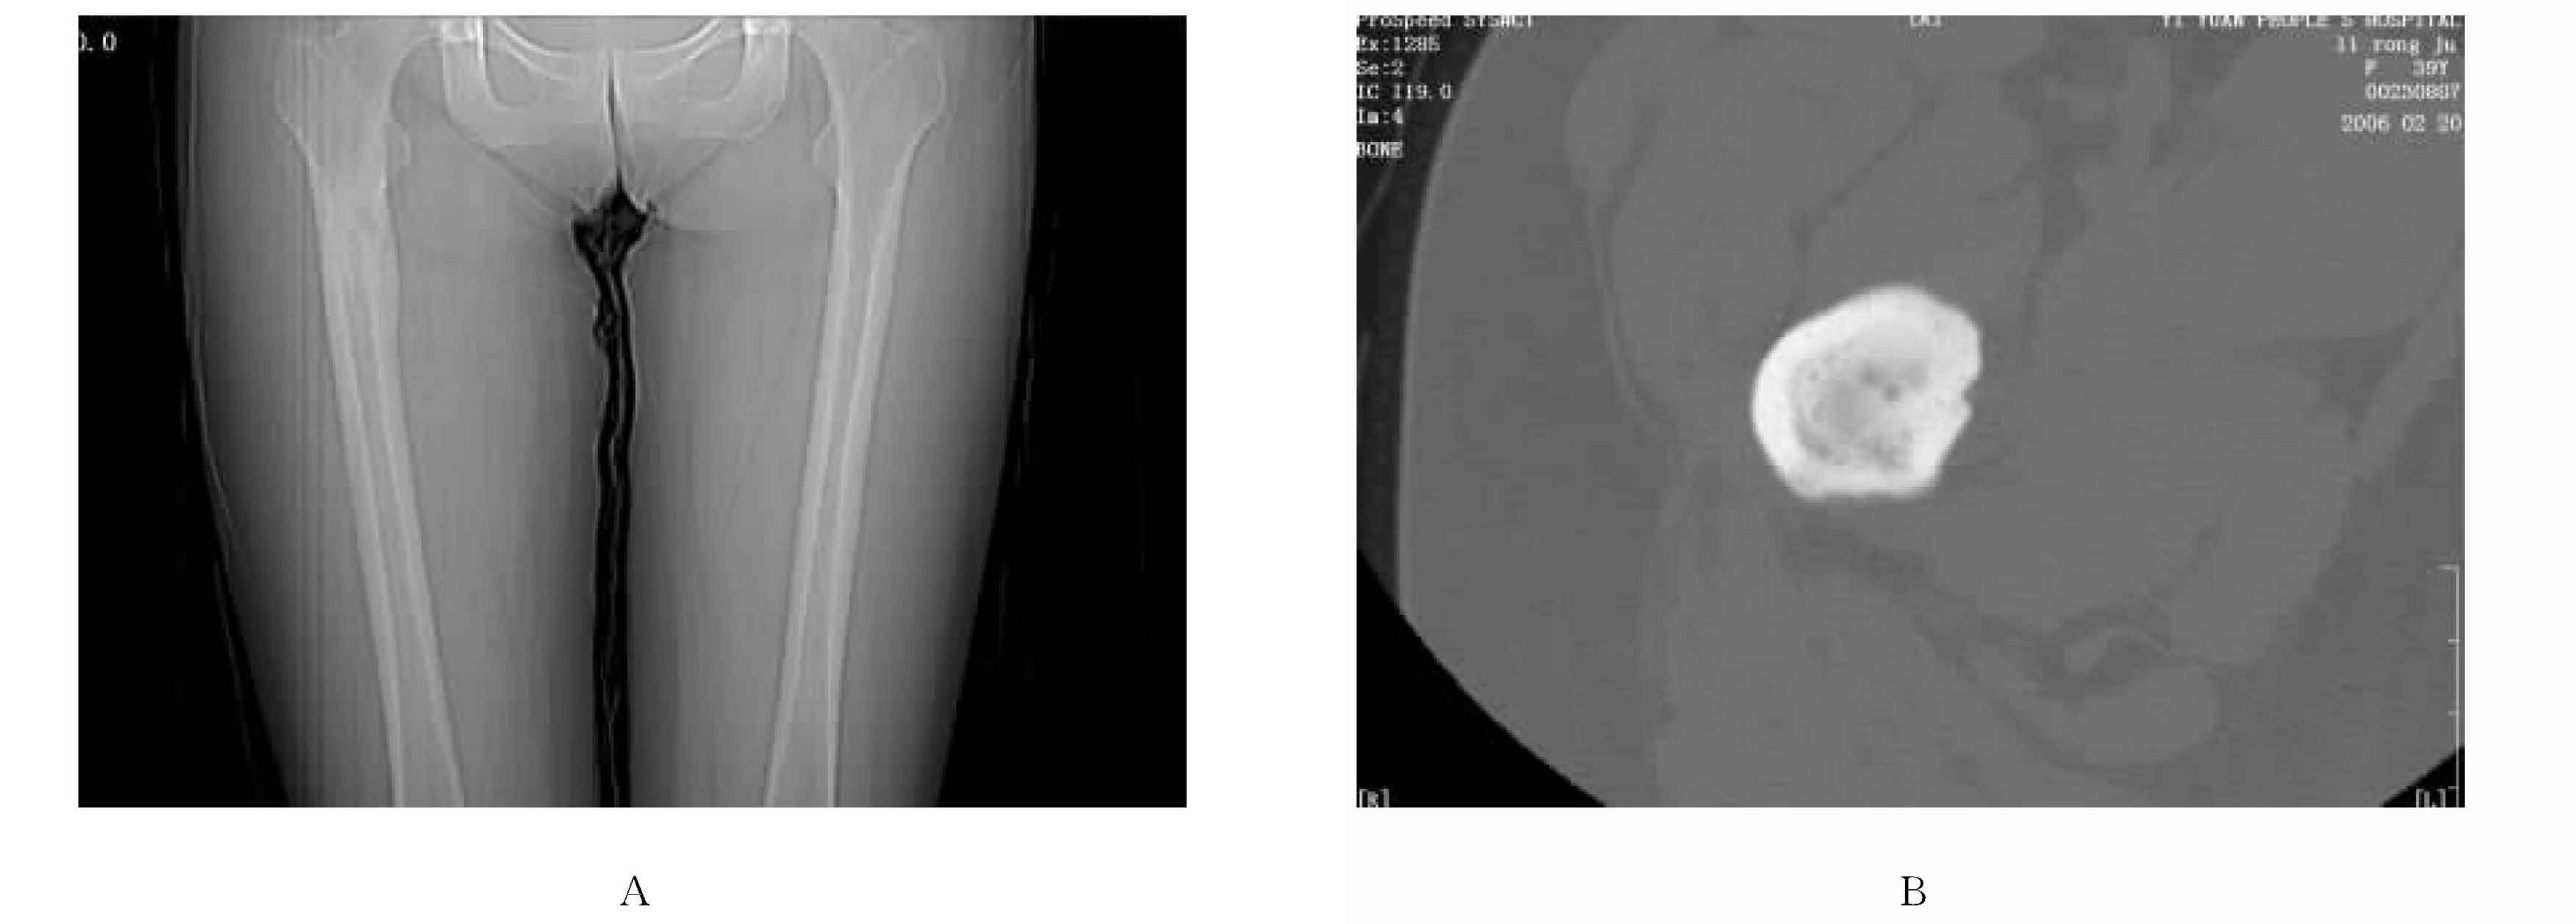
\includegraphics[width=.7\textwidth,height=\textheight,keepaspectratio]{./images/Image00427.jpg}
 \captionsetup{justification=centering}
 \caption{右侧股骨近端硬化性骨髓炎\\{\small 局部骨皮质增厚,骨髓腔基本消失}}
 \label{fig22-11}
  \end{figure} 

4.慢性局限性骨脓肿:常发生于胫腓骨上端、股骨下端、肱骨下端的干骺区。于长骨干骺端的中央有圆形或椭圆形密度较低的骨质破坏区,边缘较整齐;周围有高密度硬化圈,硬化带与周围正常骨质界限不清(图\ref{fig22-12})。少数不典型,有两个或多个分叶状的破坏区。破坏区一般无死骨,偶有很小的死骨。局部软组织无肿胀,亦无瘘管形成,很少有骨膜增生。

\begin{figure}[!htbp]
 \centering
 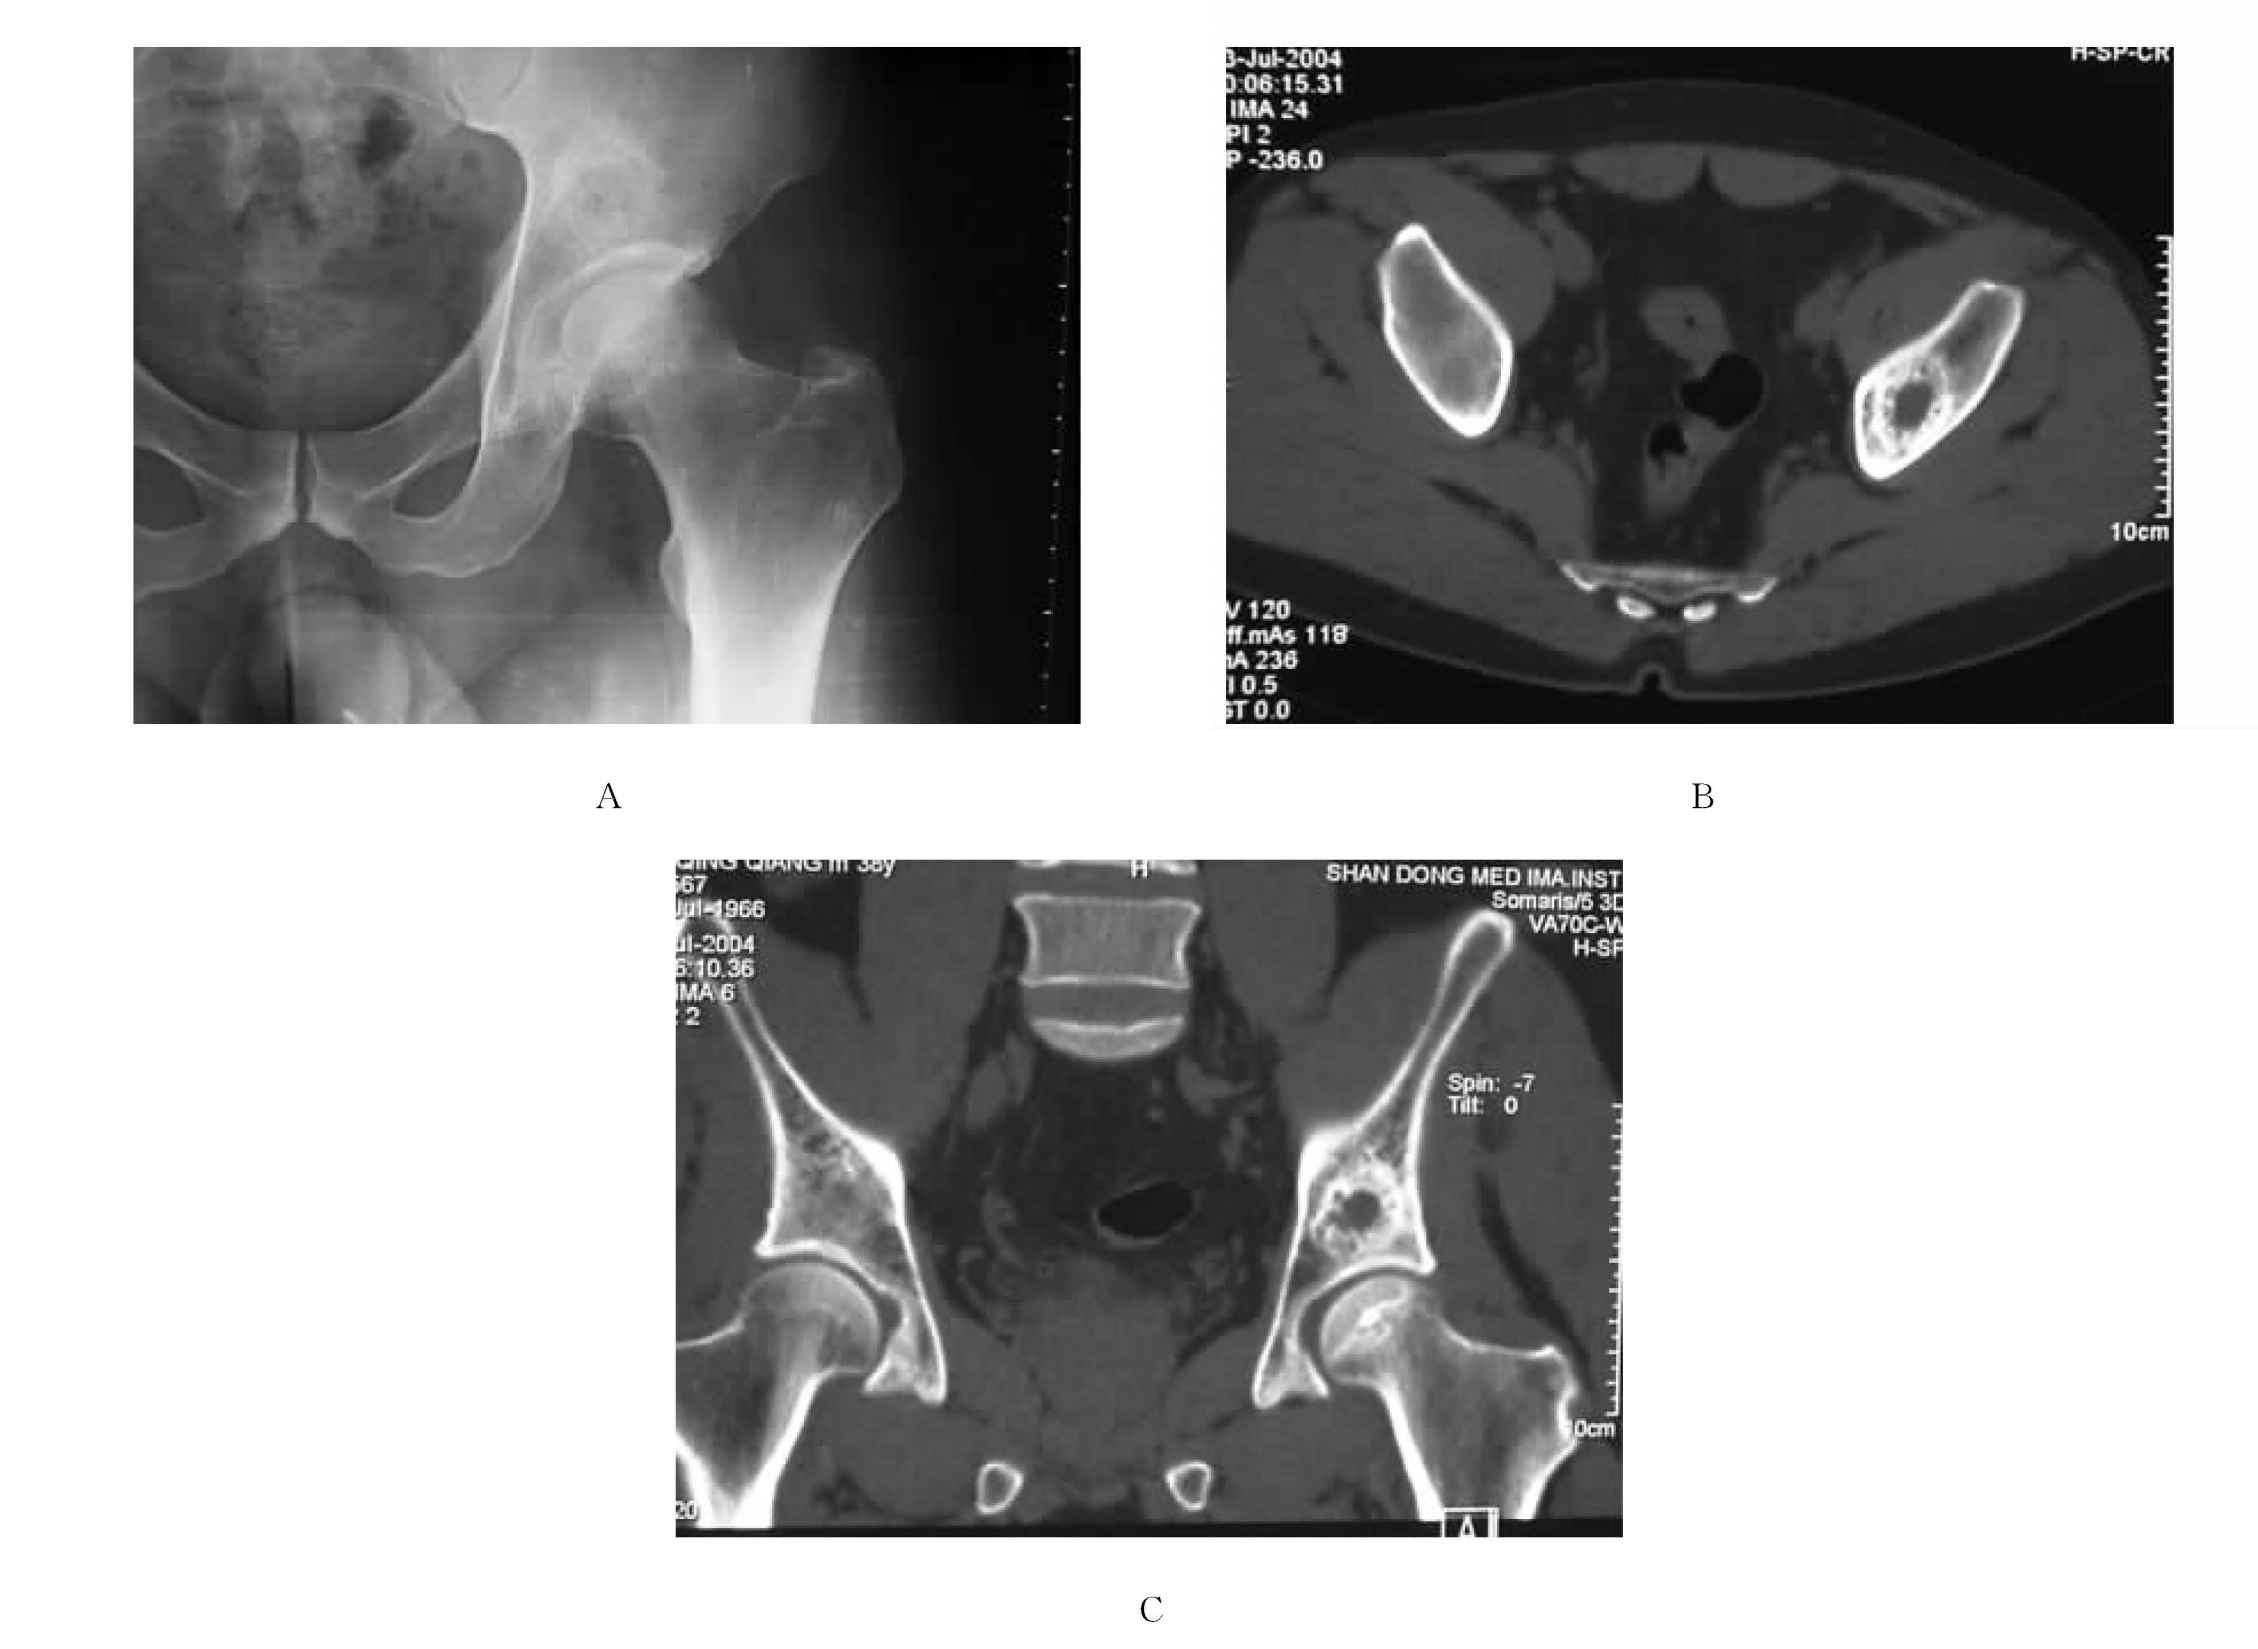
\includegraphics[width=.7\textwidth,height=\textheight,keepaspectratio]{./images/Image00428.jpg}
 \captionsetup{justification=centering}
 \caption{左侧髂骨体部慢性局限性骨脓肿\\{\small 左侧髂骨体部有圆形骨质破坏区,边缘较整齐,周围有高密度硬化圈}}
 \label{fig22-12}
  \end{figure} 

5.软组织异常对化脓性骨髓炎的诊断和鉴别诊断价值:①软组织肿胀通常骨髓炎较恶性肿瘤更为广泛;②软组织内脓肿样囊腔为骨髓炎的特异性征象;③软组织肿块多见于恶性骨肿瘤,是其最常见的征象之一;④软组织肿块边缘残留骨壳或壳样钙化见于恶性骨肿瘤;而骨膜下脓肿表面的骨膜化骨多围绕脓肿整个表面、粗细均匀,包绕低密度的脓液或液气;⑤软组织肿块内的肿瘤骨或瘤软骨钙化,分别为成骨肉瘤和软骨类恶性肿瘤的较特异征象;⑥软组织内气体、脂液平面和窦道均为骨髓炎的可靠征象。

\subsection{化脓性关节炎}

本病系化脓性细菌感染滑膜而引起的关节内感染。可发生于任何年龄,但以儿童和婴儿多见。

\textbf{【病因病理】}
致病菌主要有葡萄球菌、溶血性链球菌、肺炎链球菌、脑膜炎球菌、淋病球菌等。感染途径有血行感染、邻近软组织感染或骨髓炎直接蔓延、外伤或穿刺直接感染。

致病菌首先引起滑膜充血、水肿、白细胞浸润和关节内浆液性渗出。随后,滑膜坏死,关节腔内为脓液。白细胞分解释放出大量蛋白酶,它能溶解软骨和软骨下骨质。愈合期关节腔内形成肉芽组织,最后发生纤维化或骨化,使关节发生纤维性强直或骨性强直。

\textbf{【临床表现】}
发病急骤,常有寒颤、高热;受累关节剧痛,并有红、肿、热及功能障碍。实验室检查白细胞和中性粒细胞计数升高,ESR增快。

\textbf{【CT表现】}
最常受累的部位是膝、髋关节,其次为肘、肩和踝关节,骶髂关节亦可受累。

早期显示关节周围软组织肿胀,密度稍减低,界限不清,关节腔内可见多少不等的低密度积液,CT值20~40Hu。产气菌感染时,关节腔内或软组织内可有气体。增强扫描关节滑膜可呈线样强化,软组织强化不显著。

当关节软骨破坏后,关节间隙变窄,继而出现骨性关节面及相邻骨质侵蚀破坏和其周围不规则硬化,以关节持重区为著。感染严重时,可出现邻骨骨髓炎和关节病理性脱位。关节积液密度升高,CT值可达50~60Hu,甚至与关节囊和周围组织分辨不清,但增强扫描有利于显示无强化的脓液。脓液也可穿破关节囊在软组织内形成脓肿,增强扫描脓肿壁明显强化。

在小儿可显示中等偏高密度的关节软骨残缺不全,密度减低,边缘模糊毛糙。软骨下骨质有多囊状破坏,周围可有硬化,以持重部为著。周围骨质疏松。增强扫描可见关节囊内层强化明显、厚薄不均,部分可累及关节周围滑囊。

\subsection{骨关节结核(概述)}

骨与关节结核95%以上继发于肺结核。由血行播散的结核菌最易侵犯血供丰富的骨松质如椎体、干骺端、骨骺等,偶尔可累及长、短管状骨骨干以及扁骨。据王云钊统计,脊柱结核达50.9%;关节结核发生率依次为髋15.8%,膝12%,肘9%,踝4.7%,足3.9%,肩1.7%,手1.0%;骨干1.0%。但也有统计髋关节和膝关节约占80%,其次为骶髂关节和肘、肩、踝等。

\textbf{【病理】}
骨关节结核病理所见有渗出、变质、增殖3种基本病变。①渗出以淋巴细胞和单核细胞浸润为主;②变质性病变主要是干酪坏死;③增殖性病变主要是上皮样细胞的增殖及散在的郎罕巨细胞,中心常有干酪坏死。渗出和增殖性病变均可发生干酪样坏死。

成人骨结核较少发生骨膜反应,但在结核灶侵犯骨皮质表面时,可出现较局限的骨膜反应。儿童期骨结核均可出现骨膜反应。

\textbf{【临床表现】}
病程缓慢,各种病症均较轻,可有低热、血沉增速等。早期局部可有疼痛、肿胀和功能障碍等,无明显发红、发热。后期可有冷脓肿产生,穿破后形成窦道,可继发化脓性感染。长期病变可导致畸形和严重的功能障碍。

\textbf{【影像学征象】}
骨关节结核的基本影像学征象:①局部软组织肿胀;②患肢废用性骨质疏松、骨质破坏;③骨质增生硬化、骨膜反应;④死骨及干酪钙化等。

\subsection{骨骺与干骺端结核}

病灶多为局限性,好发于股骨上端、尺骨近端和桡骨远端,其次为胫骨上端、腓骨远端和股骨下端。病变可向关节方向发展为关节结核。本型结核较少穿破皮肤形成窦道。

\textbf{【CT表现】}
可分为中央型和边缘型,其中骨骺结核多为中央型,病灶多为单发。

1.中央型:表现为边缘较清楚的圆形或椭圆形骨质破坏区,也可多个融合成分叶状。周围有少量不规则骨质硬化,其内可有沙砾状死骨。病灶侵及皮质时可有轻微层状骨膜增生。病变常跨越骺板同时侵犯骨骺和干骺,而且病灶多向关节方向穿破、很少向骨干方向蔓延(这与化脓性感染相反),是结核的特点。

2.边缘型:多见于骺板融合后的干骺端,特别是长管骨的骨突处。早期局部骨皮质侵蚀糜烂,之后出现骨质边缘溶冰状的单纯溶骨性缺损,可伴薄层硬化。一般无死骨。

\subsection{长骨骨干结核}

其发病率最低,多见于儿童和青少年,30岁以上极少见。好发于无或少有肌肉附着的骨骼,如前臂和小腿骨等。为局限性慢性感染,渐渐的将骨松质吸收破坏,继而侵犯骨皮质,并可引起骨膜反应。

\textbf{【CT表现】}
通常为单发,病灶大多偏于骨干一侧,离干骺端有一定距离。病灶呈单个或多个、较小的圆形或椭圆形骨质破坏,边缘清晰,周围硬化较显著。常有层状骨膜增生。髓腔与皮质界限不清,但病变范围较局限。这种表现类似于慢性硬化性骨髓炎。有时呈膨胀性改变,使骨干呈梭形扩张有一定鉴别意义。

\subsection{扁骨结核}

扁骨结核分局限型和弥漫型,以前者多见。

\textbf{【CT表现】}
①局限型:呈囊样骨质破坏,时间久、病灶稳定者可有硬化边缘,病变多单发,亦可多发。②弥漫型:少见,表现为广泛的鼠咬状骨质破坏。

1.颅骨结核:好发于额、顶骨,其次为枕、颞骨,颅底骨少见,分为局限型和弥漫型。①局限型:表现为圆形或卵圆形骨质破坏,1~4cm不等。病灶边缘清晰锐利,有时可有硬化边,其内可见“纽扣样”死骨,邻近软组织肿胀。严重者颅内可有低密度灶,增强扫描脑膜可强化。②弥漫型:骨质破坏呈匍匐状向四周浸润,范围广泛且不规则,界限不清,可形成软组织脓肿和窦道。

本病的颅骨破坏不受颅缝限制;而骨髓炎骨质硬化大于破坏,死骨形成机会多,结合临床可予鉴别。嗜酸性肉芽肿破坏区呈地图样外观,边缘清楚,周围无明显骨质硬化,结合临床多可鉴别。

2.髂骨结核:必须不累及骶髂关节和髋关节才属该病的范畴。病灶常见于髂骨翼和髂骨嵴,多单发而局限。表现为界限不清的骨质破坏,边缘可稍有骨质增生硬化,其内可见死骨(但平片不易发现)。局部可见软组织肿块,增强扫描可见环状强化的脓肿。如软组织内有斑片状钙化则有助于结核的诊断。有时脓肿可达臀间肌、腹股沟、股上部等处。

化脓性病灶周围骨质增生硬化显著,常见明显死骨形成;且如病灶位于髂骨下部应多考虑为化脓性病灶。

3.胸骨结核:主要表现为骨质破坏,可呈较为局限的囊状或不规则破坏区,也可表现为较广泛而散在的不规则破坏或虫蚀样破坏。局部软组织肿胀。

4.肋骨结核:①局限型:局限于肋骨后侧,多表现为肋骨下缘局限的缺损,边缘规则,可有骨膜增生。②弥漫型:病变较广泛地累及肋骨的髓腔引起结核性骨髓炎。表现为多个不规则的骨质破坏区,可有骨膜增生,但呈囊状并使病骨膨大者较少见。

此外,无论是局限型还是弥漫型,破坏区总残留一些骨质或死骨存在,可伴有广泛胸膜增厚,还可见局部胸壁软组织肿胀,甚至形成脓肿。应注意与胸壁内非原发于肋骨的结核相鉴别。

5.坐骨和耻骨结核:病灶多呈囊状破坏,病骨膨大显著。破坏区边缘稍有硬化,可伴死骨,邻近可有骨膜反应。耻骨联合的结核多从一侧开始,但都会累及对侧,多有碎屑状死骨(图\ref{fig22-13})。邻近软组织可有肿胀、脓肿形成及斑片状钙化。

\begin{figure}[!htbp]
 \centering
 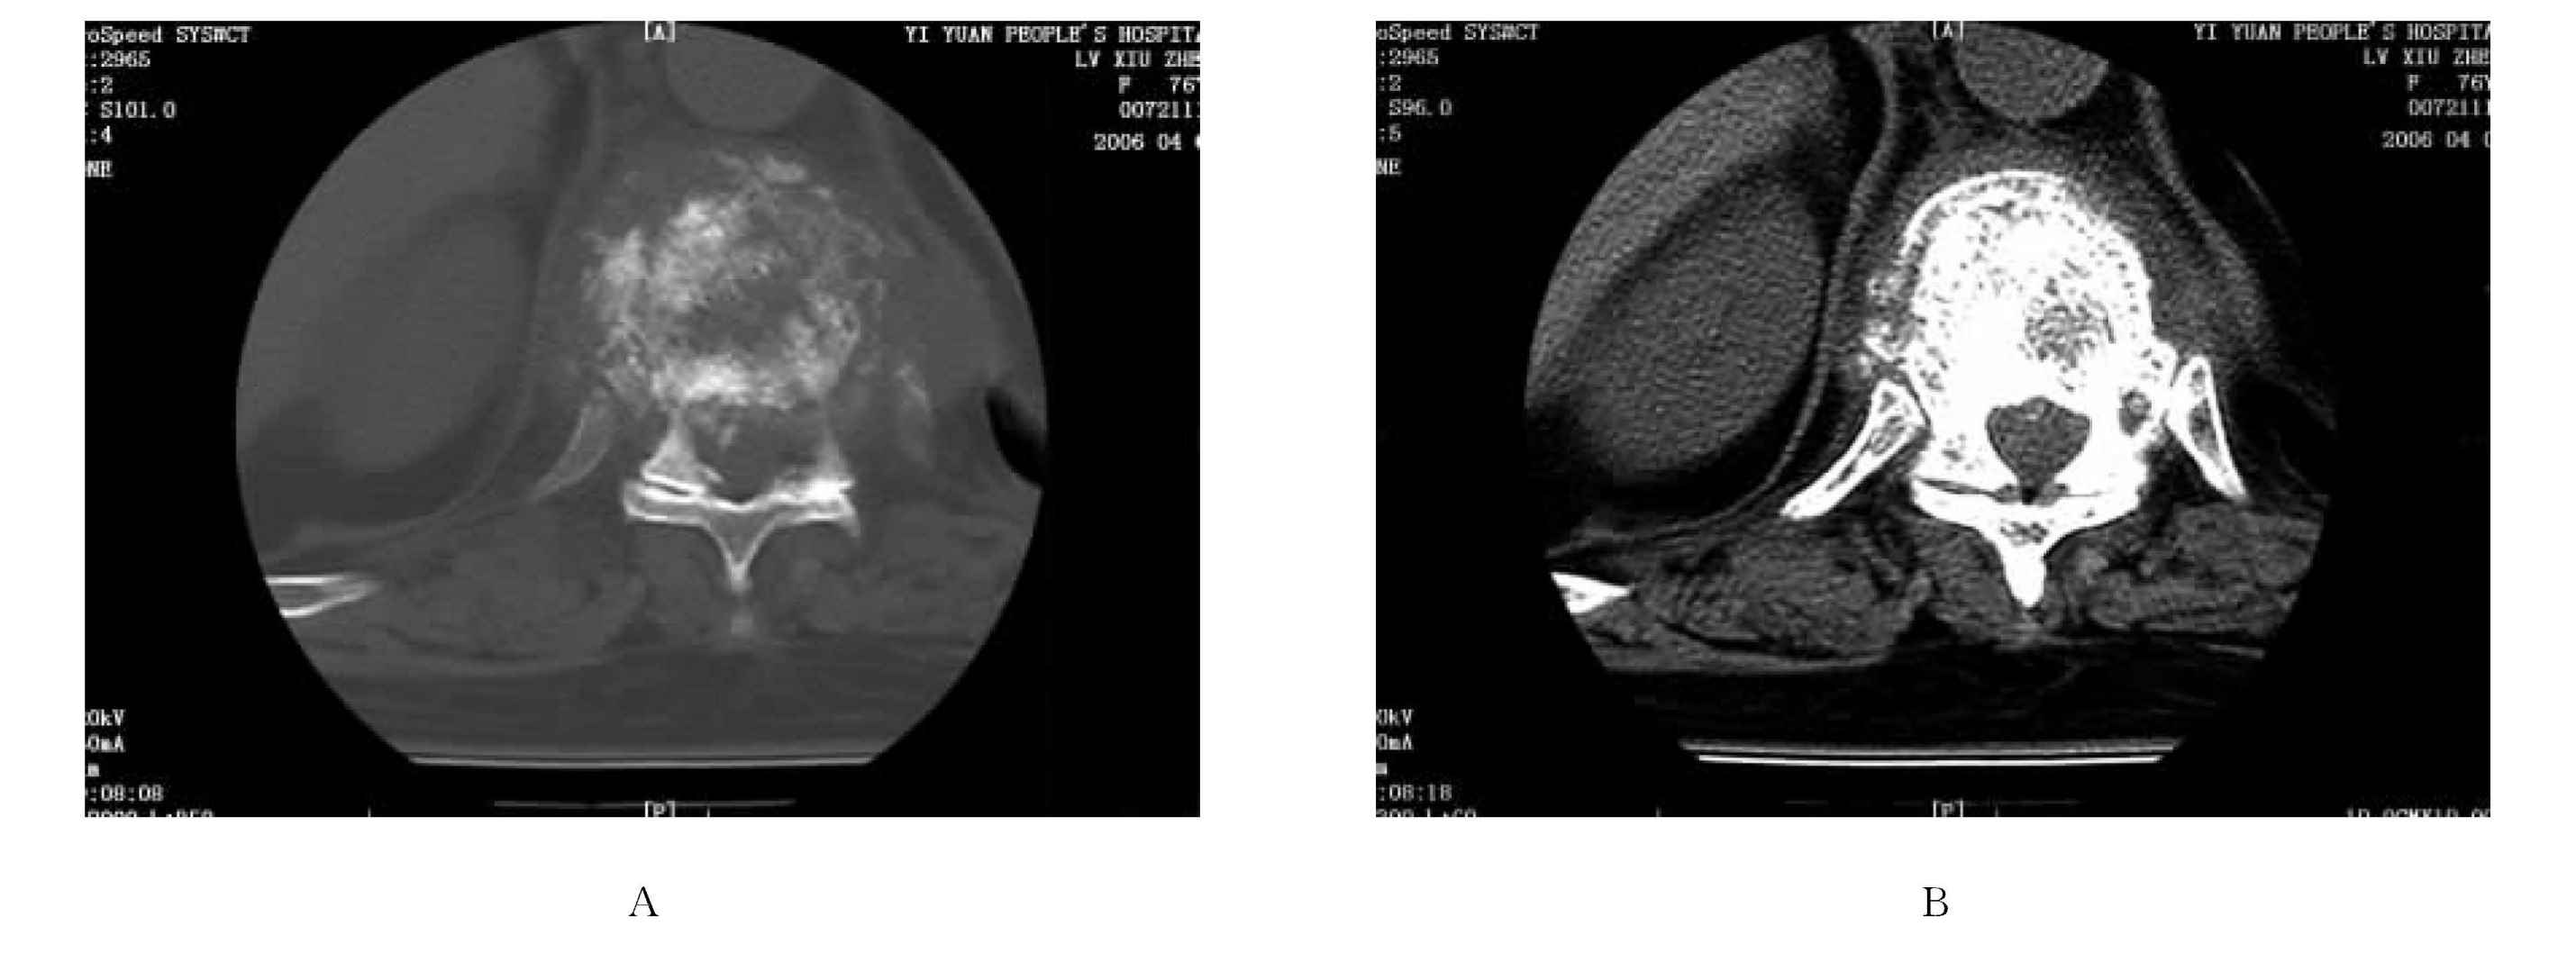
\includegraphics[width=.7\textwidth,height=\textheight,keepaspectratio]{./images/Image00429.jpg}
 \captionsetup{justification=centering}
 \caption{耻骨联合结核\\{\small A、B为同一患者。A.左右侧耻骨联合均有不规则囊状骨质破坏区,边缘稍有硬化,局部有碎屑状死骨;B.邻近的左侧深部软组织内有脓肿,其内也有斑点状钙化}}
 \label{fig22-13}
  \end{figure} 

\subsection{脊柱结核}

\textbf{【病理】}
可分为两大类:①椎体结核:又分为中心型、边缘型和韧带下型。②附件结核:发生于椎弓和骨突的结核。

椎体结核的中心型多见于10岁以下儿童,以胸椎多见;边缘型多见于成人,以腰椎多见。儿童供应椎体的主要血管为后脊椎动脉的一个分支,从后壁进入椎体的中央部分,此时椎体周围尚有一层较厚的软骨,因此病灶一般在椎体中央近前方开始。成年人时供应椎体的主要血管为肋间动脉和腰动脉,从前方进入,沿骨膜下分支,所以病灶多从椎体前缘、骨膜下以及前纵韧带下的椎间盘开始。

同时应认识到:①中心型因多见于儿童,椎体较软而松,而且皮质分化程度差,所以易向上下发展,可连续累及多个椎体和椎间盘。②边缘型病灶有较久的局限于一个椎体的趋势,亦可沿着骨膜下和前纵韧带向上、下进展而累及邻近椎体,但多只限于两个椎体,累及3个以上椎体者少见。椎体的破坏和塌陷一般不如中心型明显。还应认识到,脊柱结核亦可多个脊椎相间发病,即跳跃型病变。

\textbf{【临床表现】}
大多数病人发病隐匿,病程缓慢,症状较轻。有的病人已脊柱畸形,但仍能从事劳动。全身症状可有低热、乏力和食欲差。局部常有脊柱活动受限,颈、背或腰痛,多为酸痛或钝痛,少见剧痛。压迫脊髓、食管、气管可引起相应的症状。腰大肌脓肿可注入髂窝,甚至到达臀部。

\textbf{【CT表现】}

1.早期:可仅见椎前软组织肿胀,无明显骨质破坏和椎间盘受侵及其所致的椎间隙变窄。

2.进展期:①可见椎体或附件融冰样、碎玻璃样明显骨质破坏,邻近椎间隙变窄(图\ref{fig22-14})。②均伴周围脓肿形成,冷脓肿张力高,边缘多清晰,其内可有钙化影;增强扫描脓肿壁呈环状强化,厚薄均匀。此外,腰椎冷脓肿可沿腰大肌至股骨小转子处,甚至引起髋关节结核(图\ref{fig22-15})。③椎间盘大多数密度不均、椎间隙变窄。④椎体后缘或附件的骨质破坏,软组织突入椎管、死骨块突入椎管均可致椎管狭窄。



\begin{figure}[!htbp]
 \centering
 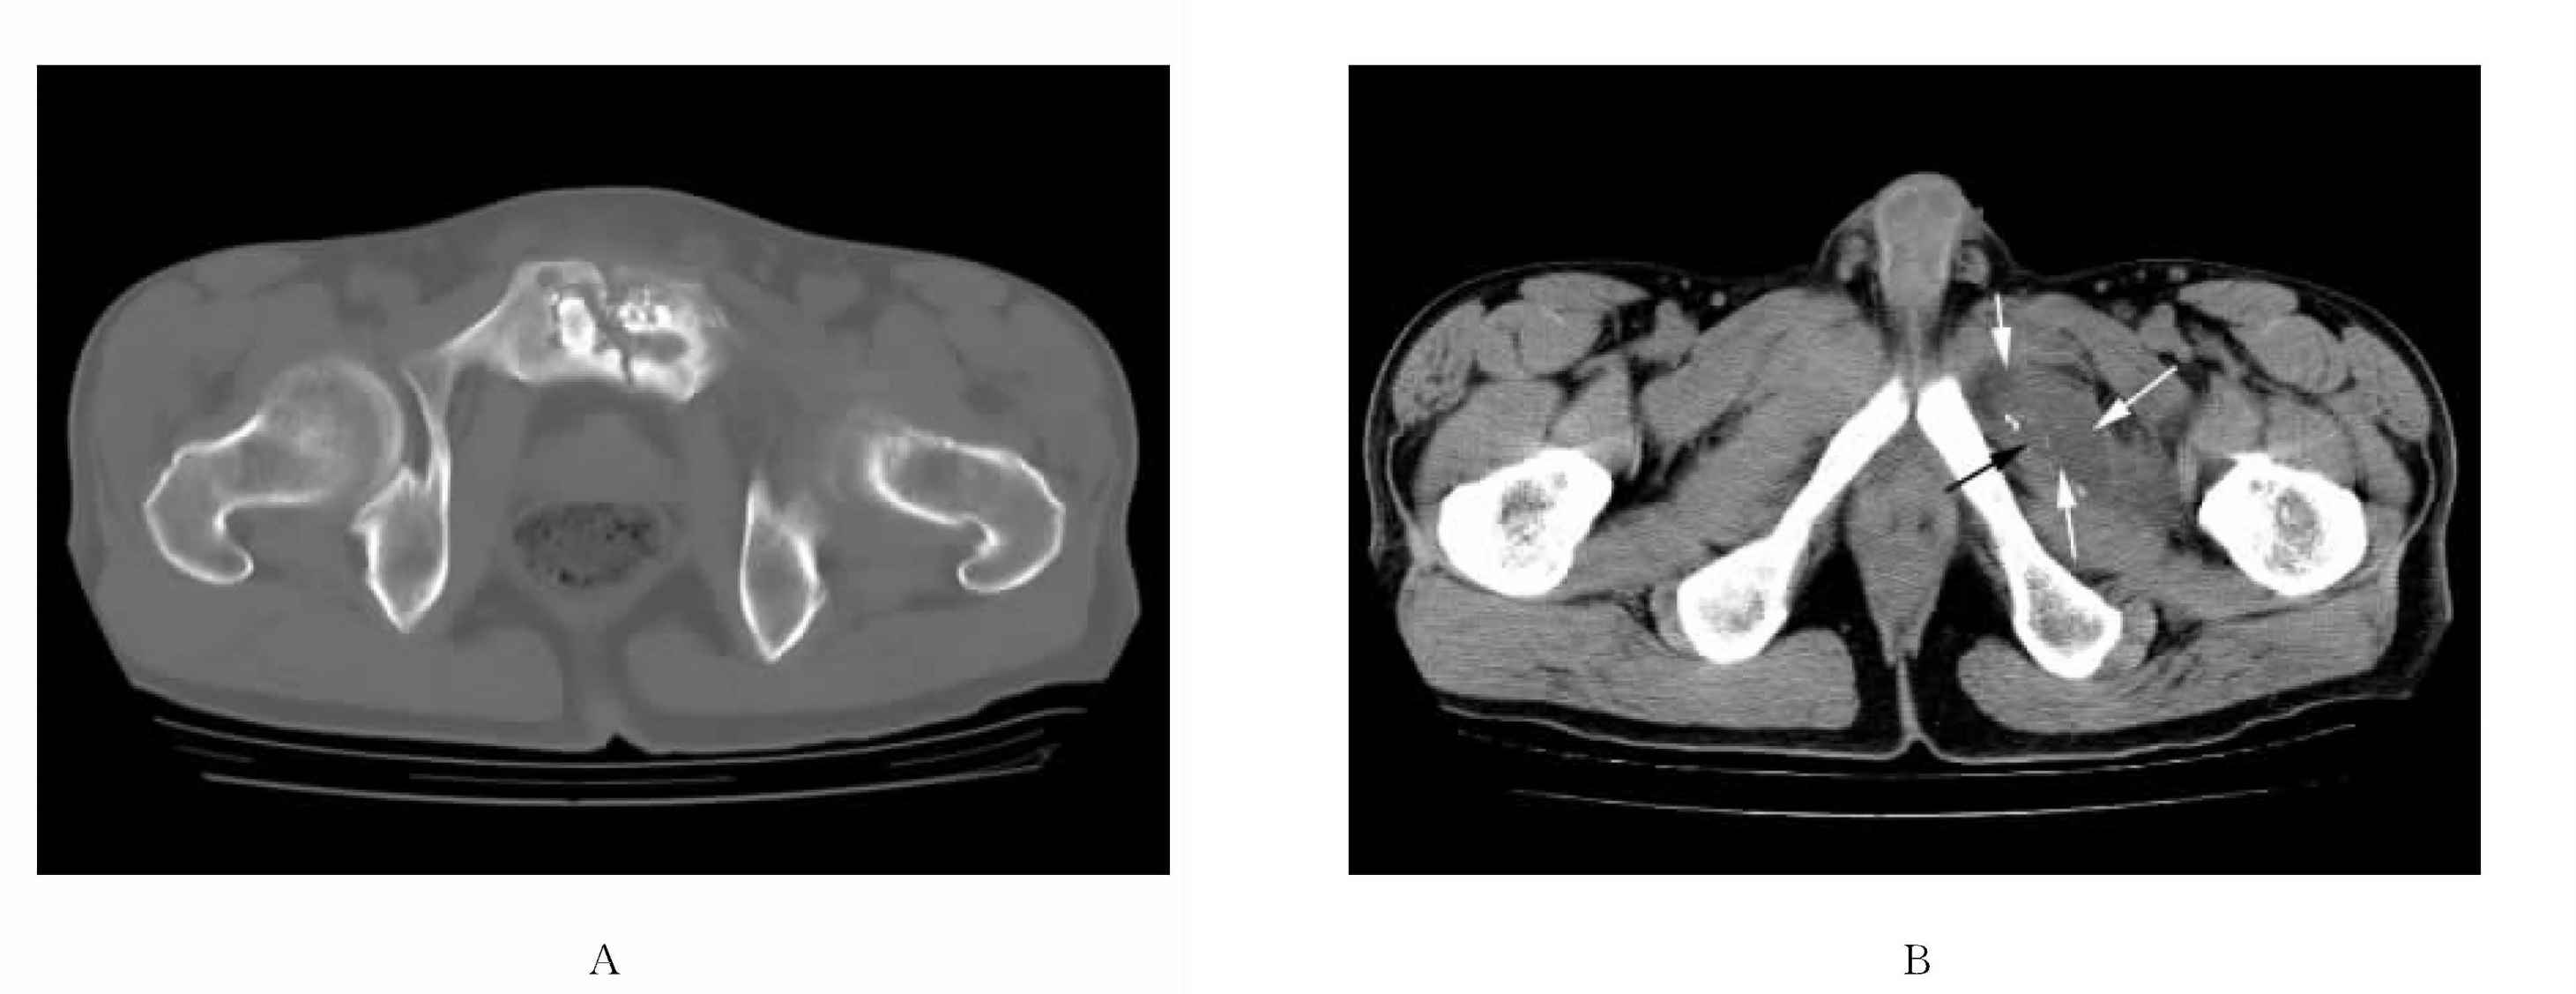
\includegraphics[width=.7\textwidth,height=\textheight,keepaspectratio]{./images/Image00430.jpg}
 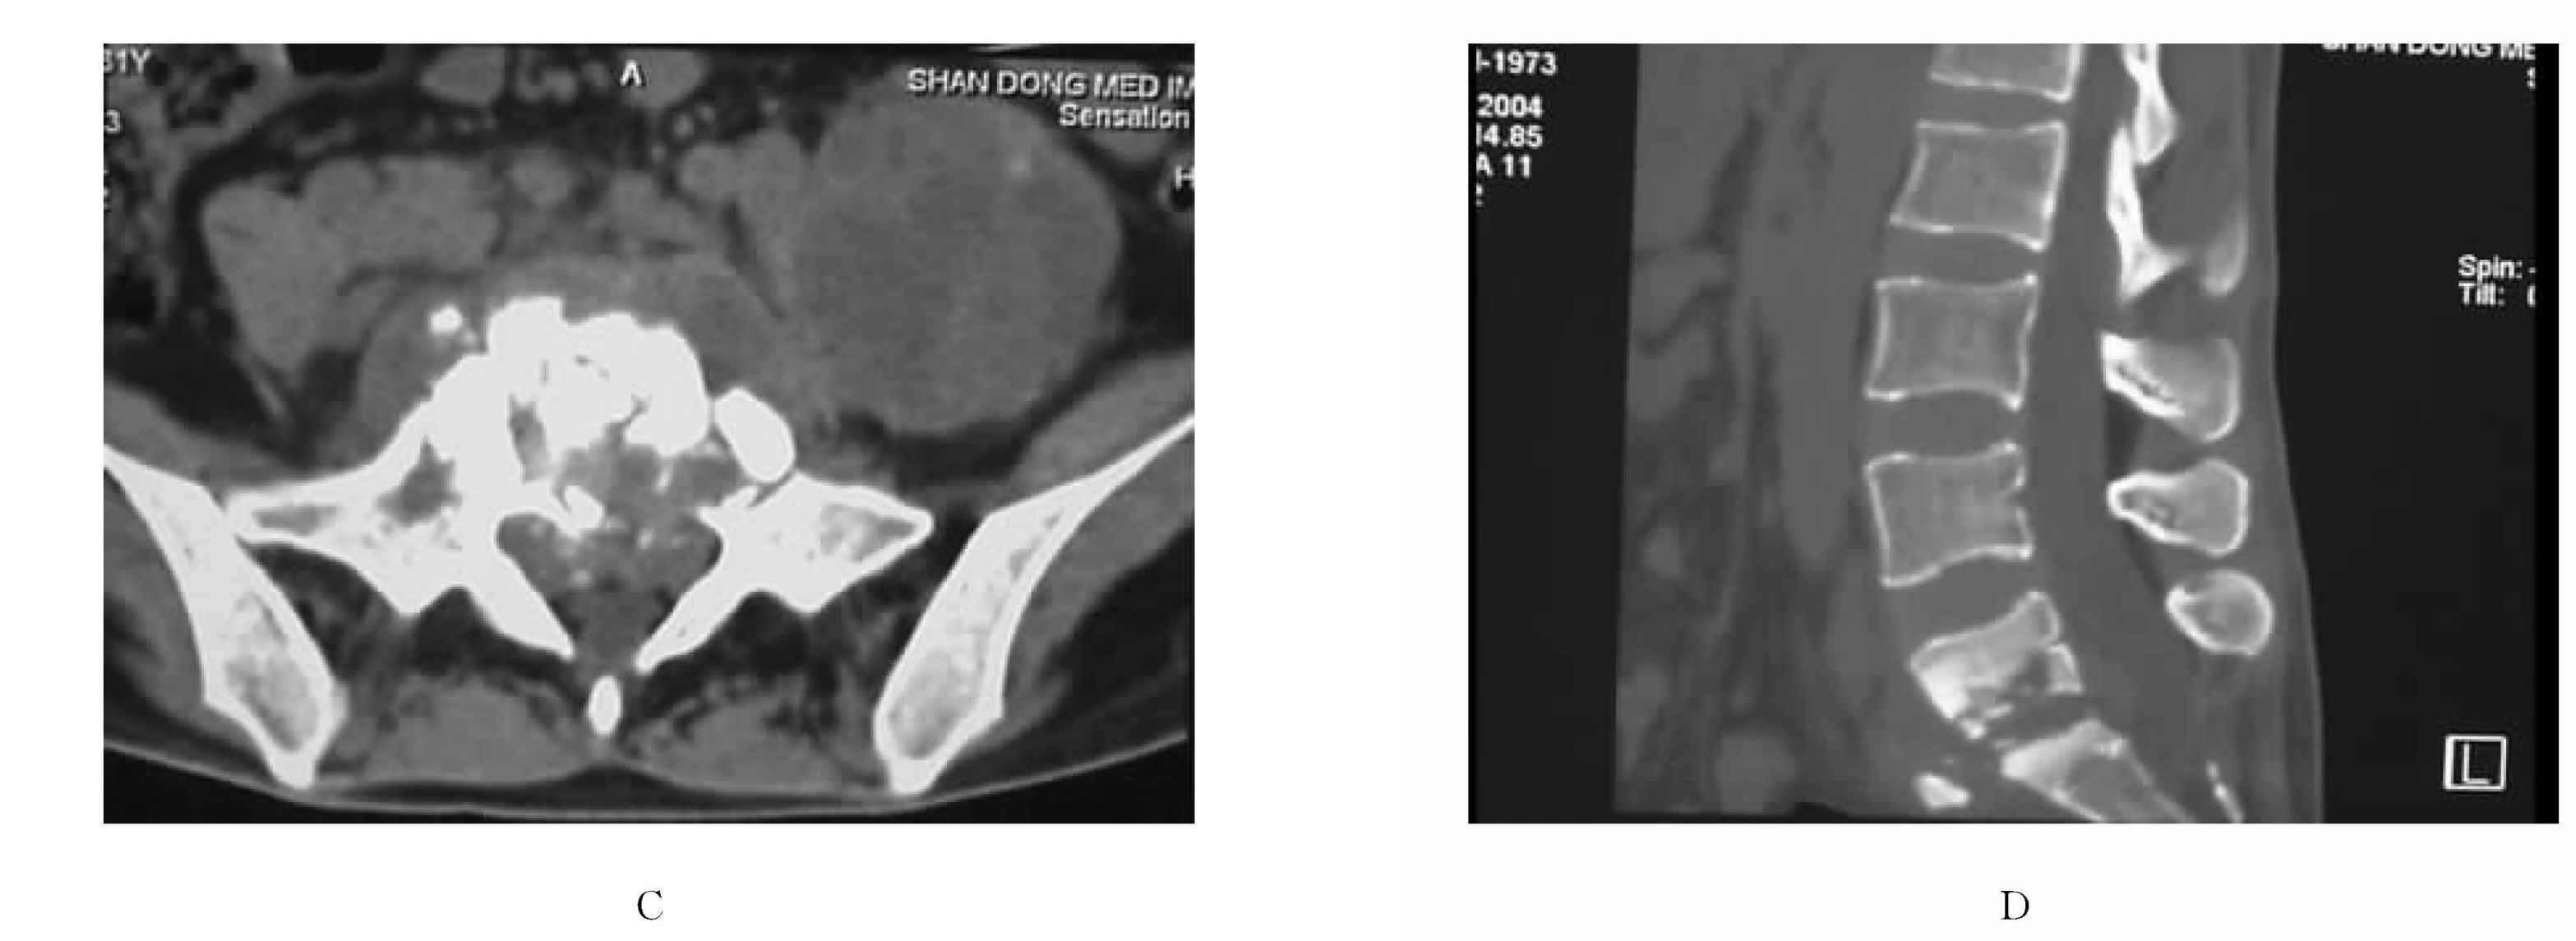
\includegraphics[width=.7\textwidth,height=\textheight,keepaspectratio]{./images/Image00431.jpg}
 \captionsetup{justification=centering}
 \caption{脊柱结核\\{\small A、B为同一患者,病灶位于胸椎;C、D为同一患者,病灶位于腰椎;均表现为碎玻璃样显著骨质破坏。C可见椎旁脓肿,以及左髂窝脓肿}}
 \label{fig22-14}
  \end{figure} 

\begin{figure}[!htbp]
 \centering
 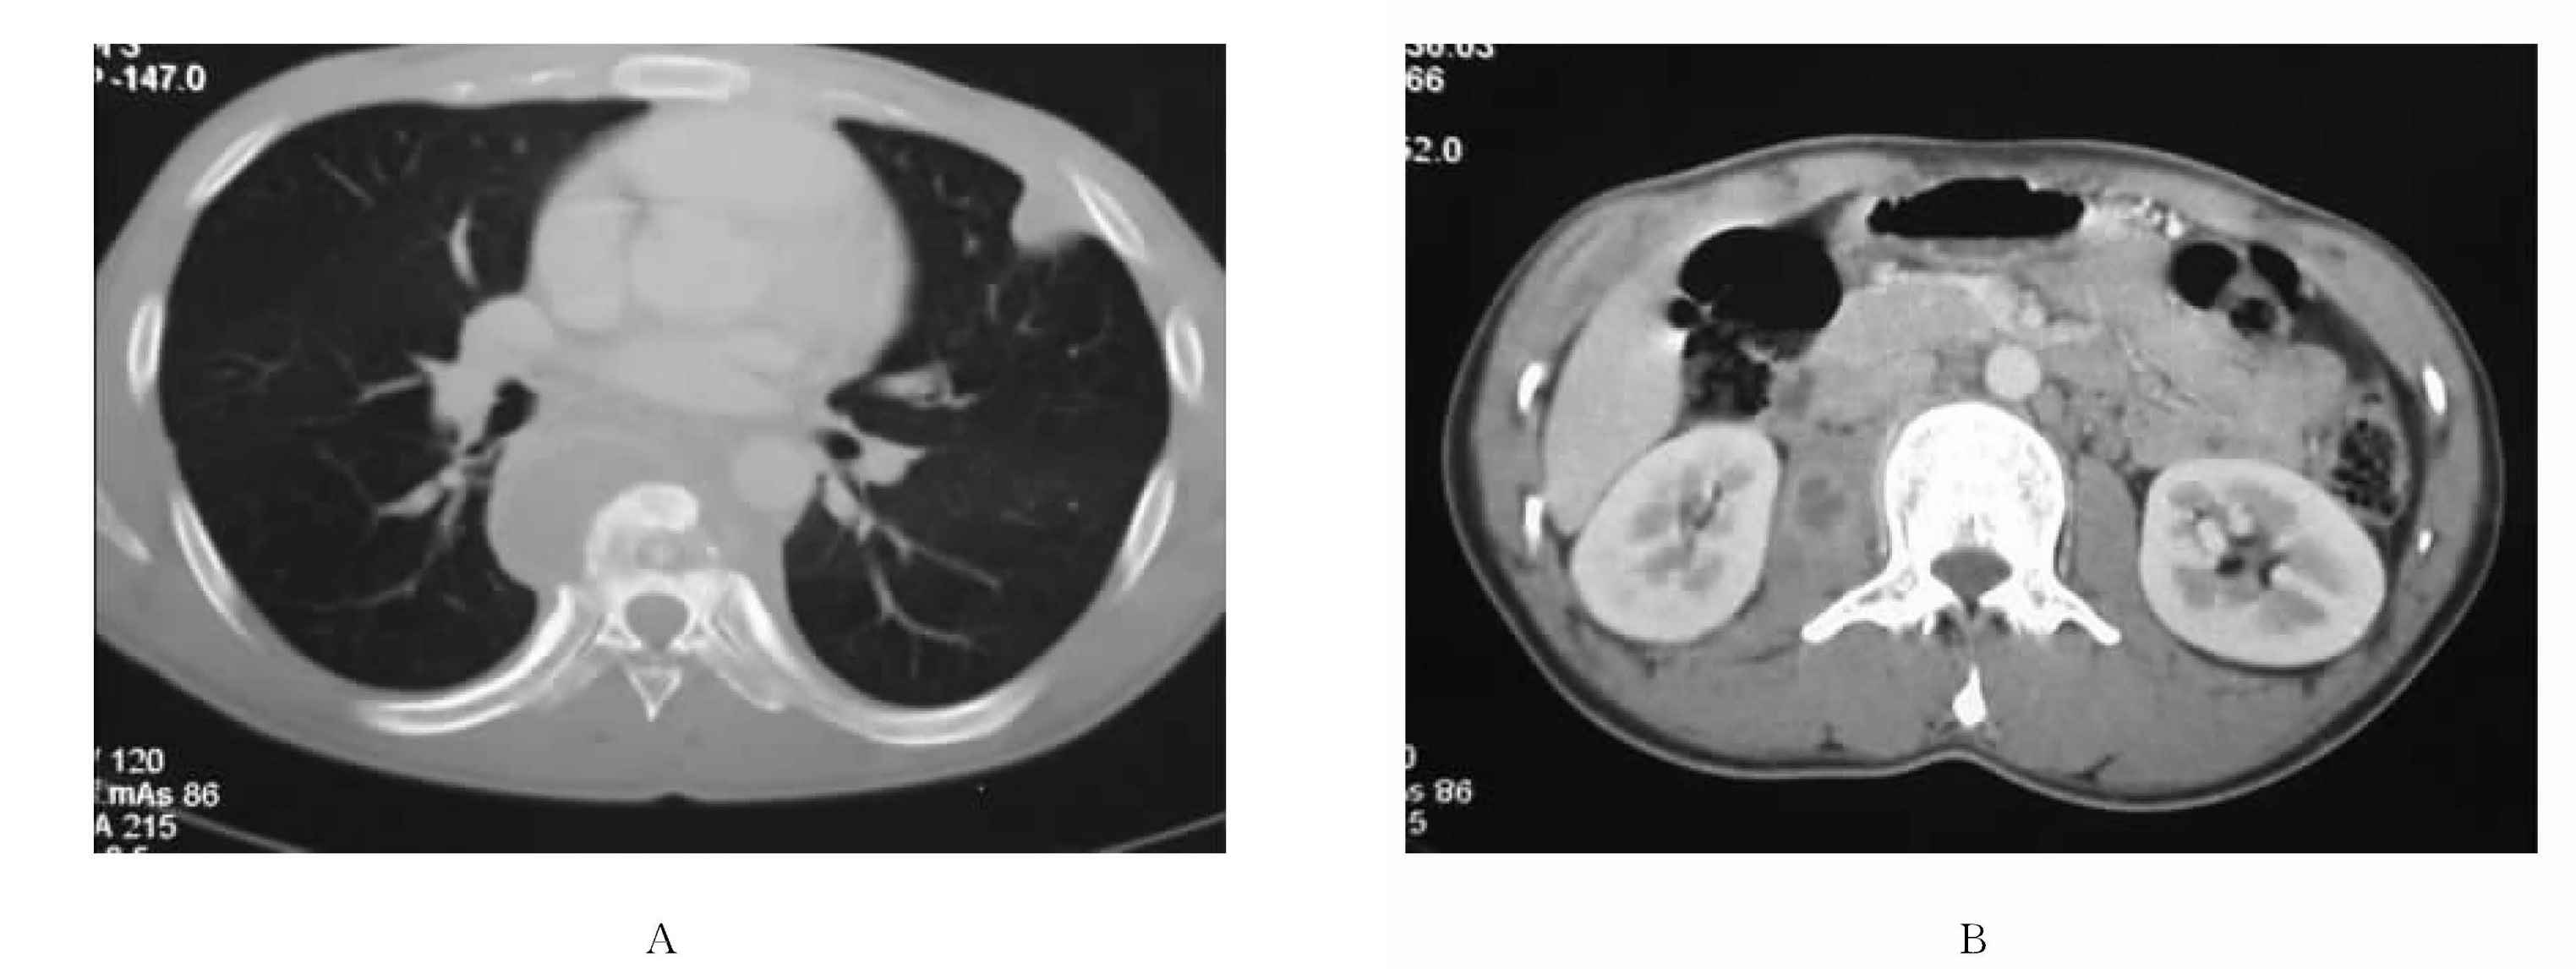
\includegraphics[width=.7\textwidth,height=\textheight,keepaspectratio]{./images/Image00432.jpg}
 \captionsetup{justification=centering}
 \caption{结核性椎旁脓肿\\{\small 胸椎结核冷脓肿位于右侧腰大肌内}}
 \label{fig22-15}
  \end{figure} 

3.愈合期:骨质破坏区边缘硬化,冷脓肿消失,弧形或不规则沙粒状钙化等仍存在。

4.并发症:①脊柱畸形:以后突最常见;②脊髓受累;③化脓性感染:表现为化脓性病变与结核病变共存。

总之,融冰样、碎玻璃样骨质破坏,破坏区内沙粒样死骨,冷脓肿形成是其典型表现。

\textbf{【鉴别诊断】}

1.化脓性脊柱炎:可分为椎间型、椎体型、骨膜下型和附件型。以胸腰椎多见,亦可多节段发生。①影像学表现与结核有许多相似之处,如椎体破坏、椎间隙狭窄、椎旁脓肿。但临床表现发病急,骨质破坏进展快,骨质增生出现早。早期诊断结合临床甚为重要,单纯影像学可难与结核鉴别。②结核继发化脓菌感染,亦可在骨破坏周围有增生表现,但其程度和范围均不及慢性化脓性脊椎炎那样广泛。此外,脊柱结核虽可有骨刺形成,但不至于形成慢性化脓性脊椎炎那样的骨桥。

2.椎间盘炎:多发生于儿童或手术后(包括介入治疗)并发症,致病菌主要为金黄色葡萄球菌。最常见的临床症状为腰背疼痛、肌肉痉挛,体温多为37.5~38℃,ESR增快。①影像学于术后2~4周即可见椎间隙变窄,椎间盘密度减低、边缘模糊且变扁变大,类似椎间盘膨隆;②随后可出现椎体骨质疏松、终板破坏及硬化表现,可有椎体融合表现(详见第二十三章第六节)。

3.布氏菌脊椎炎:常侵及多个椎体,骨破坏灶小(2~5mm)而多发,多局限于椎体边缘;病灶周围明显增生硬化,新生骨组织中又有新破坏灶形成;椎间盘破坏,关节面增生硬化,相邻骨密度增高;少或者无椎旁脓肿形成。

4.转移瘤:①结核以侵犯前半椎多见;而转移瘤未见仅破坏前半椎者,易累及椎弓根。②结核易侵及椎间盘而表现椎间隙狭窄,椎旁脓肿多呈对称性分布,范围较大,超出椎体上下的范围;而转移瘤及其他恶性肿瘤一般无椎间隙变窄,骨质破坏及椎旁软组织肿块均不对称,且软组织肿块范围局限。

但是应认识到:①胸、腰椎一侧性椎弓根破坏,除见于转移瘤外,亦可见于结核、先天性缺损。②并非恶性肿瘤一定无椎间隙变窄(即椎间盘受累所致)。

\subsection{关节结核}

本病占全身骨结核的30%~40%。多见于少年和儿童,男性稍多见,一般为单关节发病。好发于髋关节和膝关节,其次为骶髂关节和肘、肩、踝等。

\textbf{【病理】}
可分为两型:①滑膜型:是指结核杆菌经血源播散至滑膜形成的关节结核。②骨型:骨骺、干骺端结核直接蔓延并侵及关节滑膜和软骨者。但晚期关节和相邻骨质均有明显破坏时,则无法分型。

结核菌侵及滑膜,首先引起滑膜充血、水肿、渗出和增生,并逐渐形成特异性的肉芽组织。因关节渗出液中缺乏蛋白溶解酶,故出现关节软骨破坏较晚。随着病变进展滑膜肉芽组织首先破坏关节软骨,继而软骨下骨质。一般先破坏非持重部、接触面较小或非接触的关节边缘部分。但破坏一般比较缓慢,有时已完全剥离的软骨可长期存在,故关节间隙变窄出现较晚且不对称。

\textbf{【临床表现】}
多数发病缓慢。早期症状轻微,表现为关节酸痛和轻度肿胀,劳累后加重。活动期可有全身症状如发热、盗汗、食欲差、消瘦;关节肿痛、皮温不高、活动受限;血沉加快、结核菌素试验强阳性。病程长者,可伴有关节邻近肌肉萎缩。

\textbf{【CT表现】}
早期可见关节腔内和滑囊积液,呈水样密度。周围软组织肿胀,密度减低,脂肪间隙模糊、密度增高。增强扫描可见关节囊内层和滑囊壁轻到中度线样强化。

随病情进展可见关节囊膨大,内有大量略低于肌肉的肉芽组织,与周围软组织界限不清。关节腔内仍有水样密度的积液表现,与肉芽组织混杂存在。在小儿,骺软骨模糊、密度减低,严重者呈碎裂状表现。关节边缘可见不规则骨质破坏,边缘硬化,其内常有细小沙粒状死骨。骨型关节结核可清楚显示骨骺、干骺端的骨质破坏区及其内的细小死骨。增强扫描关节腔、滑囊内及破坏区肉芽组织呈显著不均匀强化,如破坏区内为干酪组织则无强化。脓液穿破关节囊在关节周围可形成脓肿,呈单囊或多囊状低密度灶,个别呈蜂窝状,增强扫描囊壁有明显强化。还可显示邻近的骨萎缩变细和骨质疏松、关节脱位和畸形等。痊愈期可见邻近骨端硬化、界限不清,还可见关节囊及周围软组织中有斑片状不规则钙化。

部分关节结核的特点分述如下:

1.肩关节结核:大多自肱骨头部开始,从滑膜开始者很少见,从肩峰开始者亦少见。肱骨头的病灶以肉芽组织增生为主,很少渗液,无脓肿形成,所以称为“干性骨疡”。

2.髋关节结核:发病率仅次于脊柱结核,在四肢关节结核中最多见。病变起自股骨头、颈部,亦可从髋臼上方开始侵入关节,从滑膜开始者较少见。

3.肘关节结核:早期骨质破坏多见于尺骨冠突和鹰嘴突,其次为肱骨外髁和内髁,桡骨小头较少累及。

4.腕关节结核:单纯滑膜型少见,以同时累及骨和滑膜多见。单纯滑膜型可仅表现为软组织肿胀和骨质疏松;骨型关节结核可见到某一腕骨或桡骨下端的骨质破坏。

5.膝关节结核:发病率仅次于髋部。膝关节为滑膜最丰富的部位,故病变多从滑膜开始,占80%;起源于股骨、胫骨、髌骨者占20%。

6.踝关节结核:滑膜型较骨型稍多见。骨结核多见于胫骨下端,外踝次之,内踝和距骨最少。

7.骶髂关节结核:多见于成人,多为单侧发病,常位于中下部。滑膜型早期可无明显异常,进而关节面糜烂、关节间隙增宽,随后有骨质破坏;骨型可见邻近原发病灶处的明显骨质破坏和小死骨。关节可有病理性脱位,邻近可有脓肿及窦道。病变附近骨质疏松不如其他关节结核,可见骨质硬化,晚期可有纤维性或骨性强直。

\textbf{【鉴别诊断】} 应注意与化脓性关节炎相鉴别(见表\ref{tab22-1})。

\begin{table}[htbp]
\centering
\caption{化脓性关节炎与关节结核的鉴别诊断}
\label{tab22-1}
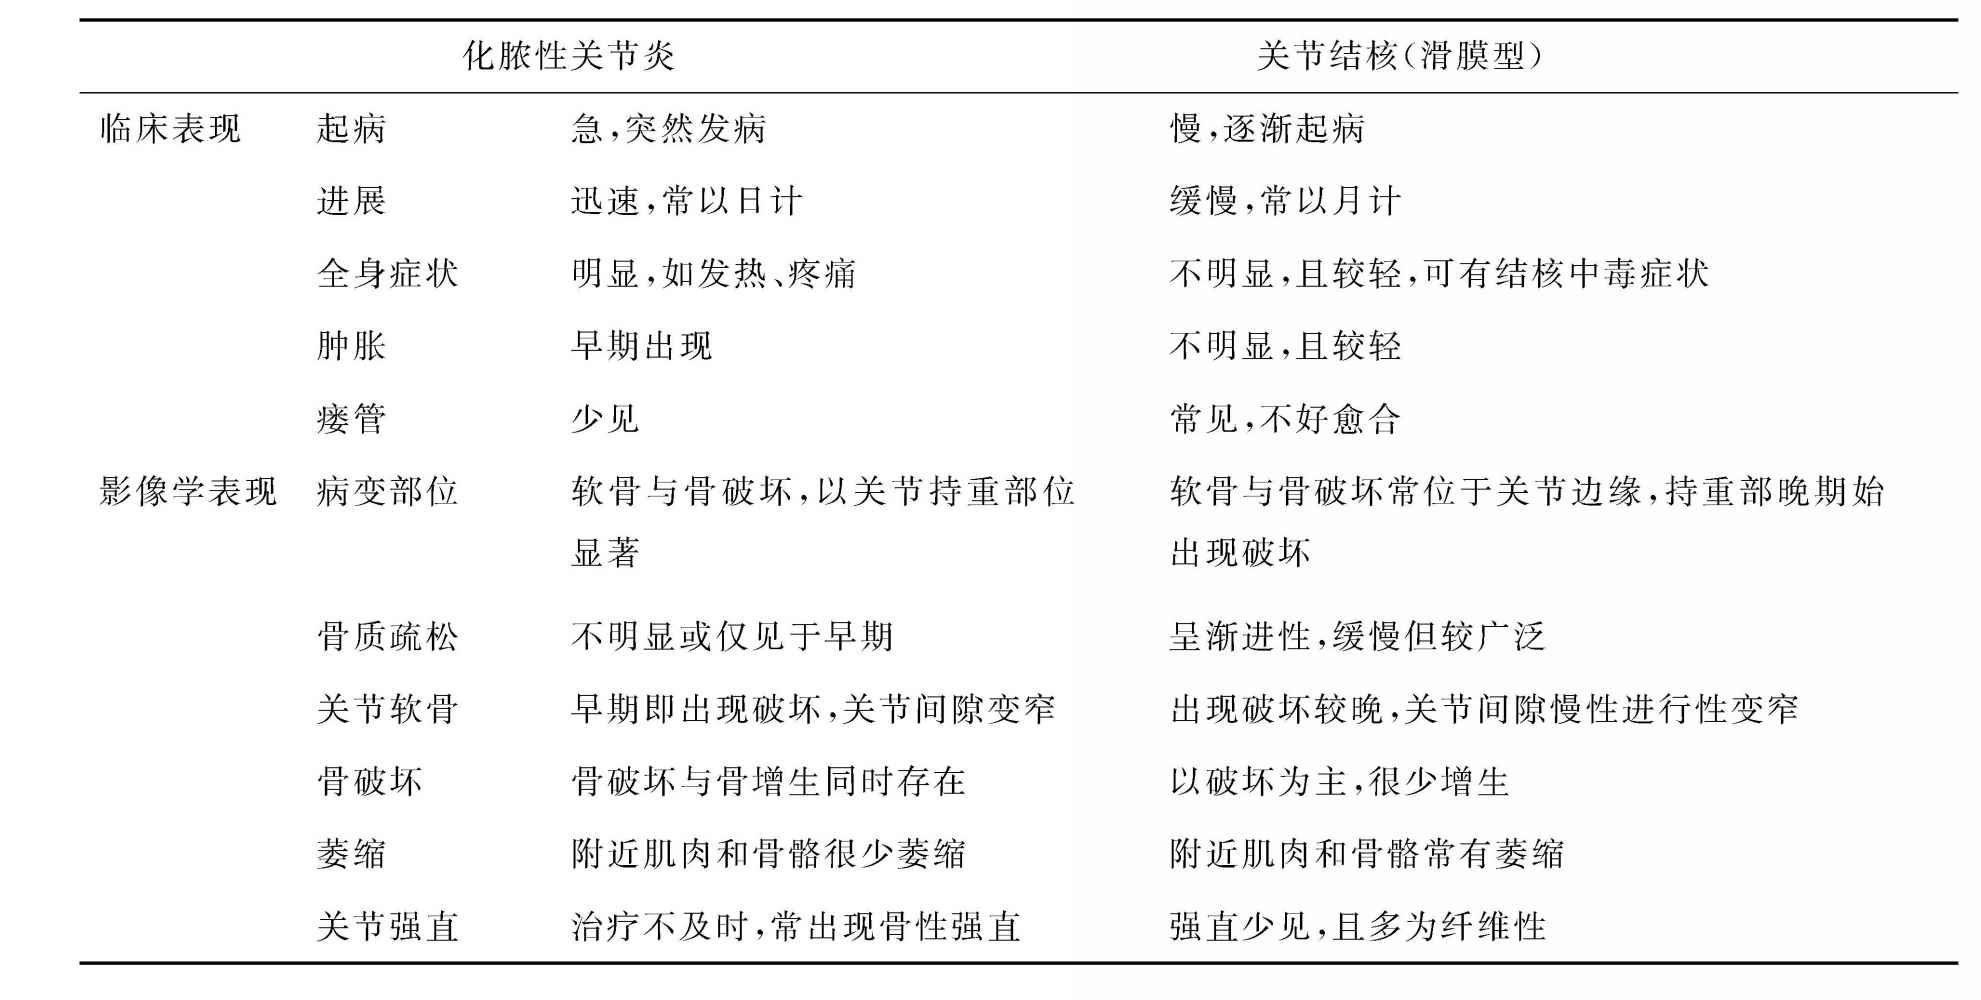
\includegraphics[width=\textwidth,height=\textheight,keepaspectratio]{./images/Image00433.jpg}
\end{table}

\section{骨肿瘤及肿瘤样病变}

\subsection{概述}

\subsubsection{临床表现}

①发病率:如良性骨肿瘤以骨软骨瘤最常见,骨瘤、软骨瘤、骨巨细胞瘤次之。恶性骨肿瘤以转移性多见,原发恶性骨肿瘤以骨肉瘤多见。②年龄:每个年龄期有好发某种骨肿瘤的倾向。③性别:以男性多见。④症状:主要是疼痛和出现肿块。⑤体征:良恶性有别。⑥实验室检查:良性骨肿瘤在血液、小便、骨髓等检查方面均为正常,恶性骨肿瘤常有异常改变。

\subsubsection{影像学分析}

①来源:从骨和软骨发生的肿瘤以良性居多,亦有恶性的;骨髓肿瘤多为恶性;来自骨膜的也大多为恶性。②部位:每一种骨肿瘤都有一定的好发部位。③数目:原发性骨肿瘤多为单发、良恶性均可;多发者以恶性多见如多发性骨髓瘤、转移瘤,良性者多发少见。④骨质改变:良性为扩张性压迫改变;恶性则为进行性破坏,常无明显膨胀。⑤骨膜反应:良性者多无,恶性多有。⑥软组织肿块:以恶性者多见。

\subsubsection{}

\begin{table}[htbp]
\centering
\caption{良恶性骨肿瘤的鉴别诊断}
\label{tab22-2}
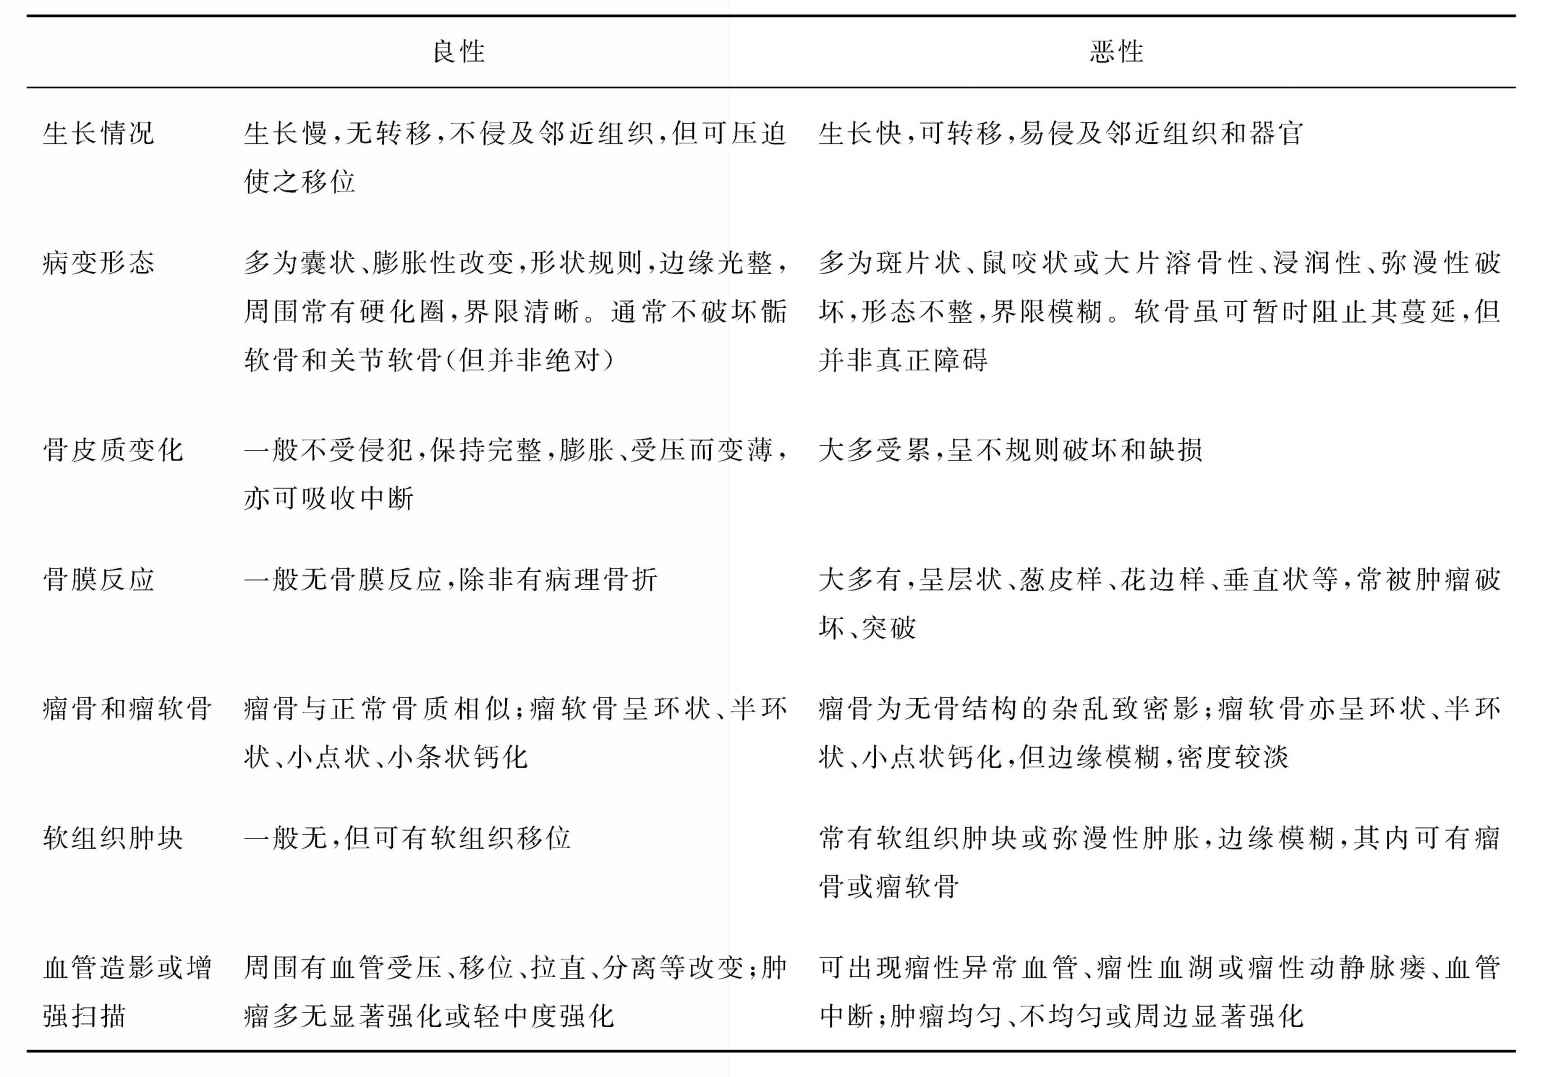
\includegraphics[width=\textwidth,height=\textheight,keepaspectratio]{./images/Image00434.jpg}
\end{table}

\subsection{骨瘤}

骨瘤系来源于膜内化骨的常见良性骨肿瘤,多发生于颅骨外板和鼻旁窦内,亦可见于舌、乳突、喉部、鞍结节等部位。其命名尚有争议。

\textbf{【病理】}
①致密型:整个瘤骨致密坚硬如象牙,故又称象牙质样骨瘤。②松质骨型:质地比较疏松或完全为疏松骨,环以菲薄骨壳,称为海绵样骨瘤。③混合型:具有以上两种成分,多表现为外部坚硬,而内部为松质骨。此外,病理学认为骨瘤以纤维骨化方式产生。因此,在其生长过程中,纤维组织和骨组织比例不同,有纤维瘤、骨化纤维瘤、纤维骨瘤和骨瘤之分。尚无恶变报道。

\textbf{【临床表现】}
多发病于30岁以下,男女比例约为1.4∶1。骨瘤一般待全身骨骼发育成熟后停止生长。常无症状,偶然发现。鼻窦口者可因继发鼻窦炎而出现相应症状。

\textbf{【CT表现】}
骨瘤为附着于颅骨内、外板或者突向鼻窦腔内的骨性突起。致密型似象牙质状;松质骨型结构疏松,又称疏松型。肿瘤一般不大,为1~2cm,较大者可同时累及内外板和板障。副鼻窦内可达6~7cm大小,可为多发(图\ref{fig22-16})。

\begin{figure}[!htbp]
 \centering
 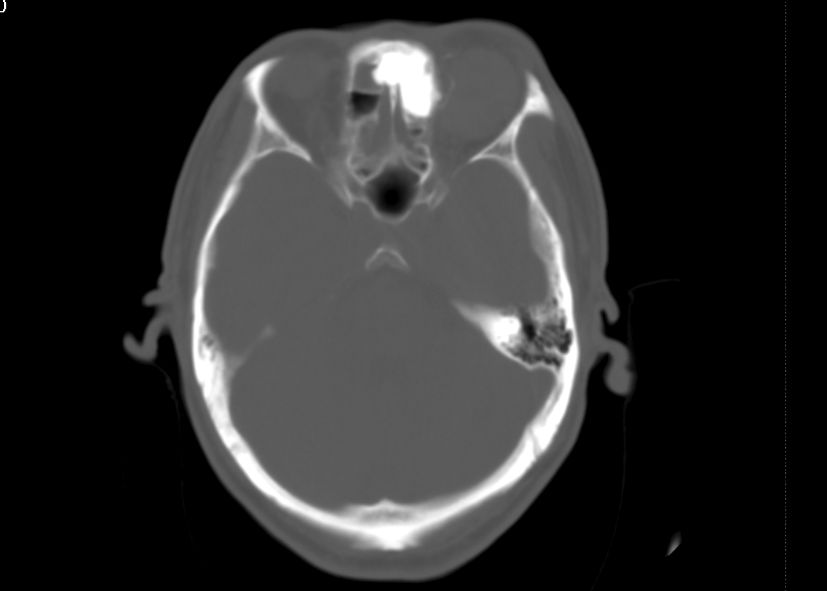
\includegraphics[width=.7\textwidth,height=\textheight,keepaspectratio]{./images/Image00435.jpg}
 \captionsetup{justification=centering}
 \caption{筛窦骨瘤\\{\small 前组筛窦区可见致密骨密度灶,以左侧为主}}
 \label{fig22-16}
  \end{figure} 

Gardner(加德纳)综合征亦称家族性息肉症,系骨瘤合并结肠息肉病,以及软组织肿瘤(如脂肪瘤、纤维瘤、皮样囊肿等),为家族性常染色体显性遗传性疾病。

此外,四肢骨瘤可分为以下两型:①内生骨瘤:系起源于髓腔或骨内膜的良性肿瘤,有人称为“骨岛”,很少见。其特点是位于松质骨或髓腔,其余表现同骨瘤,发病部位不定。②骨旁骨瘤:系发生于四肢骨骨旁的骨瘤,少见。以双股骨远端后多见,其次为肱骨干。术后可复发或恶变为骨旁骨肉瘤。瘤体边缘可不规整,但清晰。骨皮质无侵蚀破坏征象。肿瘤多与骨皮质紧密相连,可生长巨大。

\textbf{【鉴别诊断】}
应注意与额骨内板增生症相鉴别。额骨内板增生症多见于40岁以上女性,绝大多数为绝经后老年妇女。可产生一些症状如头痛、肥胖、多毛、男性化及高血压,少数合并神经精神症状如迟钝、痴呆、抑郁、癔病,以及肢端肥大症、毒性甲状腺肿、糖尿病等。影像学表现额骨最为常见,少数累及顶骨前部。其特征性表现为颅骨内板和板障骨质增生,逐渐发展,双侧对称或基本对称。按增生形态可分为梭形或波浪状,按范围可分为局限性或弥漫性。增生最厚可达2cm,外板不受侵,亦不累及眶顶,蝶鞍正常。

骨瘤一般呈内板或外板的丘状骨性突起,多为致密型,而密度高于额骨内板增生症,且骨瘤几乎没有双侧对称性发生者。

此外,还有板障型脑膜瘤的报道,示脑膜肿瘤改变不明显,而颅骨内外板呈花边样、锯齿样明显增厚,板障变窄,应注意与骨瘤、额骨内板增生症等相鉴别。

\subsection{骨软骨瘤}

本病是软骨化骨中最常见的肿瘤,可单发或多发。主要发生于软骨内化骨的干骺端,以膝部多见,亦可见于扁骨及不规则骨。

\textbf{【病理】}
肿瘤大小不一,为1~10cm,沿肌肉牵拉方向生长。由骨性基底、软骨帽和纤维包膜3部分构成。根据骨性基底部形态不同,可分为带蒂和广基两种。软骨帽外为纤维膜,纤维膜深层可产生透明软骨组织,恶变一般由深层开始。单发者恶变占1%,多发者占11%~25%。此外,发生于骨盆、肩胛骨、脊柱和肋骨者恶变机会较多。较大的骨软骨瘤在顶部可有滑囊形成,内含滑液,可发生滑囊炎和滑膜骨软骨瘤病。

\textbf{【临床表现】}
好发于10~30岁,男女发病率相近,长骨干骺端为好发部位。早期无症状,肿瘤较大时可有轻压痛和畸形,并可有关节活动障碍。骨软骨瘤于成年后又突然加速生长,疼痛加剧,提示有恶变可能。

\textbf{【CT表现】}
①肿瘤的骨体:其皮质、松质与正常骨质相延续,与骨相连处呈蒂状或宽基底状。②软骨钙化:呈环形钙化,重叠在一起可类似菜花状。③肿瘤顶端的软骨帽:CT片可借助周围软组织等观察其厚度。

巨大菜花样骨软骨瘤表示肿瘤生长活跃,生长活跃的骨软骨瘤常在某一局部发生恶变。其恶变的影像学征象有:①肿瘤表面分叶状或环形钙化带突然中断不连续。②钙化带中断或消失的部位出现软组织肿块或软骨帽明显增厚。③该处的钙化带密度减低,软组织肿块内出现散在的斑点状或低密度钙化环。④大部钙化带模糊、密度减低,局部骨皮质发生破坏或出现骨膜反应。⑤瘤体内发生象牙质样瘤骨。

\subsection{长骨良性囊状肿瘤和肿瘤样病变}

长骨的良性囊状骨肿瘤和肿瘤样病变种类繁多,其诊断应以平片为主,但CT检查可提供更多的影像学征象甚至特征(图\ref{fig22-17}~图\ref{fig22-20})。螺旋CT三维重建的应用对其诊断有特殊的价值。本书对长骨良性囊状肿瘤和肿瘤样病变不作繁述,见表\ref{tab22-3}。

\begin{figure}[!htbp]
 \centering
 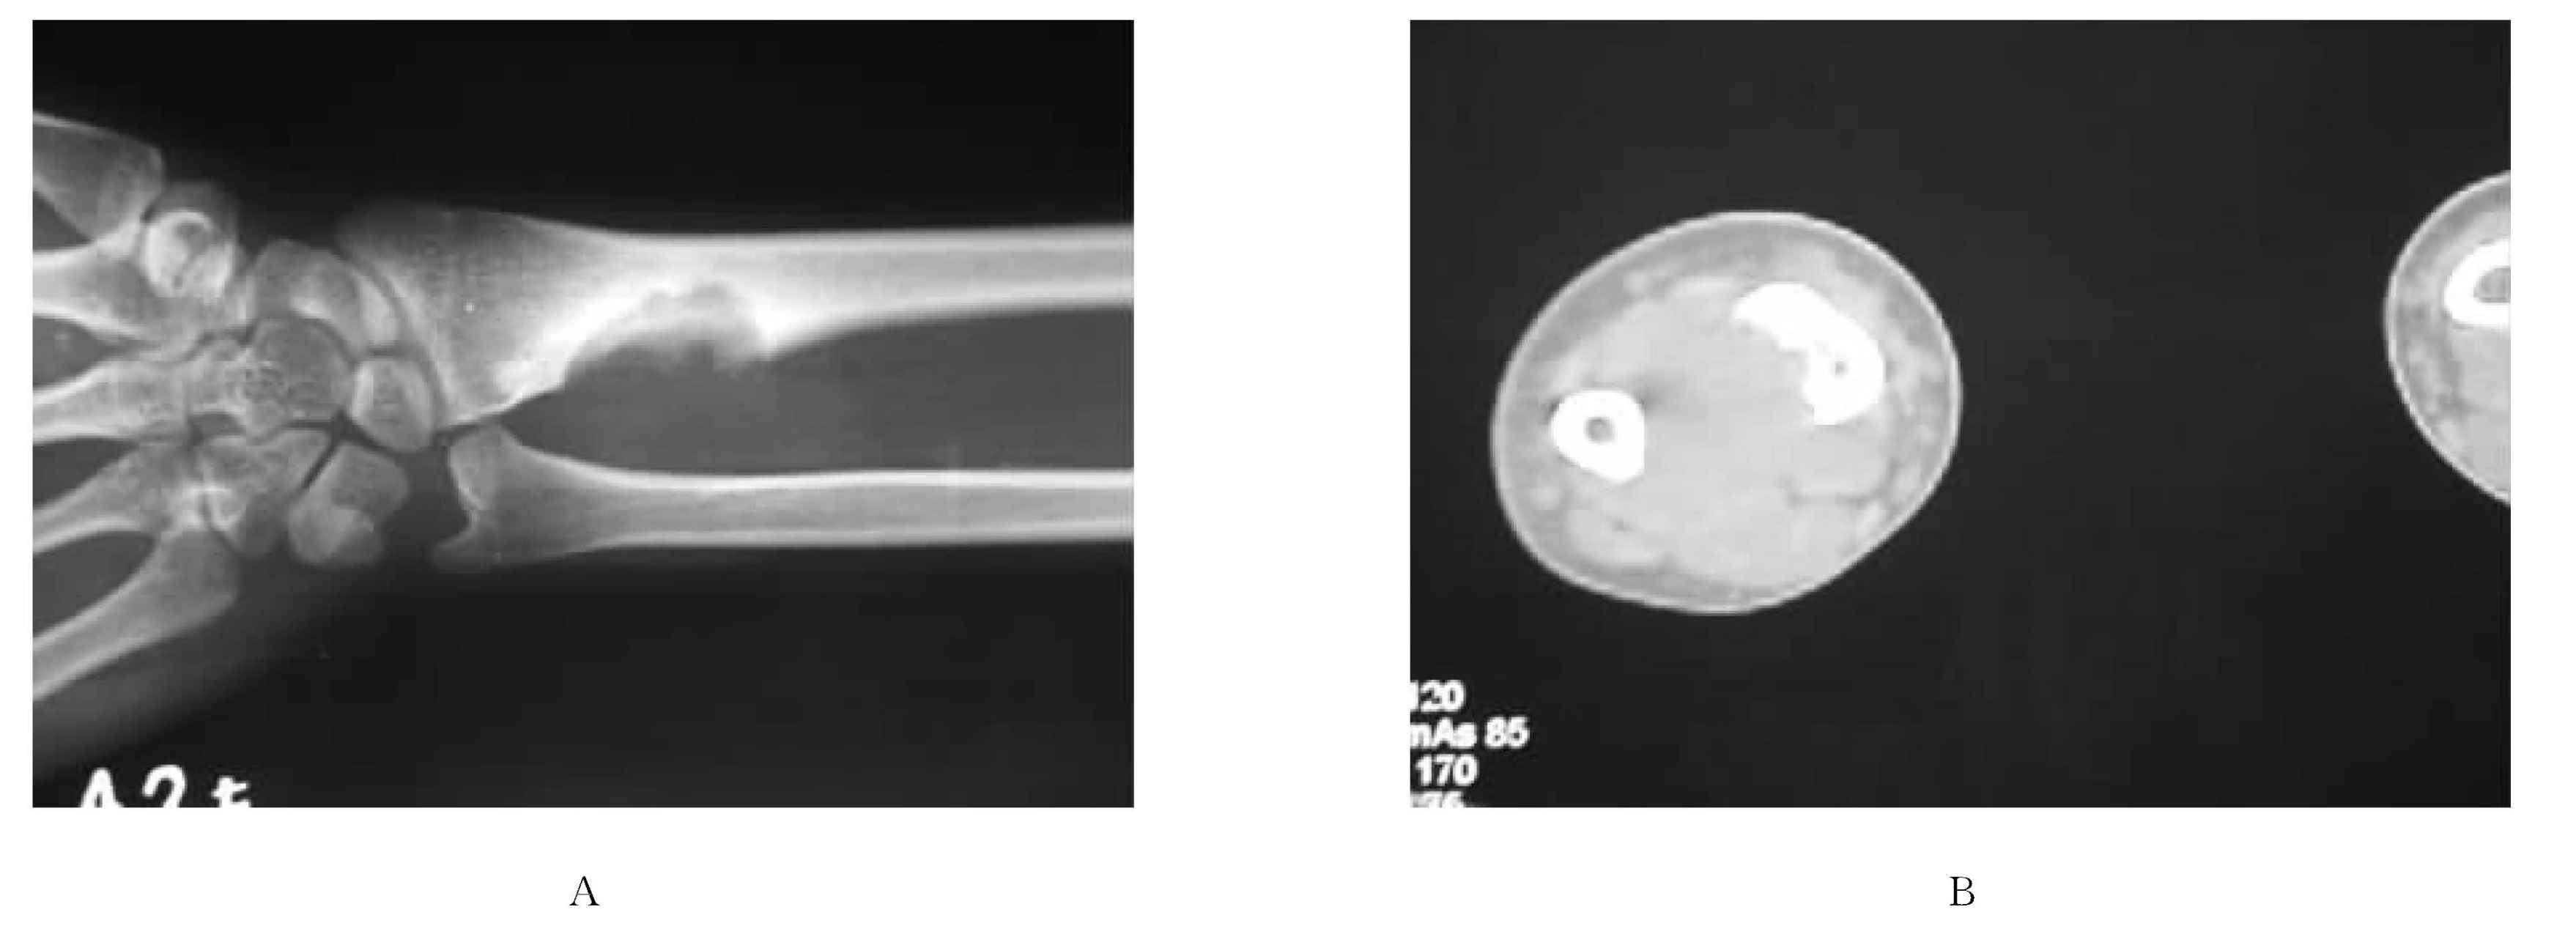
\includegraphics[width=.7\textwidth,height=\textheight,keepaspectratio]{./images/Image00436.jpg}
 \captionsetup{justification=centering}
 \caption{软骨黏液样纤维瘤\\{\small 右侧桡骨远端有偏心性、分叶状低密度区,其邻近骨质硬化明显,局部有软组织块}}
 \label{fig22-17}
  \end{figure} 

\begin{figure}[!htbp]
 \centering
 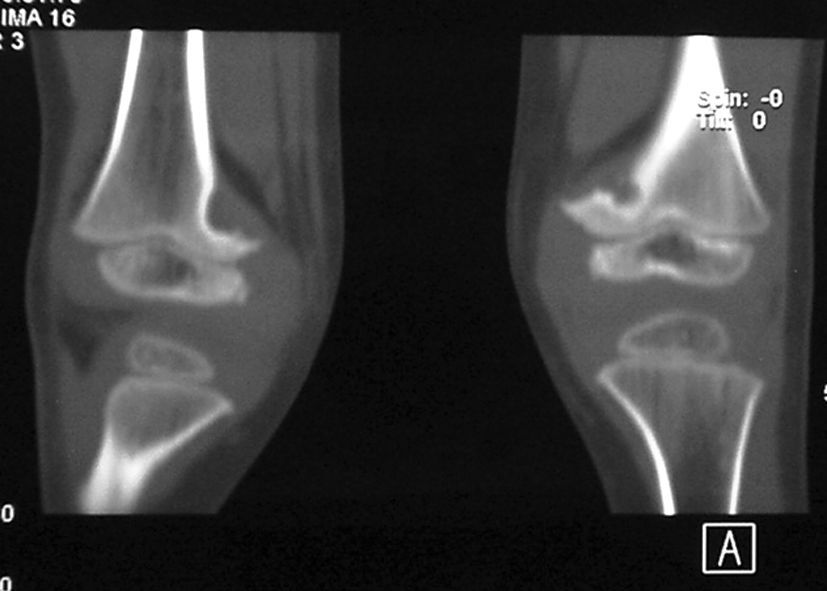
\includegraphics[width=.7\textwidth,height=\textheight,keepaspectratio]{./images/Image00437.jpg}
 \captionsetup{justification=centering}
 \caption{纤维性骨皮质缺损\\{\small 左右股骨远端局部骨皮质呈波浪状凹陷缺损,边缘硬化,无软组织块}}
 \label{fig22-18}
  \end{figure} 

\begin{figure}[!htbp]
 \centering
 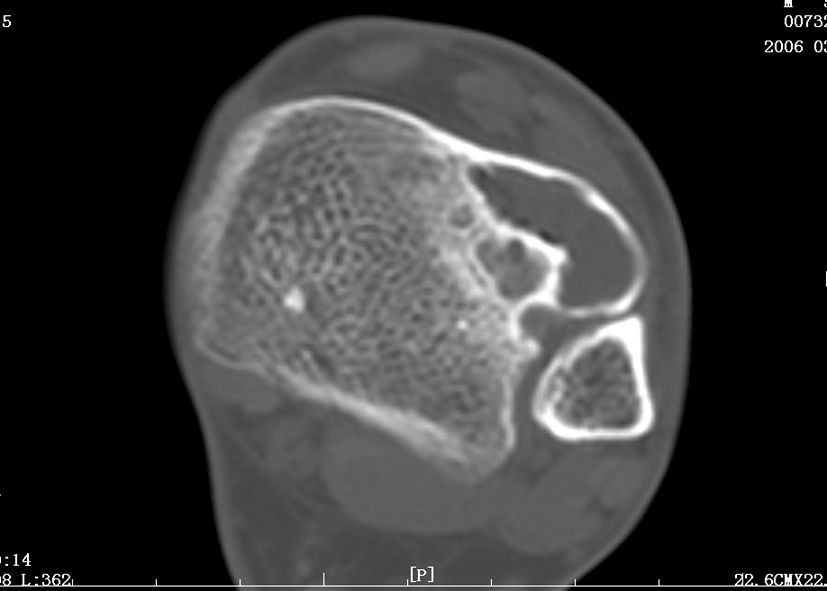
\includegraphics[width=.7\textwidth,height=\textheight,keepaspectratio]{./images/Image00438.jpg}
 \captionsetup{justification=centering}
 \caption{邻关节囊肿\\{\small 左侧胫骨远端邻近关节的多房囊状低密度灶,偏心分布,边缘薄层硬化,并有骨嵴}}
 \label{fig22-19}
  \end{figure} 

\begin{figure}[!htbp]
 \centering
 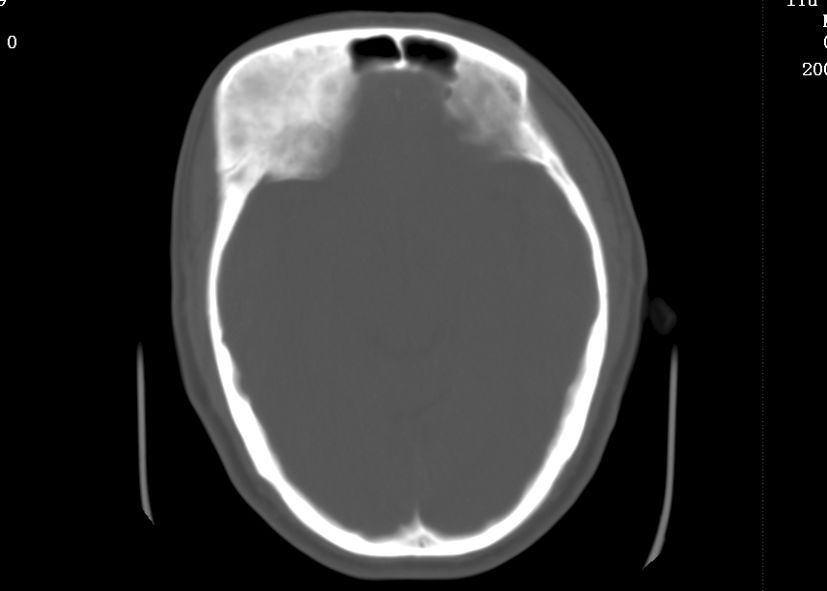
\includegraphics[width=.7\textwidth,height=\textheight,keepaspectratio]{./images/Image00439.jpg}
 \captionsetup{justification=centering}
 \caption{骨纤维异常增殖症\\{\small 额骨右侧有大片状磨玻璃样高密度区,其内有多个囊样稍低密度区,界限欠清晰}}
 \label{fig22-20}
  \end{figure} 

\begin{figure}[!htbp]
 \centering
 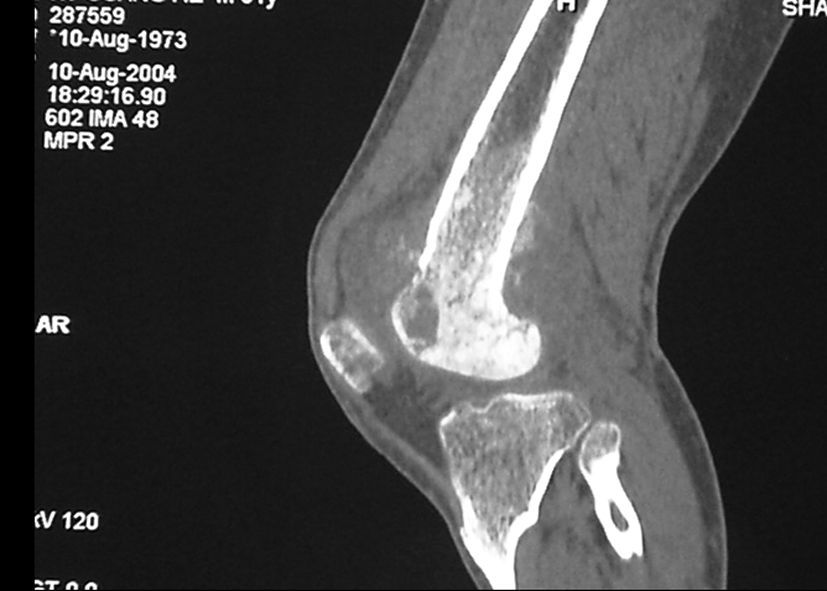
\includegraphics[width=.7\textwidth,height=\textheight,keepaspectratio]{./images/Image00440.jpg}
 \captionsetup{justification=centering}
 \caption{骨肉瘤\\{\small 右侧股骨远端有溶骨性骨质破坏表现,并可见斑片状不规则瘤骨及不规则软组织块}}
 \label{fig22-21}
  \end{figure} 

\begin{longtable}{c}
  \caption{长骨良性囊状病变的诊断与鉴别诊断}
  \label{tab22-3}\\
  \endfirsthead
  \caption[]{长骨良性囊状病变的诊断与鉴别诊断}
  \endhead
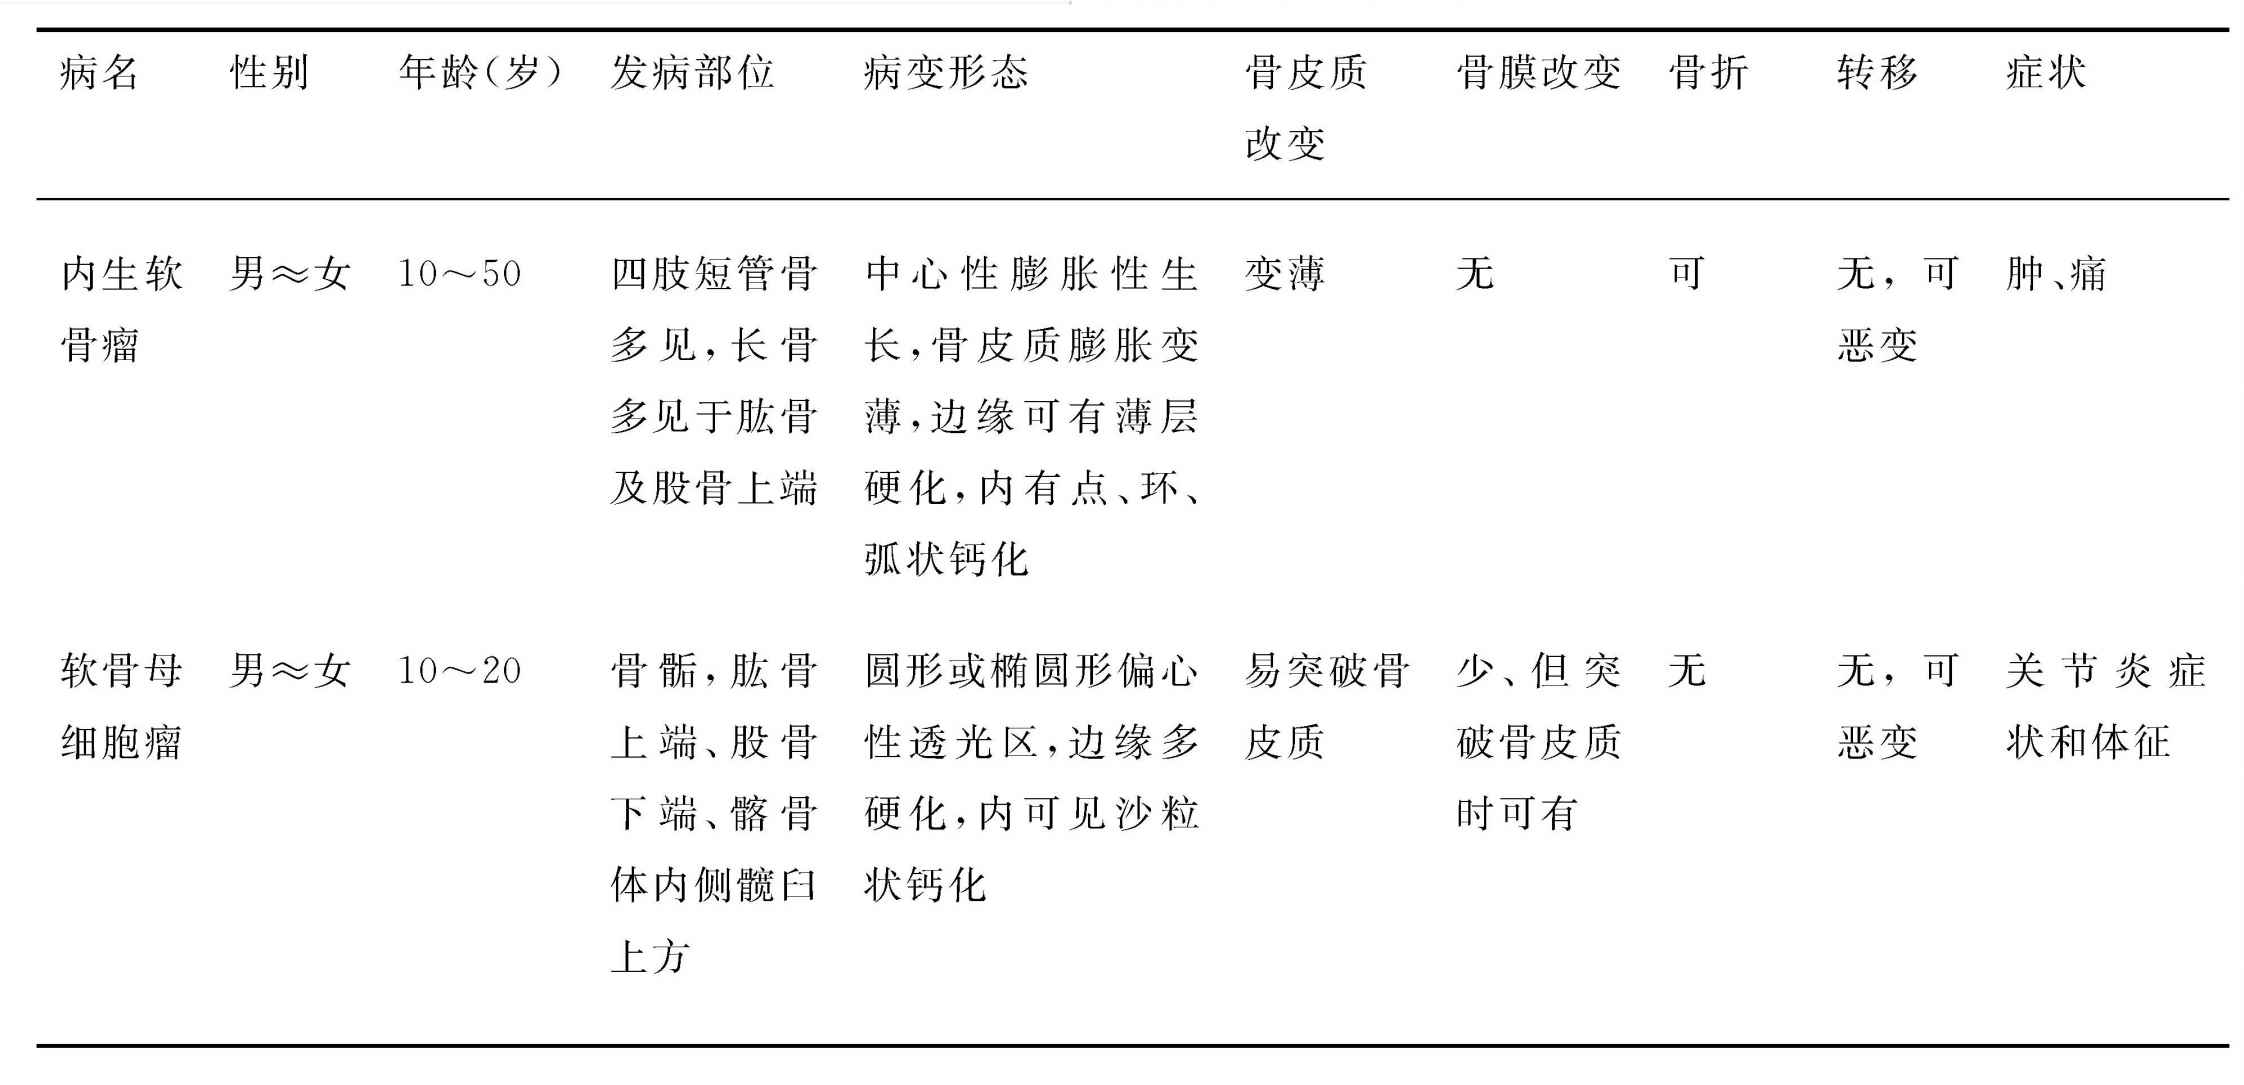
\includegraphics[width=\textwidth,height=\textheight,keepaspectratio]{./images/Image00441.jpg}\\
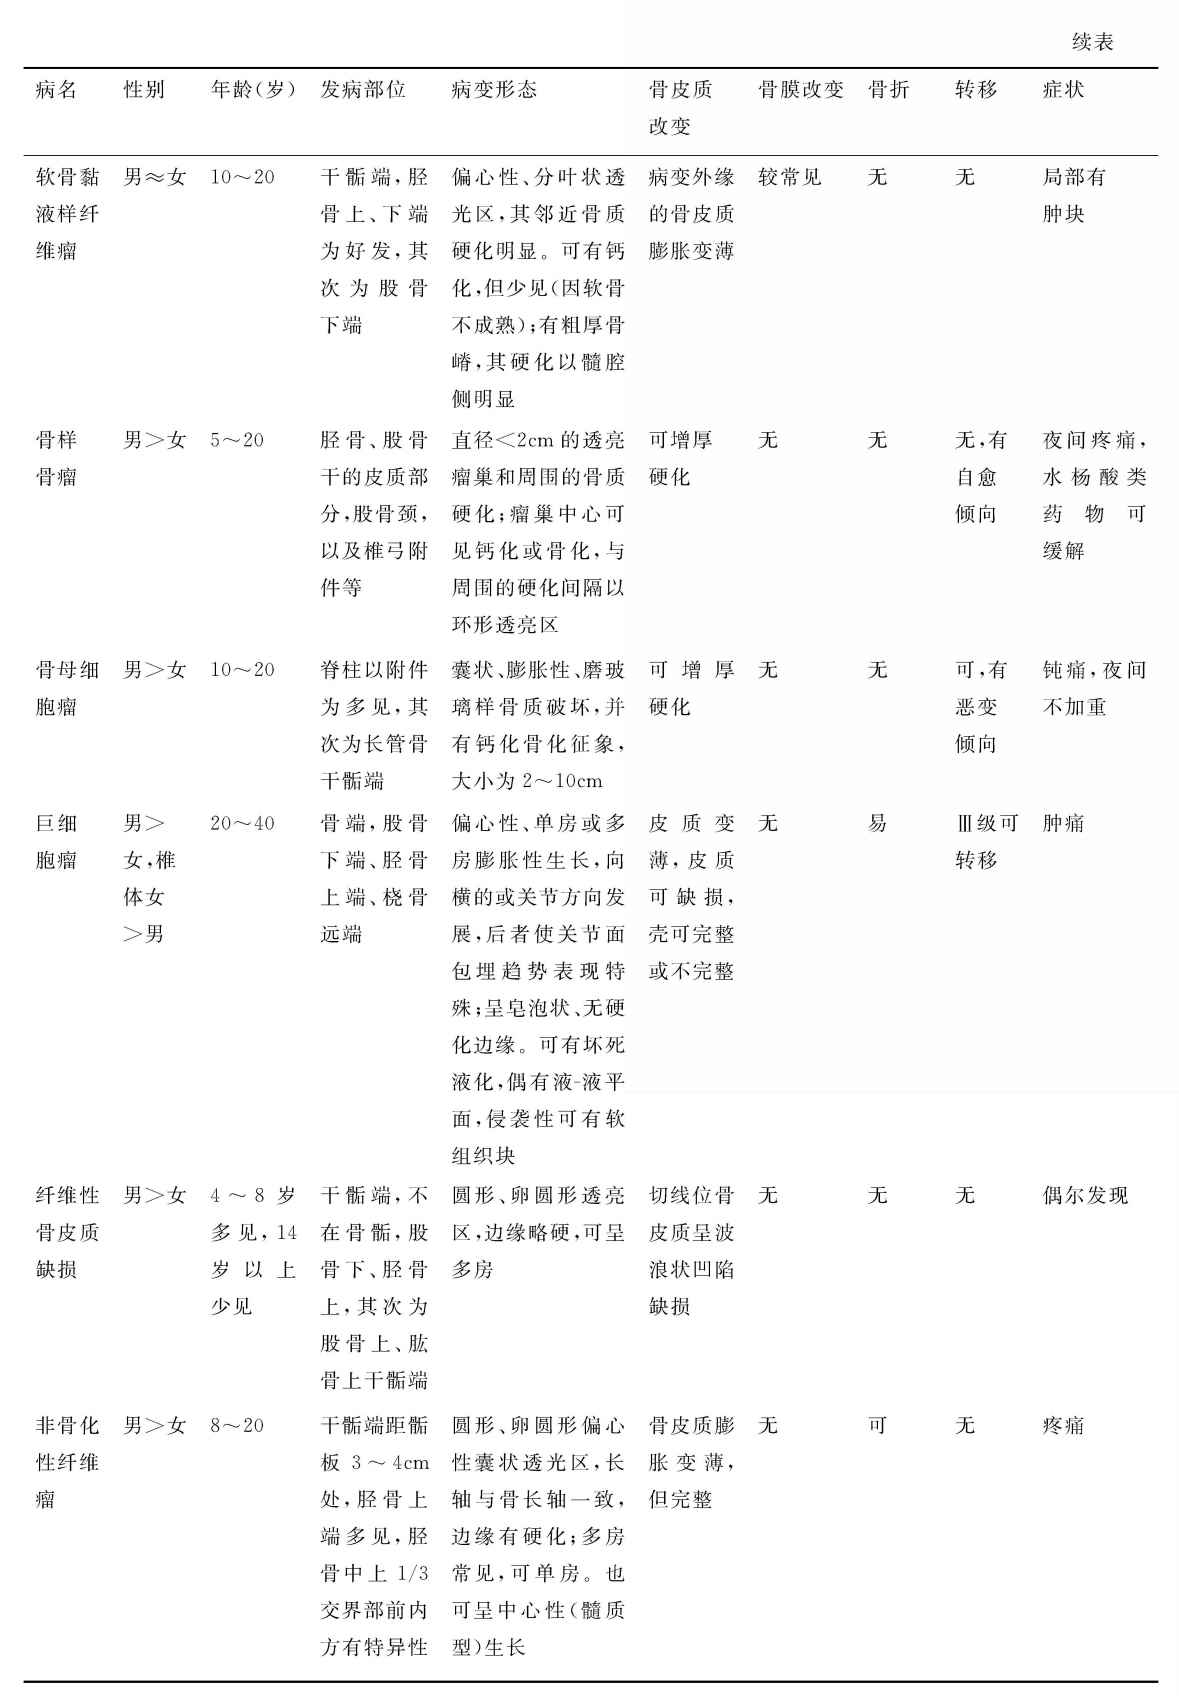
\includegraphics[width=\textwidth,height=\textheight,keepaspectratio]{./images/Image00442.jpg}\\
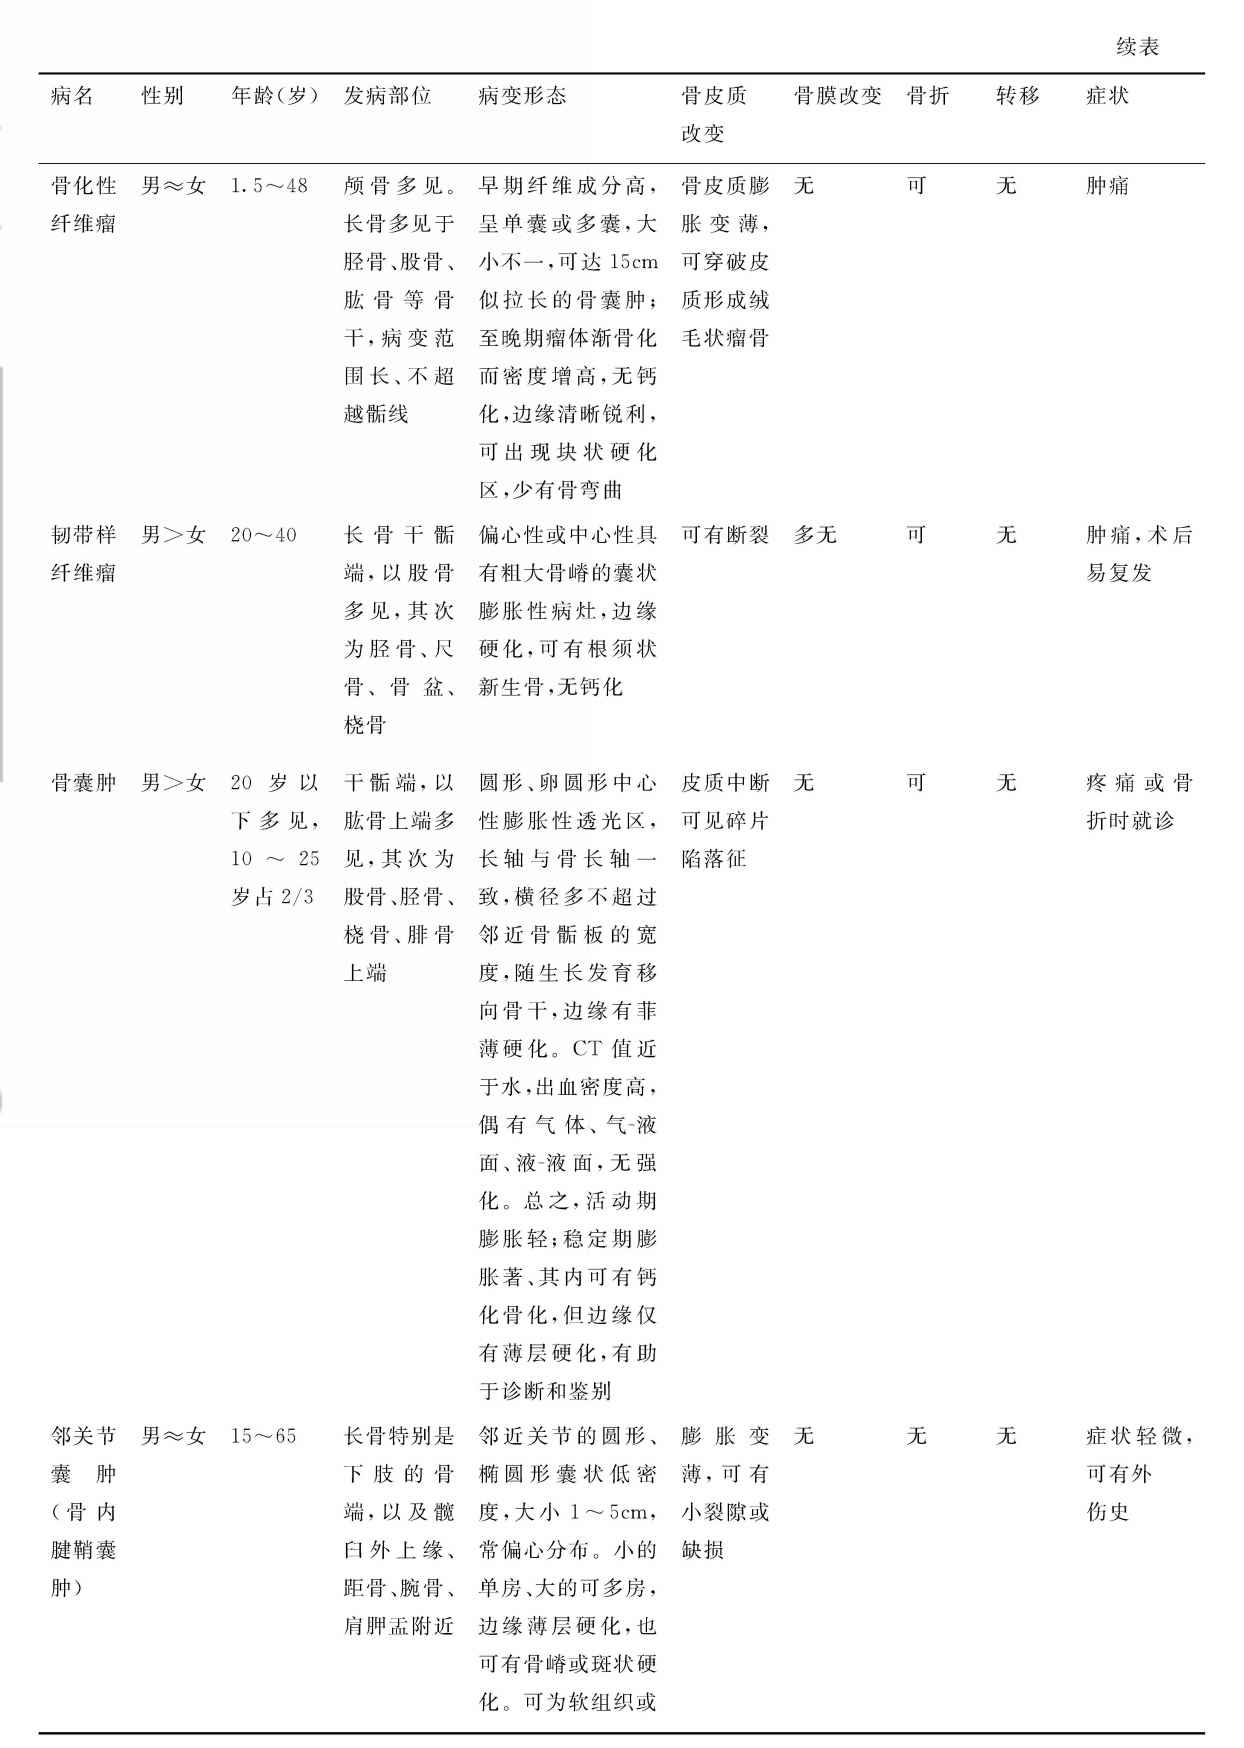
\includegraphics[width=\textwidth,height=\textheight,keepaspectratio]{./images/Image00443.jpg}\\
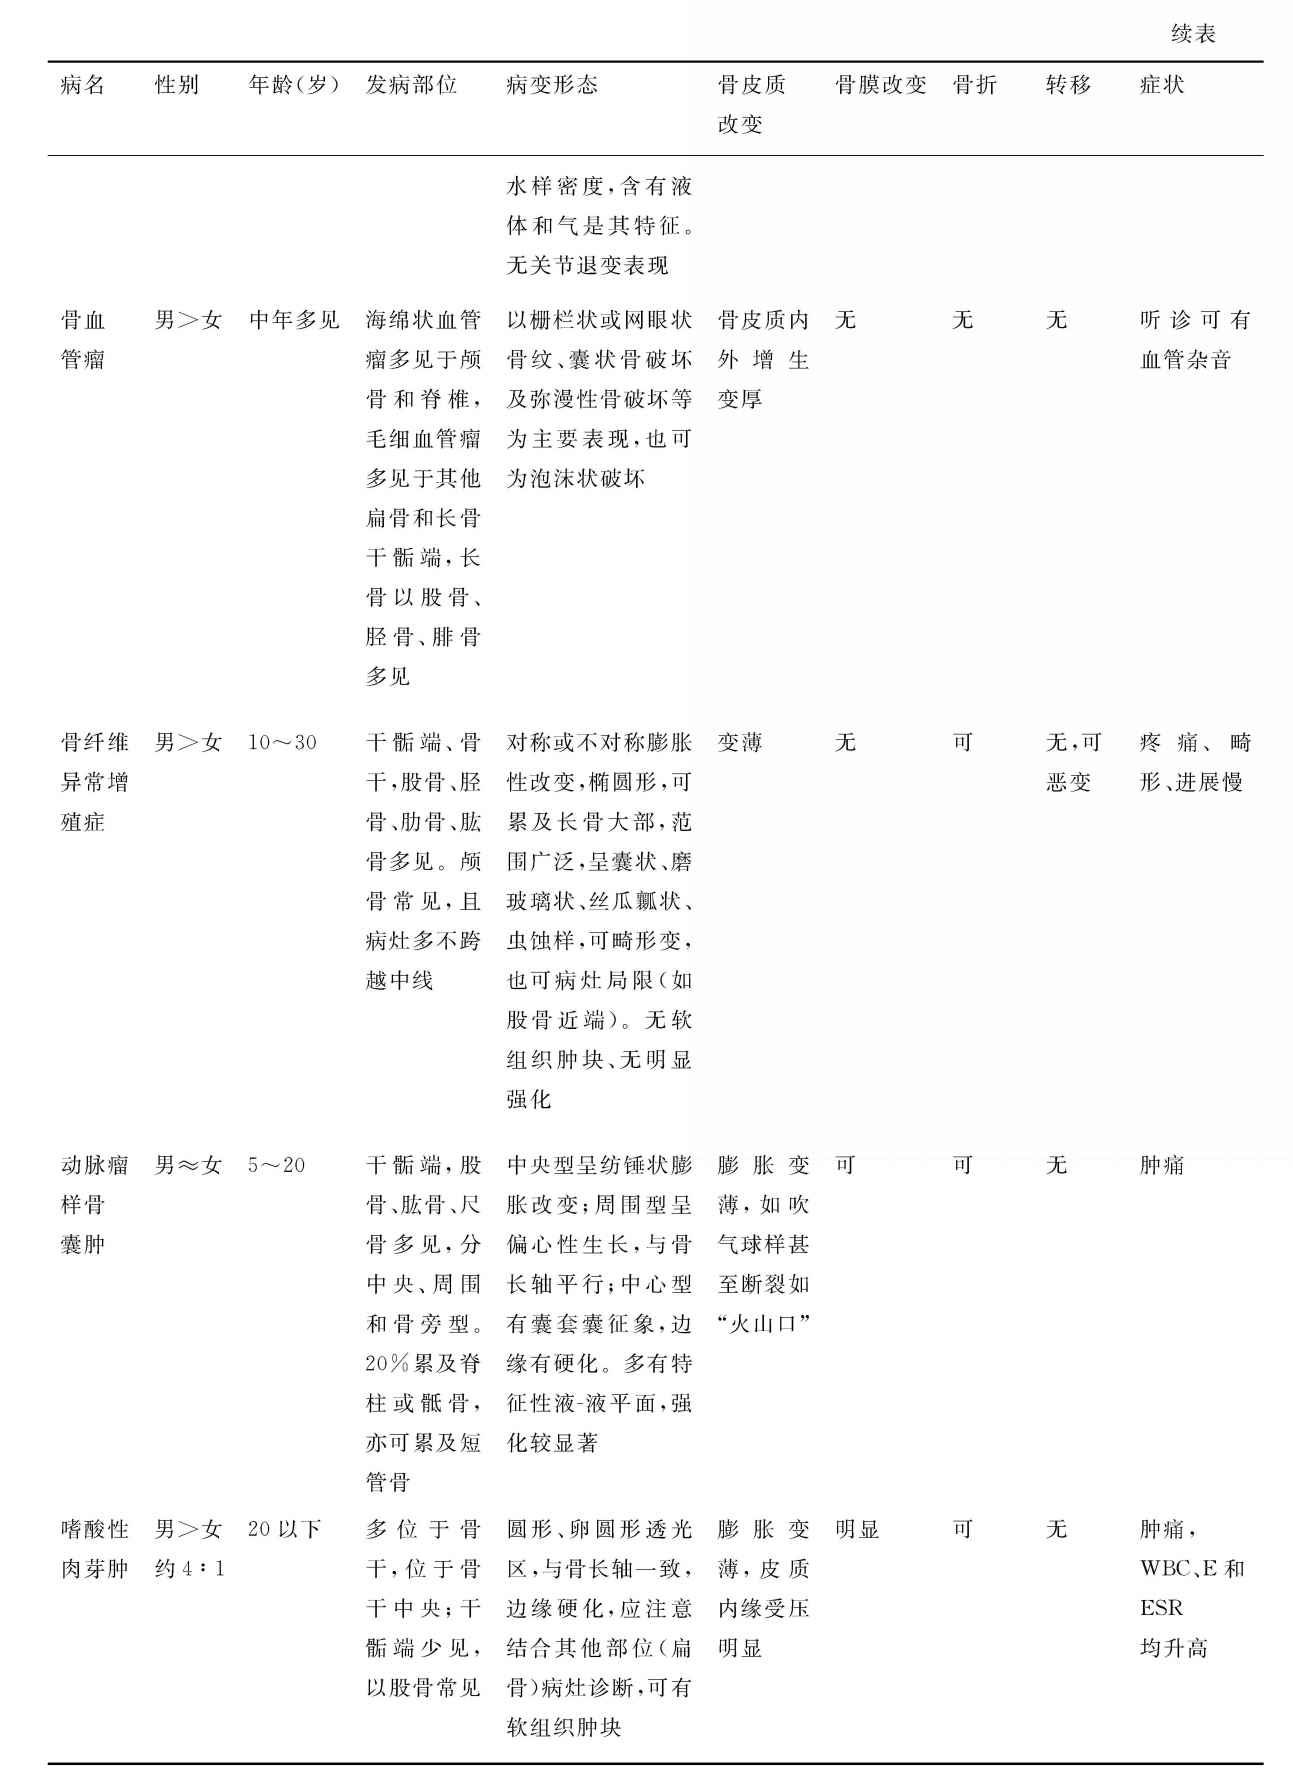
\includegraphics[width=\textwidth,height=\textheight,keepaspectratio]{./images/Image00444.jpg}
\end{longtable}



\subsection{原发性恶性骨肿瘤}

CT检查有利于显示恶性肿瘤的生长情况、骨质破坏范围和形态,尤其有利于显示软组织肿块(图\ref{fig22-21})。增强扫描可显示与邻近血管的关系,甚至可以显示肿瘤血管,是平片所不及的。几种常见的原发性恶性骨肿瘤的诊断要点见表\ref{tab22-4}。

\begin{table}[htbp]
\centering
\caption{几种原发性恶性骨肿瘤的诊断要点}
\label{tab22-4}
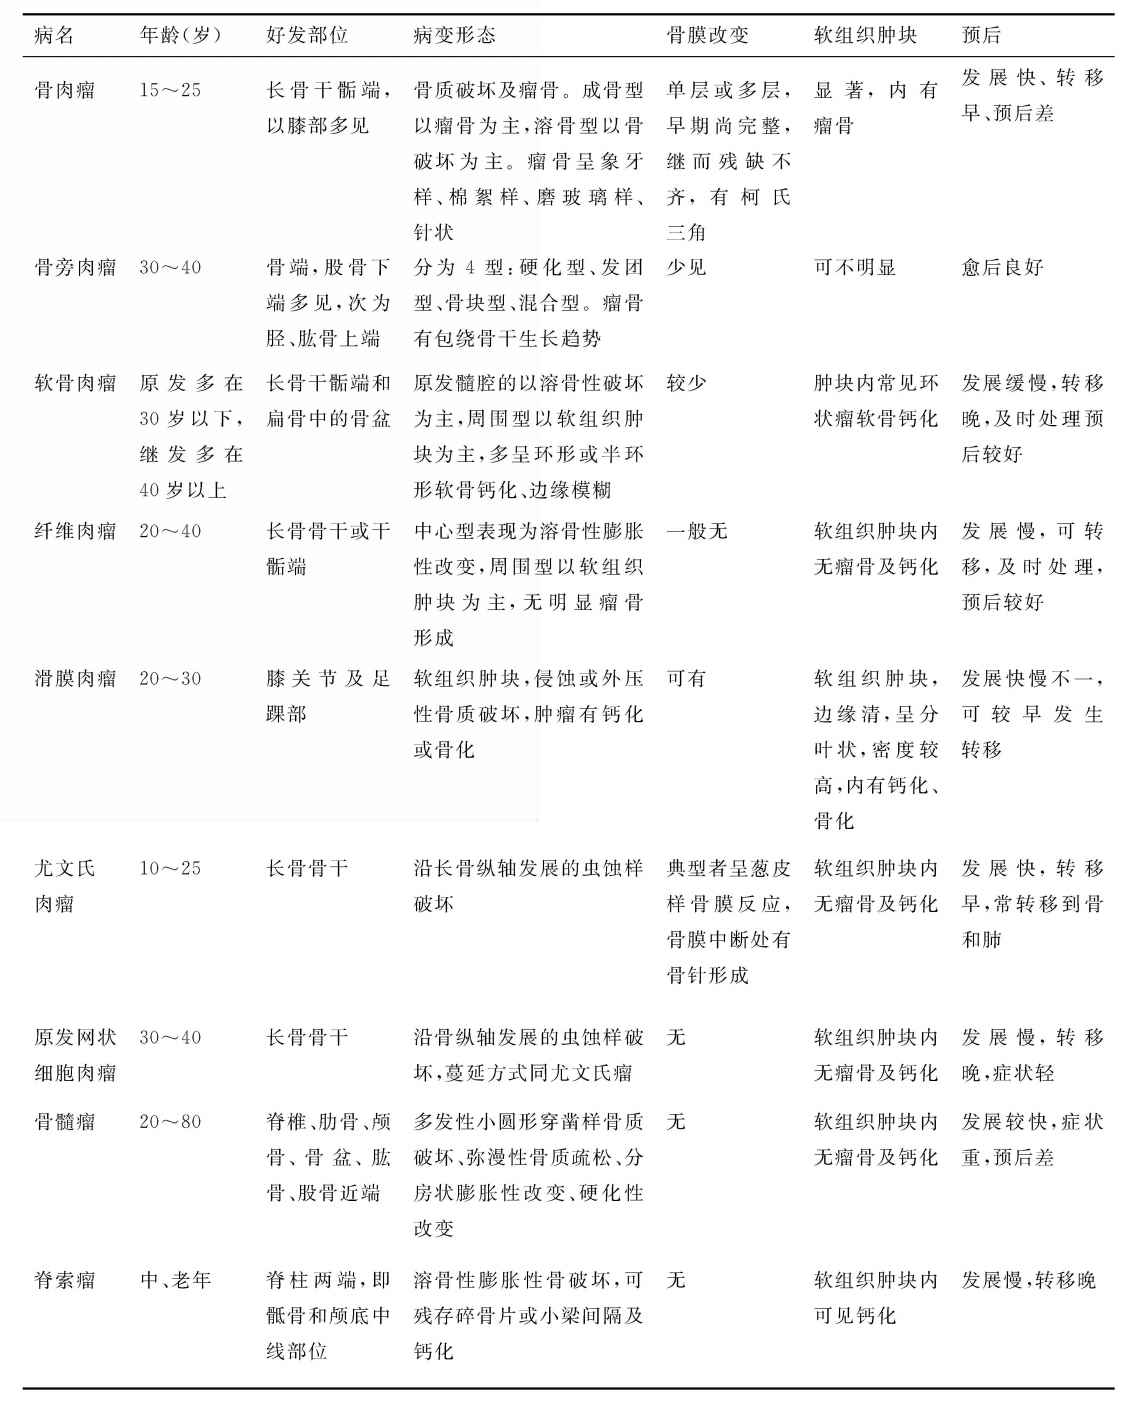
\includegraphics[width=\textwidth,height=\textheight,keepaspectratio]{./images/Image00445.jpg}
\end{table}

\subsection{骨转移瘤}

\textbf{【病因病理】}
几乎所有的癌和肉瘤均可转移至骨骼,但以癌为多见,其中以乳癌、鼻咽癌、肺癌、甲状腺癌、肾癌、宫颈癌、卵巢癌、前列腺癌、食管癌、胃癌、肠癌及肝癌等常见。骨的原发肿瘤除尤文氏瘤可有骨转移外,其他少见。在儿童中以神经母细胞瘤多见。

肿瘤转移至骨骼可由血行、淋巴或者直接蔓延3种途径。其中主要通过血行转移。血行转移的途径如下:①腔静脉型;②门静脉型;③肺静脉型;④脊柱静脉型:脊柱静脉系统无静脉瓣,且与胸、腹、盆腔静脉丛相交通,随胸、腹腔压力增高,肿瘤栓子可直接进入该系统;⑤选择性转移:即某些原发肿瘤栓子经血行能够选择与原发肿瘤相同的环境停留下来,如骨髓瘤的转移即属此类。

任何骨骼均可发生骨转移瘤,但黄骨髓中没有血窦系统,小动脉和毛细血管完整,故很少发生转移。成年人脊柱、骨盆、颅骨、肋骨、股骨上端和肱骨终生为红骨髓,故易发生骨转移。病理上可分为溶骨型、成骨型和混合型转移。

\textbf{【临床表现】}
主要是疼痛,多为持续性、夜间加重,有时可出现肿块、病理骨折和压迫症状。实验室检查:成骨性转移者碱性磷酸酶升高、血清钙磷正常或偏低;溶骨性转移者血清钙磷常有轻度增高;前列腺癌转移者酸性磷酸酶增高。此外,还有体重减轻、贫血、发热和血沉增快等。

\textbf{【CT表现】}

1.溶骨型:最常见,多为甲状腺癌、肾癌、肺癌、宫颈癌及消化道癌肿。前列腺癌的骨转移虽多为成骨性,但亦有溶骨性者。也就是说,几乎所有的恶性肿瘤均可发生溶骨性转移。常为多发,单发少见。表现为受累骨骼呈点状、斑片状、虫蚀状骨质破坏,边缘不规则,随病变进展破坏区可融合成大片状(图\ref{fig22-22}A~C)。除非合并病理骨折,很少有骨膜反应,常有软组织肿块。

2.成骨型:较溶骨型少见。绝大多数来自前列腺癌,占80%~90%以上,少数为乳癌、膀胱癌、鼻咽癌及肺癌等,一般为多发性病灶。多在骨外形无何改变的情况下出现片状、圆形、椭圆形致密影,边缘不整;亦可呈地图状、小结节、棉絮状高密度灶(图\ref{fig22-22}D)。一般无软组织肿块,也少有骨膜反应。



\begin{figure}[!htbp]
 \centering
 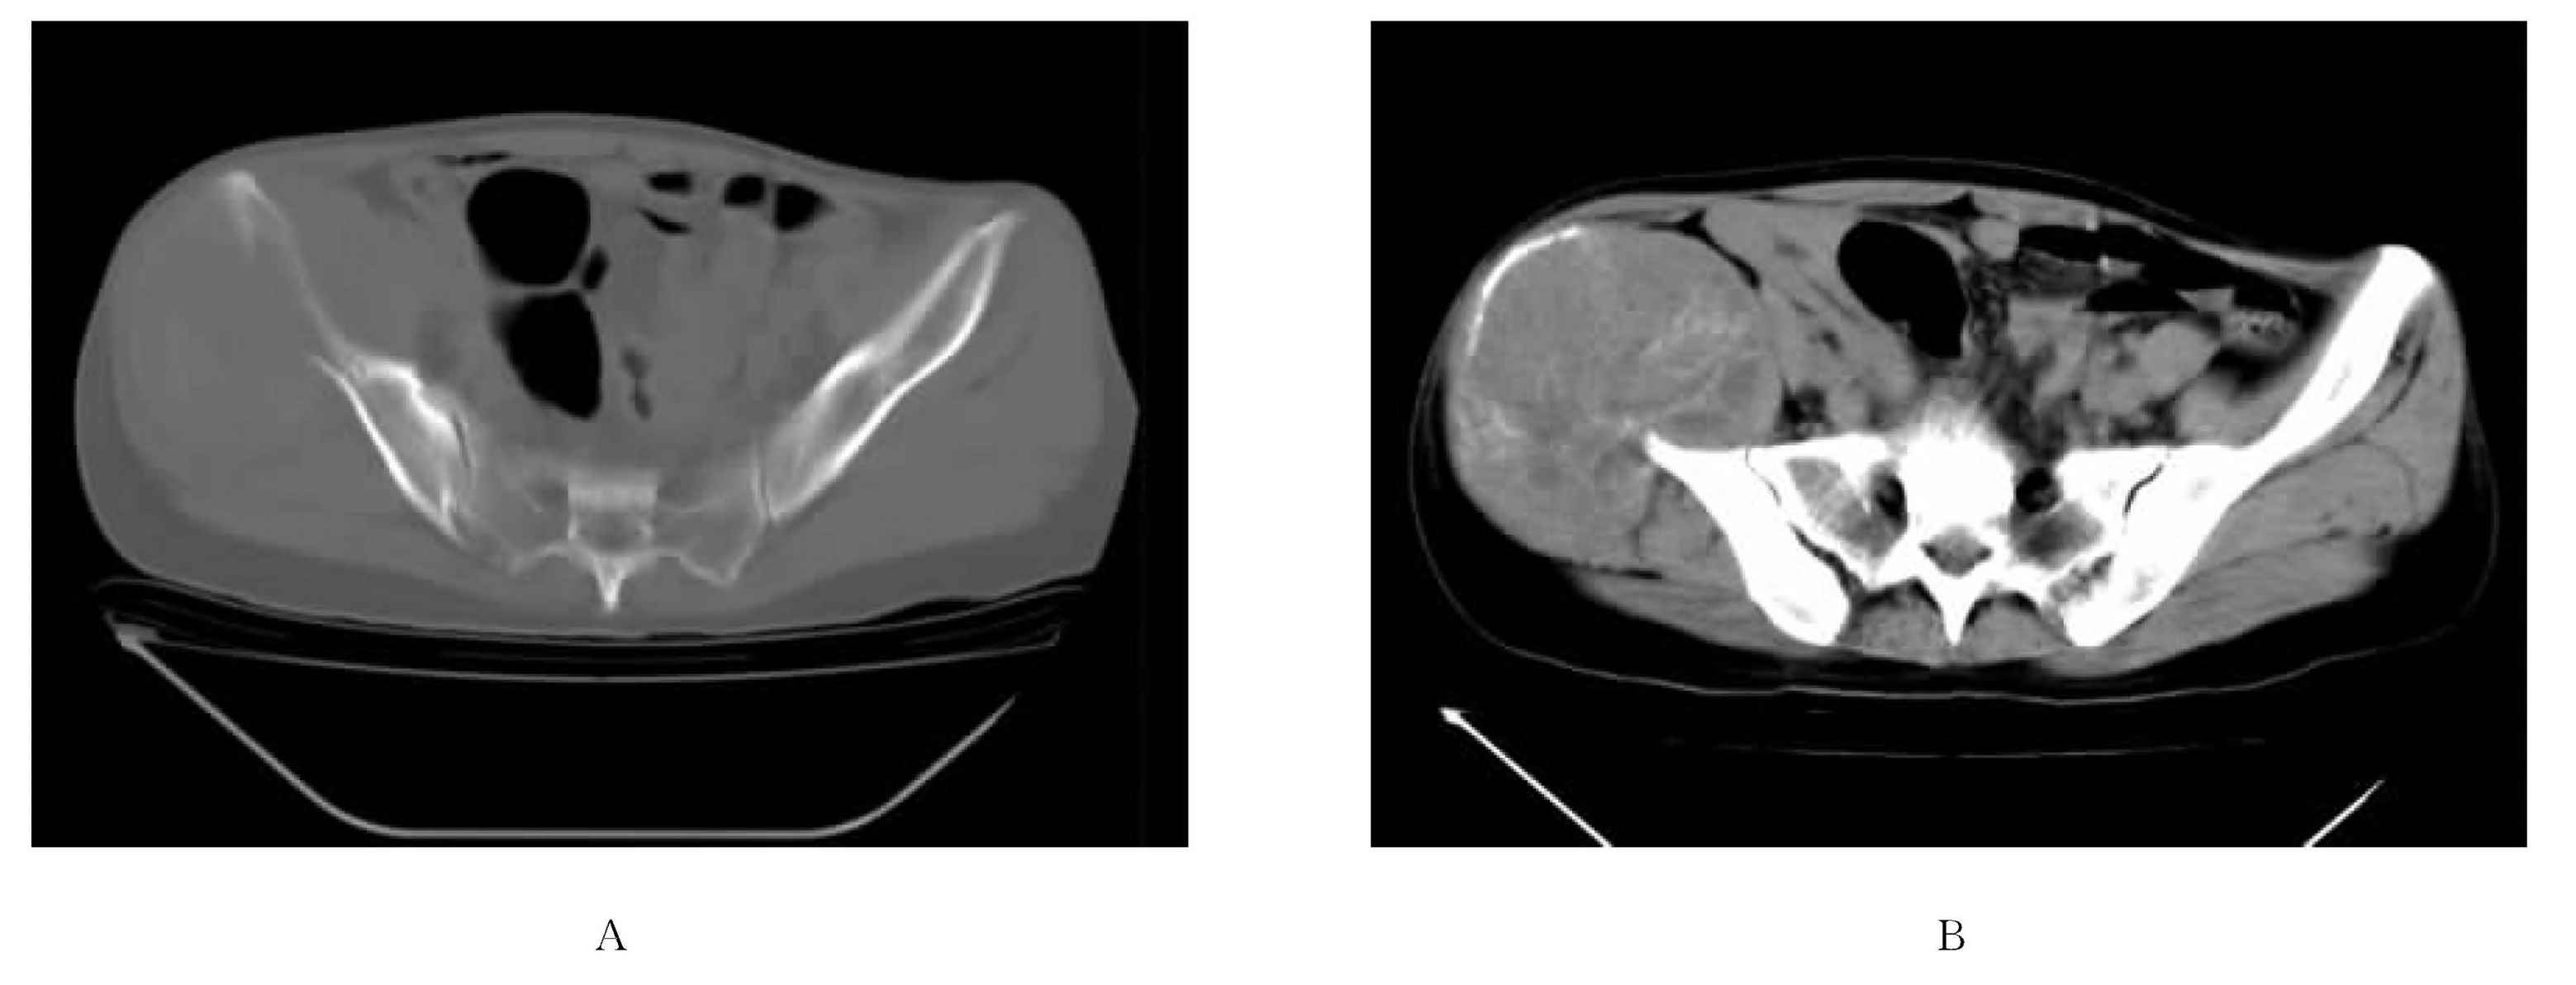
\includegraphics[width=.7\textwidth,height=\textheight,keepaspectratio]{./images/Image00446.jpg}
 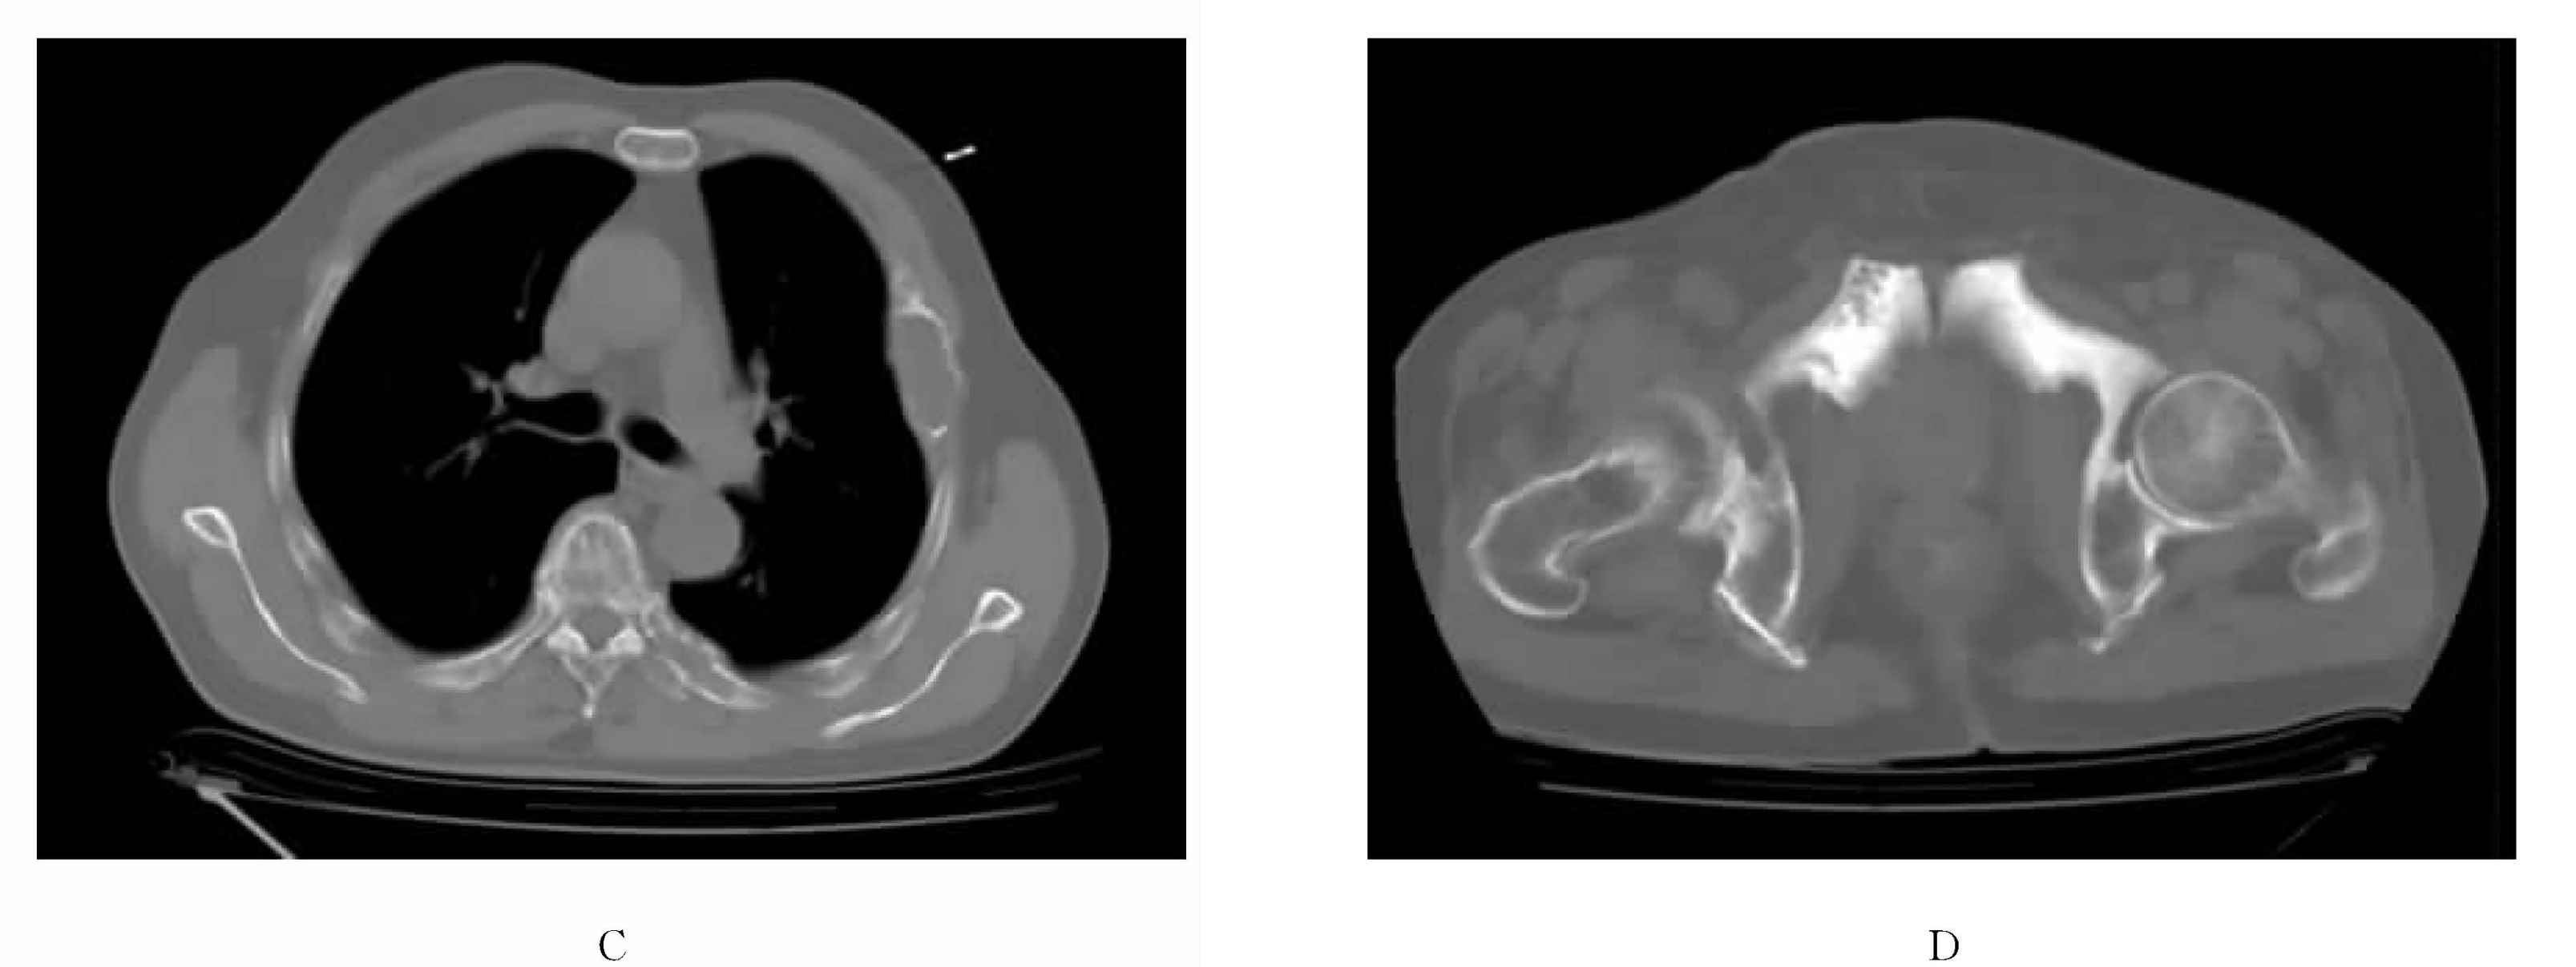
\includegraphics[width=.7\textwidth,height=\textheight,keepaspectratio]{./images/Image00447.jpg}
 \captionsetup{justification=centering}
 \caption{骨转移瘤\\{\small A、B为胃癌患者,右侧髂骨翼呈溶骨性骨质破坏,并可见巨大软组织肿块;C可见左侧多条肋骨有溶骨性骨质破坏,胸椎亦有骨质破坏;D膀胱癌患者,左右耻骨有片状不规则高密度灶,无软组织块}}
 \label{fig22-22}
  \end{figure} 

3.混合型:亦较少见,兼有上述两型的表现。

\subsection{小结}

原发性骨肿瘤可来源于骨组织、软骨组织、纤维组织、骨髓组织、脉管组织、神经组织、脂肪组织、间叶组织、脊索组织,还有一些来源不明。瘤样病变包括骨纤维异常增殖症、畸形性骨炎、骨囊肿、动脉瘤样骨囊肿、上皮样骨囊肿、骨内软骨下骨囊肿、骨内腱鞘囊肿。上述病变几乎均可发生于长骨和部分短管骨。

\subsubsection{胸壁原发性骨肿瘤及肿瘤样病变的病理分类}

原发性远较转移性少见,占全身原发性骨肿瘤病的5%~10%,其中80%发生于肋骨,其次为胸骨、锁骨、肩胛骨。

1.胸骨:以恶性居多,常见的有多发性骨髓瘤、淋巴瘤、骨肉瘤和滑膜肉瘤等。

2.肋骨:①恶性肿瘤:在成人常见的有多发性骨髓瘤、骨肉瘤、软骨肉瘤,其他小圆形细胞肿瘤、纤维肉瘤等均罕见。在儿童则以尤文氏肉瘤常见。②良性肿瘤及肿瘤样病变:较常见的有软骨类肿瘤(包括软骨瘤、骨软骨瘤、软骨黏液样纤维瘤,后者相对少见)、骨纤维异常增殖症、韧带样纤维瘤、血管瘤、巨细胞瘤及嗜酸性肉芽肿(年龄多较小)、囊肿等。

\subsubsection{肋骨囊状膨胀性骨质病变}

1.骨纤维异常增殖症:一般病变范围较长,多超过8cm;密度较高呈磨玻璃状;无骨膜反应。

2.肋骨结核:好发于第4~7肋骨中段,继发者位于肋骨头部,伴有椎体、附件结核病灶。破坏区总残留一些骨质或死骨存在,病变周围有骨质增生和骨膜反应,且可伴有广泛胸膜增厚及胸壁脓肿。

3.软骨瘤:与其他软骨类肿瘤一样好发于肋骨前端。可形成软组织肿块突入肺内,其内有点、弧、环形钙化。

4.骨巨细胞瘤:好发于肋骨头干骺处。病灶膨胀显著,无硬化缘及骨膜反应。

5.转移瘤:病灶可多发性,呈溶骨性破坏,无骨质增生及骨膜反应,软组织肿块局限(成骨性转移可无软组织肿块)且易向胸腔内突入。与骨髓瘤可难以鉴别,后者呈多发小圆形骨破坏,边缘清晰,软组织改变相对轻微。

\subsubsection{脊柱原发性骨肿瘤及肿瘤样病变的病理分类}

1.良性肿瘤及肿瘤样病变:主要有骨母细胞瘤、骨样骨瘤、血管瘤、骨软骨瘤、巨细胞瘤、动脉瘤样骨囊肿、嗜酸性肉芽肿、软骨黏液样纤维瘤、神经源性肿瘤。此外,畸形性骨炎易发生于脊柱(但骨盆和四肢多见,颅骨、股骨、胫骨易受累)。其中,骨母细胞瘤和骨样骨瘤以椎弓附件多见;巨细胞瘤和动脉瘤样骨囊肿主要涉及椎体,偶以附件为主,两者可难以鉴别。椎体血管瘤表现为局限性低密度区内的正常骨结构消失,代之以粗大稀疏的致密点,代表粗大稀疏的骨小梁;应注意与重度骨质疏松相鉴别,后者涉及椎体多、范围广泛、皮质变薄等有助于鉴别。

2.恶性肿瘤:主要有骨髓瘤、脊索瘤、骨肉瘤、软骨肉瘤、淋巴瘤,儿童还有尤文氏瘤。但是脊柱的恶性肿瘤以转移性多见,在诊断时应予注意。转移瘤好发于椎体中后部,且易累及椎弓根为其分布特点。

\subsubsection{骨盆原发性骨肿瘤及肿瘤样病变的病理分类}

1.良性肿瘤及肿瘤样病变:巨细胞瘤、动脉瘤样骨囊肿好发于骶骨,亦可发生于髋骨;骶骨神经源性肿瘤亦并非少见。此外,嗜酸性肉芽肿可发生于骶骨及髋骨,软骨母细胞瘤好发于髂骨体;骨盆软骨黏液样纤维瘤、韧带样纤维瘤、骨样骨瘤以及髂骨的骨纤维异常增殖症等亦时有报道。

2.恶性肿瘤:骶骨是脊索瘤的好发部位,骨髓瘤、骨肉瘤、软骨肉瘤、纤维肉瘤、淋巴瘤、恶性纤维组织细胞瘤、尤文氏肉瘤(见于儿童)均可发生于骨盆诸骨。但均不及转移瘤常见,应注意鉴别。

\subsubsection{颅骨原发性骨肿瘤和肿瘤样病变的病理分类}

1.良性肿瘤和肿瘤样病变:常见的有骨瘤、血管瘤、胆脂瘤、骨纤维异常增殖症、嗜酸性肉芽肿等。此外,骨软骨瘤、内生软骨瘤、巨细胞瘤、骨化性纤维瘤、骨囊肿、神经纤维瘤病等也时有发生。

但有时蛛网膜颗粒压迹可完全穿通颅骨骨板呈骨质缺损表现,甚至呈溶骨性破坏样表现。尤其在枕部,CT可表现为距窦汇3.0cm以内的、枕骨内板凹陷状压迹或穿凿状骨质缺损,最大可达3cm,应注意与骨肿瘤相鉴别(图\ref{fig22-23})。

\begin{figure}[!htbp]
 \centering
 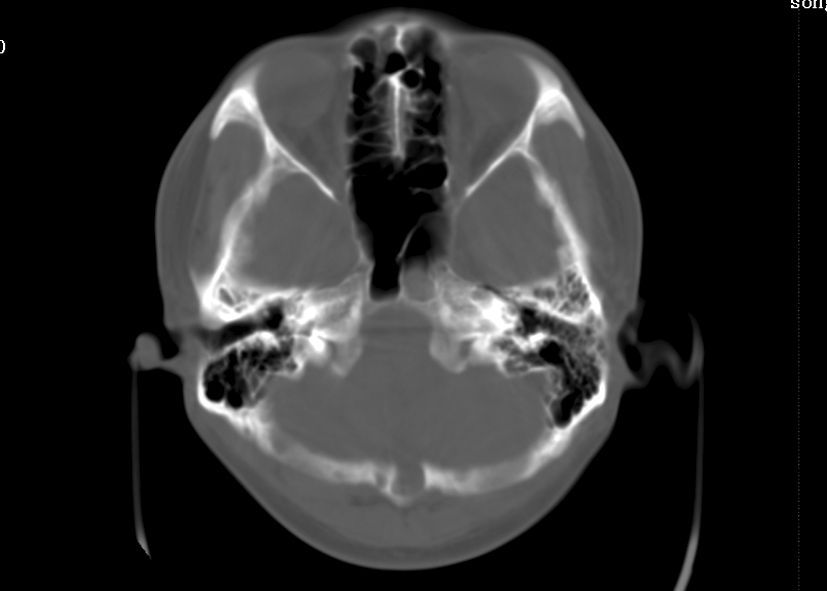
\includegraphics[width=.7\textwidth,height=\textheight,keepaspectratio]{./images/Image00448.jpg}
 \captionsetup{justification=centering}
 \caption{枕骨蛛网膜颗粒压迹\\{\small 枕骨可见颅骨内板、板障近囊状骨质缺损}}
 \label{fig22-23}
  \end{figure} 

2.恶性肿瘤:常见的有骨髓瘤、颅底脊索瘤。此外,软骨肉瘤、淋巴瘤等亦时有报道。

\subsubsection{动脉瘤样骨囊肿与巨细胞瘤的鉴别}

部分动脉瘤样骨囊肿无论是在临床、影像学还是病理上很难与巨细胞瘤完全区别开。有学者甚至认为动脉瘤样骨囊肿必然是由外伤或其他骨病所致,如果不能确定有前期病变,则考虑为巨细胞瘤。

鉴别诊断应注意的几点:①动脉瘤样骨囊肿好发于10~20岁;而巨细胞瘤好发于20~40岁。②前者长径与骨干平行;而后者与骨干垂直。③前者囊变进展快,加上容易骨折,可见骨膜反应,稳定期囊间隔可有钙化;而后者则无骨膜反应和钙化。④增强扫描后者远高于前者,而且前者35%出现液-液平面。巨细胞瘤出血后血细胞与血浆分离也可产生液-液平面,但少见。还有学者认为影像学表现不典型者,应考虑到二者并存可能。

此外,软骨母细胞瘤、骨肉瘤、骨囊肿、骨纤维异常增殖症等均可见液-液平面,应注意鉴别。

\section{软组织病变}

\subsection{脂肪瘤}

本病为较常见的软组织肿瘤,任何含有脂肪组织的部位都可发生。

\textbf{【病理】}
多见于颈、肩、背、臀及肢体的皮下组织和腹膜后,也可见于肠系膜、肾周和筋膜下。瘤周有薄层纤维包膜,呈扁平或分叶状,质软。镜下由成熟的脂肪细胞构成,其间有不规则纤维组织分隔。脂肪瘤瘤内可含有其他的间叶成分,如纤维结缔组织、黏液、软骨和平滑肌组织等,分别称为纤维脂肪瘤、黏液脂肪瘤、软骨脂肪瘤和肌肉脂肪瘤。

此外,脂肪瘤还有许多变异类型,与脂肪瘤的临床和组织学表现明显不同,如血管脂肪瘤(血管瘤成分中有成熟的脂肪细胞)、成脂肪细胞瘤、梭形脂肪细胞瘤、多形性脂肪瘤等。

\textbf{【临床表现】}
好发于50~70岁,多见于肥胖人群。典型表现为生长缓慢的无痛性肿块。皮色正常,基底宽,触之柔软。

\textbf{【CT表现】}
呈均匀一致的、边缘清楚锐利的低密度灶,CT值-120~-80Hu,与皮下脂肪CT值相近(图\ref{fig22-24})。有时可见不规则钙化。在肌间脂肪瘤中可见到条索状肌间隔。增强扫描无强化。

\begin{figure}[!htbp]
 \centering
 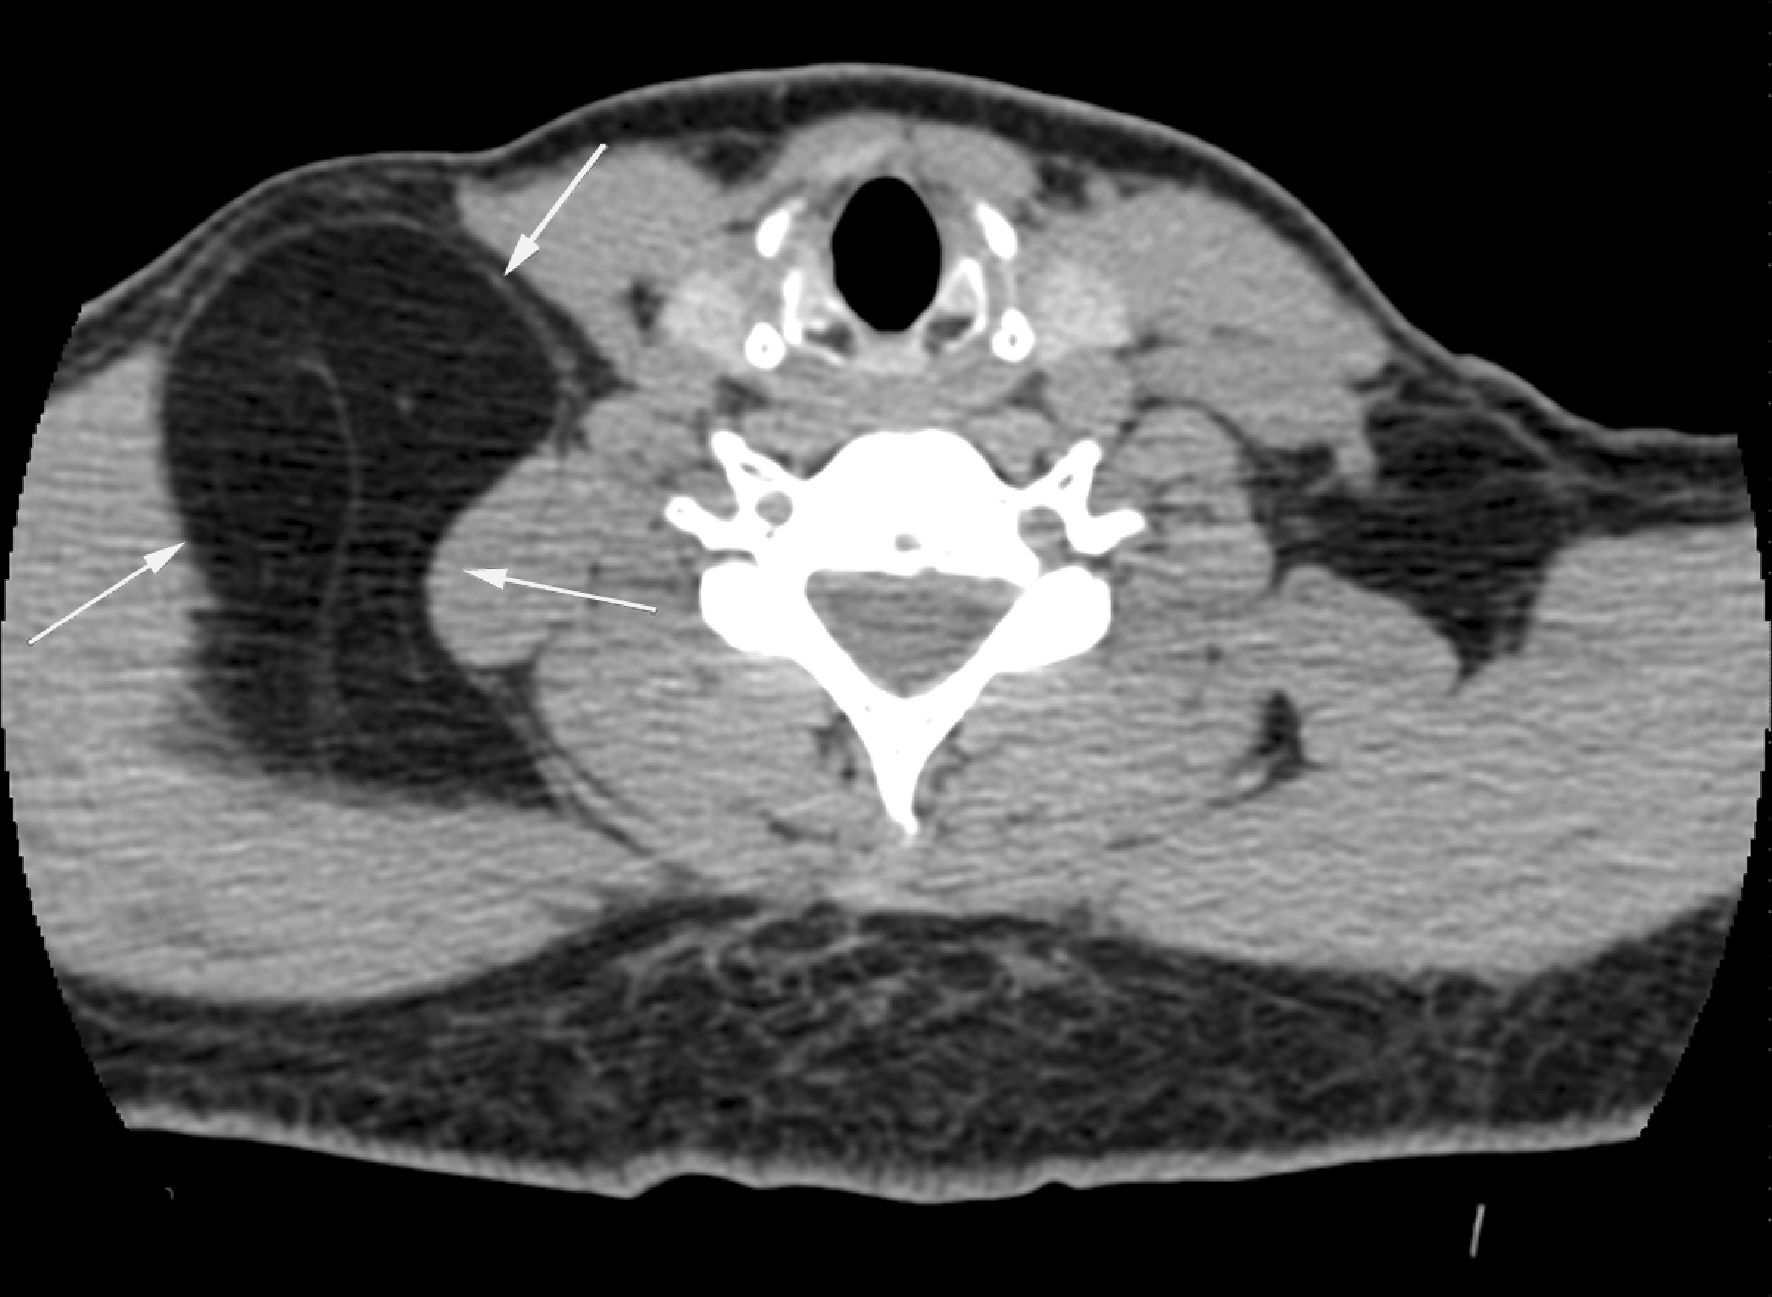
\includegraphics[width=.7\textwidth,height=\textheight,keepaspectratio]{./images/Image00449.jpg}
 \captionsetup{justification=centering}
 \caption{脂肪瘤\\{\small 右侧颈部可见近圆形脂肪密度灶}}
 \label{fig22-24}
  \end{figure} 

此外,所谓浸润性脂肪瘤也是一种良性肿瘤,但呈浸润性生长,术后易复发。CT示边缘不规则,可明显强化。

\subsection{血管瘤}

\textbf{【病理】}
血管瘤为血管组织形成的良性肿瘤,可发生于任何组织。发生于软组织者多见于皮肤、肌肉、滑膜和结缔组织中。组织学可分为海绵状血管瘤、毛细血管瘤。此外,还有静脉性血管瘤、上皮样血管瘤和肉芽肿样血管瘤。但以毛细血管瘤最多见,海绵状血管瘤次之,其他少见。

\textbf{【临床表现】}
多见于婴儿和儿童,女性为男性的2~3倍。多无明显症状,可有间歇性疼痛、肿胀。持续发展可侵犯、破坏周围组织。

\textbf{【CT表现】}
呈边界较清晰或不清晰的不均质软组织肿块,病灶中常见环状钙化的静脉石为诊断的重要依据;增强扫描显著强化,有时可见囊状不规则扩张的血窦或粗细不均、迂曲扩张的供血动脉及引流静脉。邻近骨骼者可有骨侵蚀、破坏表现。

\subsection{淋巴管瘤}

\textbf{【病理】}
好发于颈部、腋窝、口腔等部位,属先天性淋巴管发育畸形,而非真性肿瘤。其病理改变是淋巴管扩张、增生和结构紊乱。由许多小管、小囊或大囊形成多层性囊状结构,内含淡黄色液体。淋巴管瘤可分为毛细淋巴管瘤、海绵状淋巴管瘤和囊样水瘤。骨、软组织和内脏器官出现弥漫性或多发性淋巴管瘤时称为淋巴管瘤病。

\textbf{【临床表现】}
多见于儿童,在出生时即可存在,也可在出生后任何时期出现。发生于表浅部位者,呈水泡状或丘状隆起。发生于深部软组织者,呈柔软、无痛性肿块。肿瘤大者可出现邻近器官的压迫症状。

\textbf{【CT表现】}
呈囊性病变,多囊或单囊,以多囊多见;囊内可有分隔;易沿组织间隙生长是其特点。在颈部可广泛波及颈深部至皮下。呈均匀水样密度;囊内易有出血而使平扫密度增高或出现囊内液-液平面。囊壁罕有钙化,可轻度强化。囊样水瘤可自行消退,但病变部位越深、越复杂,复发可能性越大,抽吸还可能导致液体的迅速重新积聚。

\subsection{血管球瘤}

本病又称血管神经瘤、血管肌肉神经瘤等。起源于动脉-静脉间的血管球,多发生于皮肤和皮下组织,可引起骨骼的受压受侵。

\textbf{【病理】}
正常血管球体是一个微小的球形终末器官,由输入动脉、吻合的血管、原发的侧支静脉、血管球间网、包囊等部分组成。婴儿没有血管球体,60岁以上也减少。血管球体收缩机能可控制皮肤动静脉循环的作用,因而能调节血流和体温。病理上血管球瘤体积较小,界限清楚;由多少不等的小血管构成。

\textbf{【临床表现】}
本病罕见,以成人多见,男女发病率相近。主要累及软组织,好发于末节指骨和甲下,也可见于足底、耳廓、鼻及臀部等处。指端者表现为皮下或甲下的浅蓝或紫红色小结节,直径一般在数毫米至1cm。有明显的疼痛和触痛,对冷热敏感;轻微的机械或冷热刺激即可出现针刺样剧痛。

\textbf{【CT表现】}
指(趾)端者可见局部软组织密度结节,肿瘤压迫侵蚀邻近骨质可见边缘不规整或局限性骨质吸收破坏,甚至呈囊状破坏,无钙化和残留骨。增强扫描可显著强化。

\textbf{【鉴别诊断】}
发生于指端的血管球瘤平片与表皮样囊肿(一般为外伤性植入性)鉴别困难,需注意密切结合病史和临床表现相鉴别,但增强扫描后者无强化。此外,还应注意与腱鞘巨细胞瘤相鉴别,后者因有含铁血黄素沉积,MRT\textsubscript{2}
WI表现为中等至低信号是其特点。

\subsection{神经源性肿瘤}

神经源性肿瘤可分为神经鞘瘤和神经纤维瘤。前者起源于神经鞘细胞(雪旺细胞),后者起源于神经内膜的神经母细胞。

\textbf{【病理】}

1.神经鞘瘤:大多由梭形细胞组成,通常完整的有包膜,常有坏死、囊变等。病理主要由Antoni
A区和Antoni B区组成。Antoni A区细胞排列紧密,Antoni
B区细胞少,排列稀疏呈网格状;细胞间有黏液变性和高脂质。各种神经鞘瘤两者的比例不同,可以从完全的Antoni
A区,逐渐过渡到两者交错,甚至完全被Antoni
B区所占据,更有甚者可完全退变形成一个大囊。

2.神经纤维瘤:含有全部神经纤维组织成分,也可包含雪旺细胞或富脂质细胞,肿瘤间质由含量不等的纤维黏液样基质构成,无包膜。神经常穿越在肿瘤之中而不受推移。常为实性,因肿瘤内含有各种成分,故亦可有坏死、囊变,但少见。

\textbf{【临床表现】}
多发生于20~50岁成人。一般病程较长,除颈部肿块外,多无其他症状。肿块边缘清,表面光滑,呈囊性或较软的多为神经鞘瘤。

神经鞘瘤可发生于身体各部,如颈部、胸膜、腋窝、腹壁、盆腔和臀大肌等处,其中以皮下组织多见,其次为肌肉组织。临床症状轻微,多在体检时偶然发现。

神经纤维瘤常发生于皮肤神经,极少累及较大的神经而发生于深部组织。90%左右单发,肿块较大时临床症状明显,否则可无明显症状。如肿块出现疼痛或增大,尤其存在多发病灶(神经纤维瘤病),应注意是否有恶变可能。

\textbf{【CT表现】}

1.神经鞘瘤:肿瘤呈边缘光滑的圆形、卵圆形或梭形肿块,因具有包膜,肿块与毗邻组织分界清楚。肿块密度与肌肉组织相近,可有坏死液化区,甚至偶可钙化。增强扫描包膜及实性部分有轻中度强化。

2.神经纤维瘤:肿瘤表现为界限清楚、密度均匀的软组织肿块,呈梭形,沿神经方向走行,位于肌间隙内。增强扫描可见强化。

\subsection{侵袭性纤维瘤病}

本病又称韧带样纤维瘤病,是一种很罕见的疾病。纤维瘤病又称瘤样纤维组织增生,是一组良性纤维组织增生的病变(有文献认为形成瘤样肿块,但非真性肿瘤),包括韧带样纤维瘤病、瘢痕疙瘩、结节性筋膜炎等,与良性纤维瘤的区别是无包膜、有侵袭性等。

\textbf{【病因病理】}
其发生与外伤、手术、激素水平有关。本病根据发病部位分为:①表浅或筋膜纤维瘤病:包括手掌、足跖纤维瘤病,阴茎纤维瘤病和婴儿指、跖纤维瘤病。②深部纤维瘤病:包括腹壁纤维瘤病、腹壁外纤维瘤病、腹腔和肠系膜纤维瘤病和婴儿纤维瘤病。

组织学上由成束分化好的成纤维细胞、成肌纤维细胞及多少不等的胶原构成,形成无包膜、轮廓不清的肿物,有时成纤维细胞生长活跃,甚至有一定的异型性,有时可有假包膜。本病虽属良性,但呈浸润性生长,且易复发,即其生物学行为介于良性纤维瘤与纤维肉瘤之间。

\textbf{【临床表现】}
好发于25~45岁成人(70%),少数发生于婴儿及儿童。男女之比为1∶2。多表现为体积较大的浸润性肿块,术后常复发。激素和放疗对肿瘤治疗有效。

\textbf{【CT表现】}

1.腹部侵袭性纤维瘤病:可发生于腹壁(50%)、肠系膜(41%)和腹膜后(10%),以侵犯腹直肌最多。本病腹部者可属于Gardner综合征的一部分。

CT显示肿瘤截面为梭形或卵圆形,沿腹直肌和(或)腹斜肌等长轴生长,边缘规则。密度基本均匀,平扫或增强扫描与肌肉密度相近。腹膜后者应注意与特发性腹膜后纤维化相鉴别。

2.腹壁外侵袭性纤维瘤病:多位于四肢、躯干深部软组织,以肩部最常见。以下依次为胸背部、大腿、颈、膈等。

CT显示肿瘤沿肌肉长轴生长,边缘不规则,范围广泛。肿瘤明显侵犯周围肌肉、骨骼等结构。肿瘤强化可略高于肌肉或密度欠均。

\subsection{腱鞘巨细胞瘤}

本病又称良性滑膜瘤、骨膜纤维黄色瘤、局限性结节性滑膜炎、巨细胞性腱鞘炎等。因其病理改变与色素绒毛结节性滑膜炎相同,多认为两者属同一疾病,并将其归为后者的腱鞘型。

\textbf{【病理】}
肿瘤来源于滑膜细胞,多呈结节状、分叶状肿块。肿瘤由不同比例的单核细胞、多核巨细胞、泡沫细胞(载脂细胞)、含铁血黄素细胞和慢性炎性细胞构成。肿瘤间质内含有胶原纤维,常有不同程度的玻璃样变性及含铁血黄素沉积。

\textbf{【临床表现】}
好发于20~40岁,男女之比约为1∶2。主要发生于手指的指端及指间关节处,其次为足趾、膝关节、足踝部、手腕甚至髋关节附近。多数呈无痛性结节,生长缓慢。

\textbf{【CT表现】}
多呈局限性密度增高的软组织结节,界限清晰,大小多不超过2~3cm。邻近骨质压迫性吸收破坏,或呈边缘清楚的囊状破坏。6%病灶内有钙化。

\subsection{肌肉内黏液瘤}

本病是一种深部肌肉的良性肿瘤。

\textbf{【病理】}
肌肉内条形肿块,质地硬、边缘清楚,肿瘤外常有薄层假膜。镜下肿瘤由均质性、含细胞结构少的黏液构成,细胞浸泡在黏液中。合并骨纤维异常增殖症时称为Mazabraud综合征。

\textbf{【临床表现】}
多见于40岁以上,男女发病相近。发病部位一般在肢体较大肌肉,常见部位为大腿、臀部和上臂。表现为局部生长缓慢的、无痛性肿块。

\textbf{【CT表现】}
病灶呈圆形或卵圆形软组织肿块,典型者密度低于周围肌肉,CT值多为10~30Hu,密度均匀,界限清晰。增强扫描无强化。

主要应与神经鞘瘤相鉴别,本病增强扫描无强化,而神经鞘瘤实性部分多有强化。

\subsection{脂肪肉瘤}

脂肪肉瘤是常见的软组织恶性肿瘤。通常认为是原发的,而不是由良性脂肪瘤恶变而来。

\textbf{【病理】}
通常体积较大,直径多在5~15mm。一般无包膜,可向周围组织浸润。瘤体组织因病理类型不同而呈灰黄色、胶冻样、脑髓样、鱼肉样。组织学上,脂肪肉瘤由脂肪细胞和各种软组织成分混合而成,因此其密度差异较大。肿瘤内可见出血、坏死或囊变,10%含有钙化。可分为4型,即脂肪瘤样型、黏液样型、圆细胞型和多形型。

\textbf{【临床表现】}
多见于中老年人,儿童极为少见,男女之比约4∶1。临床表现为深部无痛性肿块,边界不清,或部分固定于软组织内。晚期可有疼痛或功能障碍。

\textbf{【CT表现】}
呈边界不清、密度不均匀的肿块。病灶中可见脂肪密度和水样密度区域,如CT值<20Hu,一般认为是脂肪成分而不是坏死组织。分化不良的脂肪肉瘤呈软组织密度肿块,瘤内较少或无脂肪成分(图\ref{fig22-25})。增强扫描呈不均匀强化。

\begin{figure}[!htbp]
 \centering
 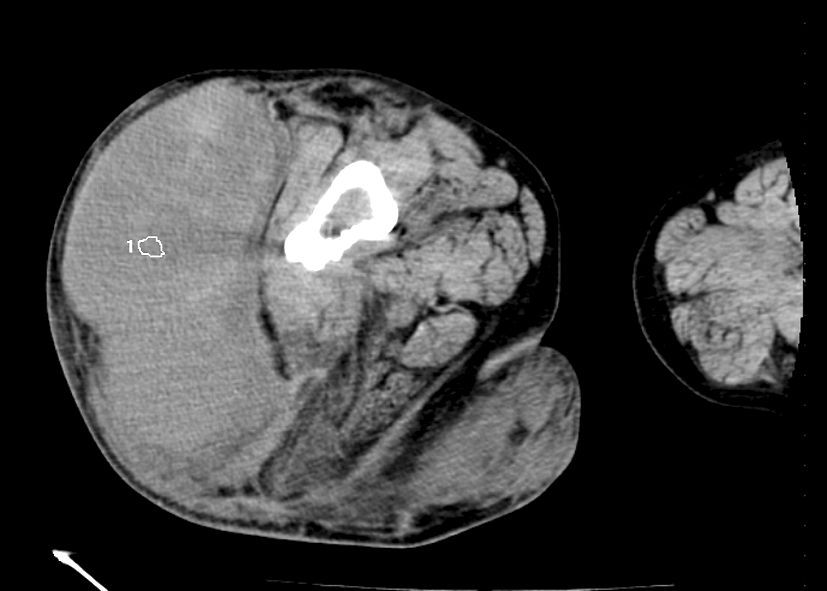
\includegraphics[width=.7\textwidth,height=\textheight,keepaspectratio]{./images/Image00450.jpg}
 \captionsetup{justification=centering}
 \caption{脂肪肉瘤\\{\small 右侧股部有巨大软组织肿块,密度欠均、CT值约24Hu,边缘欠清晰}}
 \label{fig22-25}
  \end{figure} 

\subsection{恶性纤维组织细胞瘤}

本病又称为纤维组织细胞肉瘤。

\textbf{【病理】}
四肢多见。多数学者认为起源于间叶细胞,可向纤维细胞和组织细胞分化,具有多种细胞成分。肿瘤呈结节状,多血管丰富,常有假包膜。瘤内可见出血或坏死灶,偶见钙化灶。显微镜下可见肿瘤细胞具有多形性,主要由成纤维细胞样细胞、异形巨细胞、泡沫样细胞等组成。组织学可分为5种病理类型:①纤维型:约占2/3;②巨细胞型;③黏液型;④炎症型;⑤黄色肉芽肿型。

\textbf{【临床表现】}
主要表现为软组织肿块和局部疼痛,病程长短不一。本病术后复发率高达45%,转移率为42%。

\textbf{【CT表现】}
呈界限不清的软组织肿块,密度略低,多无钙化。肿块内常有低密度坏死区。肿块可向周围侵犯邻近的血管、神经。增强扫描病灶强化不显著。

\subsection{横纹肌肉瘤}

本病约占全部软组织肉瘤的20%,是20岁以下软组织中最常见的肉瘤。

\textbf{【病理】}
可分为胚胎型、腺泡型和多形型。胚胎型大多以未分化细胞占优势,肿瘤以小圆形细胞为特征。腺泡型由未分化的小圆形、卵圆形细胞所组成,并聚集成为实质性小岛或小泡。多形型是一种具有球形细胞、梭形细胞、巨细胞和球拍状及蝌蚪样细胞的多形性肿瘤。

\textbf{【临床表现】}
胚胎型多见于6岁以下儿童,好发部位是头颅的腔道结构,以及头颅软组织内;腺泡型多见于青少年;多形型多见于老年人。后两型多见于四肢,尤其是下肢。肿瘤生长迅速,具有较大的侵袭性和破坏性。本病容易被早期发现;除邻近神经受压外,不引起疼痛。

\textbf{【CT表现】}
表现为不均匀的软组织肿块,界限较清晰,周围的骨质、血管、神经可被侵犯(图\ref{fig22-26})。但其表现无特异性,与其他恶性肿瘤无法鉴别。

\begin{figure}[!htbp]
 \centering
 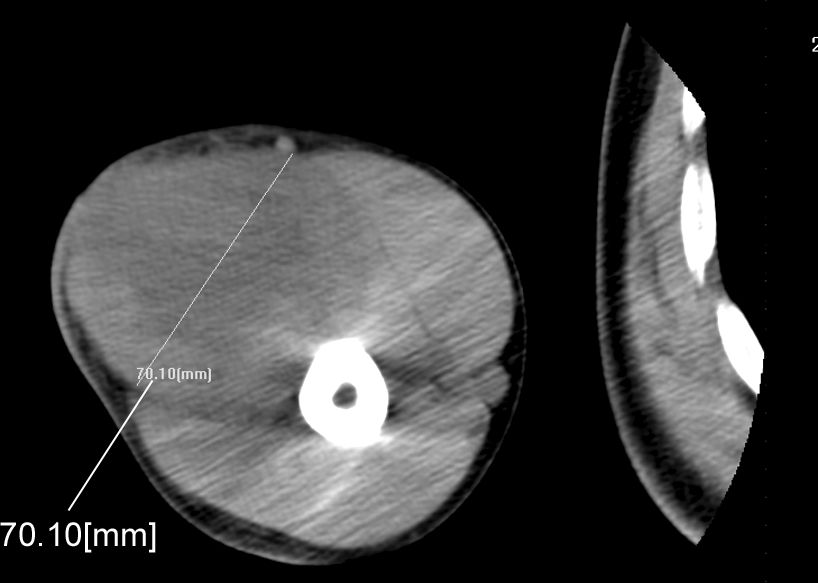
\includegraphics[width=.7\textwidth,height=\textheight,keepaspectratio]{./images/Image00451.jpg}
 \captionsetup{justification=centering}
 \caption{横纹肌肉瘤(多形型)\\{\small 39岁男性,右上臂有巨大软组织肿块,密度不均,边缘欠清晰}}
 \label{fig22-26}
  \end{figure} 

\subsection{纤维肉瘤}

本病是较为常见的软组织恶性肿瘤,也易波及骨组织。

\textbf{【病理】}
起源于成纤维细胞。可发生于身体的各个部位,但以大腿和膝部最常见,其次是躯干和四肢远端。肿瘤质地硬或软,常侵犯周围组织,也可有假包膜。较大者可有出血、坏死、囊变。软组织深部者可侵入骨内,甚至达髓腔。镜下主要由似成纤维细胞的瘤细胞及其间的多少不等的胶原纤维、网状纤维组成,但组织结构变异很大。瘤细胞的间质可有骨和软骨化生及黏液变性,但不多见。

\textbf{【临床表现】}
多见于30~55岁的中年人,女性略多见。主要表现为生长缓慢的孤立性硬实肿块,一般无疼痛。生长部位深浅不一。

\textbf{【CT表现】}
表现为圆形或分叶状软组织肿块,界限清晰或不清晰,密度不均匀,钙化少见。发生于四肢者,易向近侧沿血管、神经束扩展。但其表现无特异性,与其他恶性肿瘤无法鉴别。

\subsection{肌肉淋巴瘤}

本病罕见,包括原发性和继发性两种,多见于广泛播散期或复发病例。国外报道原发性好发于四肢,尤其是大腿及上肢;继发性以腰大肌和髂肌最常见。近期国内报道1组,仅1例为原发性;继发性的好发部位为髂腰肌、腰大肌和髂肌,多为多块肌肉同时受累。

\textbf{【病因病理】}
肌肉淋巴瘤的发病机制包括:①经血液或淋巴途径侵犯肌肉;②邻近病变直接侵犯肌肉:例如骨或淋巴结的原发淋巴瘤可侵犯肌肉,相对较常见;③原发性:十分少见。无论原发还是继发,NHL占大多数。国内报道1组NHL占82%,HD占18%。

\textbf{【临床表现】}
各年龄层均可发病,以中老年多见。主要表现为疼痛、肿胀或全身不适,部分可无自觉症状。

\textbf{【CT表现】}
原发性与继发性表现相似。多表现为肌肉增大或肿物,可同时有多处相连或不相连的肌肉受侵,不同肌肉的受侵程度不同。若位置表浅,局部皮肤可增厚,皮下脂肪内可见条索、网状改变。平扫病灶密度略低或等于正常肌肉,增强扫描可等于、轻度高于或明显高于正常肌肉。病灶内常可见坏死或变性所致的低密度区。

此外,原发性骨淋巴瘤常伴软组织肿块。国外有学者认为伴有软组织肿块的骨淋巴瘤,即使CT没有骨皮质破坏,亦不能排除病变侵犯周围软组织的可能。

\subsection{软组织钙化与骨化}

1.钙化与骨化:所谓软组织钙化是指软组织内有钙盐沉着,呈均质性或斑点状高密度灶,其内不显示任何结构;而骨化则指浓密阴影内可显示骨结构者。但二者并无截然界限,钙化可移行至骨化,且钙化往往是骨化的开始。软组织钙化除生理性钙化外,可因创伤、感染(寄生虫、细菌)、肿瘤、代谢性疾病、血管性疾病等所引起,而且常与局部酸碱度的变化有关。

2.转移性钙化:为钙磷代谢障碍,钙盐自骨组织移入软组织内的结果。常见于各种引起高血钙的疾病,如甲状旁腺功能亢进、特发性高血钙、维生素D增多症和慢性肾功能衰竭等。

3.营养不良性钙化:为组织本身的退行性变、纤维化和坏死形成,体液中钙磷的含量正常。如血管壁钙化、血肿钙化、静脉淤滞所导致的皮下组织钙化和骨化、关节周围钙化、寄生虫钙化(囊虫病、丝虫病、旋毛绦虫病)等。

\subsection{局限性骨化性肌炎}

本病可分为外伤性和非外伤性,其中外伤性约占60%~75%。

\textbf{【病因病理】}
本病是因肌肉变性、出血或坏死所致。常于外伤后3~4周出现钙化和骨化,骨化自外周向中央发展。病灶呈圆形或卵圆形,最大径多为3~7cm,可达10cm。镜下具有特征性的分带现象:中央带为不成熟、富血管、增生活跃的纤维组织;中间带为类骨组织,形成不规则相互吻合的小梁,间杂有成纤维细胞和骨母细胞;外带为成熟的骨组织。最后整个病灶可以骨化。

\textbf{【临床表现】}
好发于青年男性。多位于易受外伤处,如股四头肌、骨内收肌及上臂肌肉内等。但不限于肌肉,还可见于肌腱、筋膜、骨外膜,甚至皮下脂肪组织内。外伤后早期局部明显肿胀、疼痛,可扪及软性肿块,邻近关节活动受限;后期(伤后10周至6个月)肿块逐渐缩小、变硬,症状减轻或消失,只遗留硬实性肿块。

\textbf{【CT表现】}
外伤后软组织内出现局限性肿块;3~4周肿块区出现毛糙不齐的密度增高区即钙化区,此后出现条状或层状骨化影,邻近骨骼可发生骨膜反应。

典型表现为环状钙化或骨化,边缘致密而中间较淡,呈卵壳状、囊肿样改变;数日后呈大片骨质影,肿块可部分或完全钙化或骨化。骨化多发生于邻近长骨的骨干部分,很少延及骨端及关节。

\textbf{【鉴别诊断】}
骨化性肌炎骨化后有骨小梁结构,无包绕骨干的生长趋势,且局部无浸润性软组织肿块。尤其后者与皮质旁骨肉瘤鉴别意义较大。

\subsection{进行性骨化性肌炎}

本病又称进行性骨化性纤维结构不良,是一种少见的先天性遗传性疾病。

\textbf{【病因病理】}
病因不明,可能为中胚层发生或发育异常。以韧带、腱膜和横纹肌发生进行性骨化为特征。病变开始于筋膜、肌腱及肌肉间纤维间隔结缔组织,而不是肌肉纤维本身,之后才相继侵犯肌肉。早期为肌肉和皮下组织的结节状肿胀(水肿及成纤维细胞增生);后期有胶原纤维增生,形成纤维性结节,随后发生钙盐沉着及骨化。

\textbf{【临床表现】}
多见于10岁以下儿童,10%有家族史,通常幼儿时期即发病。早期可有局部肿、痛、热,数天后消退遗留下发硬区;数周后发生骨化,引起收缩畸形。病变呈进行性,进展缓慢,缓解与进展交替出现,可造成患者终身残废以至死亡。常伴有先天性指(趾)畸形,如短小、缺如等。

\textbf{【影像学表现】}
病变多从颈背部开始,然后延及躯干和四肢,而且躯干和四肢常对称发病。早期表现为软组织肿胀,之后出现不规则点条状钙化,最后形成斑片状或带状致密影。钙化或骨化沿肌束、肌腱或韧带方向走行,断面上钙化由中央部开始逐渐向外扩展。骨化的肌肉呈扁平或条状,并与骨骼相连。脊柱韧带亦可广泛骨化,甚至呈竹节状。

\subsection{钙化性关节周围炎}

\textbf{【病因病理】}
本病多数为损伤和退行性变所致。钙质沉着于关节周围的肌腱、腱鞘、筋膜、关节囊或滑囊。常见于肩、膝、髋、肘、腕和手部关节附近,尤以肩部常见。

\textbf{【临床表现】} 表现为关节疼痛和活动受限。

\textbf{【影像学表现】}
钙化形态可呈斑点状、斑片状或条状。肩部钙化好发于冈上肌腱靠近它附着于肱骨大结节处。髋部钙化多见于股骨颈的上方、关节间隙外侧。膝关节周围的钙化或骨化多位于内收肌结节、内收肌腱及内侧副韧带外方的一层腱膜上。

此外,肘、腕、手以及髋部的钙化可在数周或数月后全部或部分吸收,部分则永久保留。

\subsection{特发性钙质沉着症}

本病为一种原因不明的独立疾病。其特征为皮肤、皮下组织、浅层肌肉、肌腱的钙质沉积。

\textbf{【病因病理】}
其病因不明,本病常与其他疾病如硬皮病、皮肌炎、甲旁亢等并存;也可能与维生素D应用过量、慢性肾病、骨折长期卧床、外伤、炎症、长期服用碱性药物等有关。病理主要改变为脂肪组织及结缔组织变性,并有不规则钙质沉着,钙化肿块有纤维包膜和分隔。根据病变的范围和形态可分为3型。①局限型:少数部位皮下发生钙化,常累及指(趾)骨末端及关节;②弥漫型:全身多处部位发生钙化,以女性多见,多见于小儿及青年;③肿瘤型:大关节周围分叶状钙化(该型目前认为属常染色体显性遗传,为先天钙磷代谢异常所致,多见于青壮年女性)。

\textbf{【临床表现】}
症状不一。邻近关节的病变常引起疼痛及肢体活动障碍,如钙化部位表浅可以触及。如病灶穿破皮肤流出粉笔末样物为本病较特征的表现。

\textbf{【影像学表现】}
呈大小不一的钙化影。四肢钙化可单侧发生,亦可双侧发分布,钙化呈细条状、砂粒状、团块状等。有的钙化沿血管周围发生,呈腊肠状或龙蟠柱状。①局限型:常见指(趾)末端及邻近软组织内,以掌侧多见。②弥漫型:病变呈进行性。钙化首先见于皮下,其后渐渐延及皮肤、肌腱和肌肉等,最后出现于关节周围的皮下组织。病变虽广泛分布,但常出现于四肢易受伤部位,并沿肢体长轴分布。③肿瘤型:常为较多的钙化结节聚在一起,形态不规则。有时呈多囊状肿块,囊壁有薄层钙化或高密度线样结构,囊腔中心呈低密度。

\textbf{【鉴别诊断】}
骨化性肌炎多继发于外伤后,呈点片状骨化影,与钙质沉着症的结节状钙化迥然不同。

\subsection{滑液囊肿}

滑液囊肿在关节周围经常见到,以膝关节最多见。

\textbf{【病因病理】}
滑液囊肿与关节创伤性退变、炎症有关,可伴关节积液。是滑膜通过关节囊的疝出,囊肿内通常含有液体。

\textbf{【临床表现】}
可发生于各个年龄组。囊肿大者可出现酸胀、不适、疼痛,并可出现关节疼痛及活动受限。

\textbf{【CT表现】}
囊肿位于关节边缘,呈圆形、椭圆形或分叶状,边缘清楚、密度均匀的水样密度病灶,增强扫描无强化(图\ref{fig22-27})。

\begin{figure}[!htbp]
 \centering
 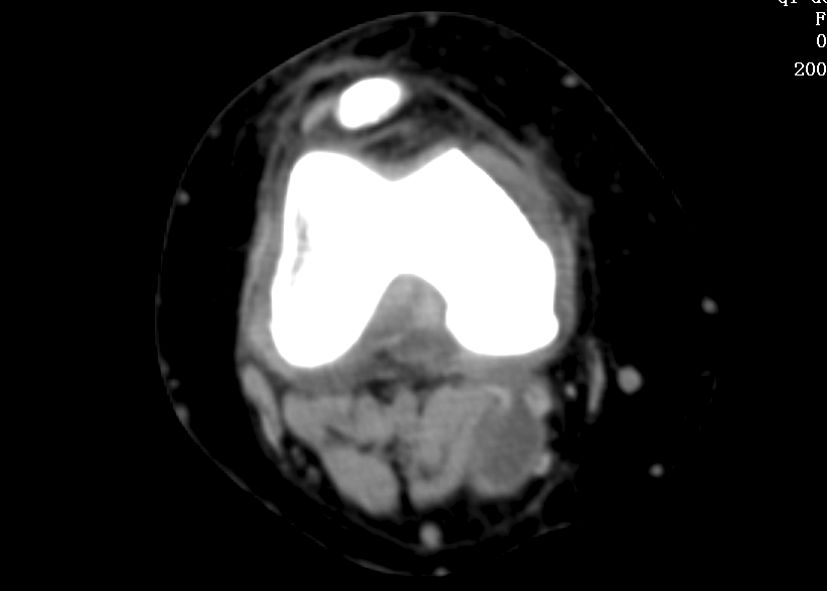
\includegraphics[width=.7\textwidth,height=\textheight,keepaspectratio]{./images/Image00452.jpg}
 \captionsetup{justification=centering}
 \caption{腘窝囊肿\\{\small 右侧腘窝区可见近水样密度灶,向前与关节腔相通连}}
 \label{fig22-27}
  \end{figure} 

\subsection{软组织血肿}

软组织血肿常发生于外伤后,亦可见于凝血功能障碍如血友病患者。

\textbf{【CT表现】}
新鲜血肿呈高密度灶,随时间推移而逐渐降低,或血肿密度高低不均。反复多次出血者,平扫可见血肿呈分层状高低不均(图\ref{fig22-28})。1个月后血肿区变为边界清楚、均匀一致的低密度区。增强扫描血肿壁显著强化。

但应注意结合临床与软组织脓肿相鉴别(图\ref{fig22-29})。

\begin{figure}[!htbp]
 \centering
 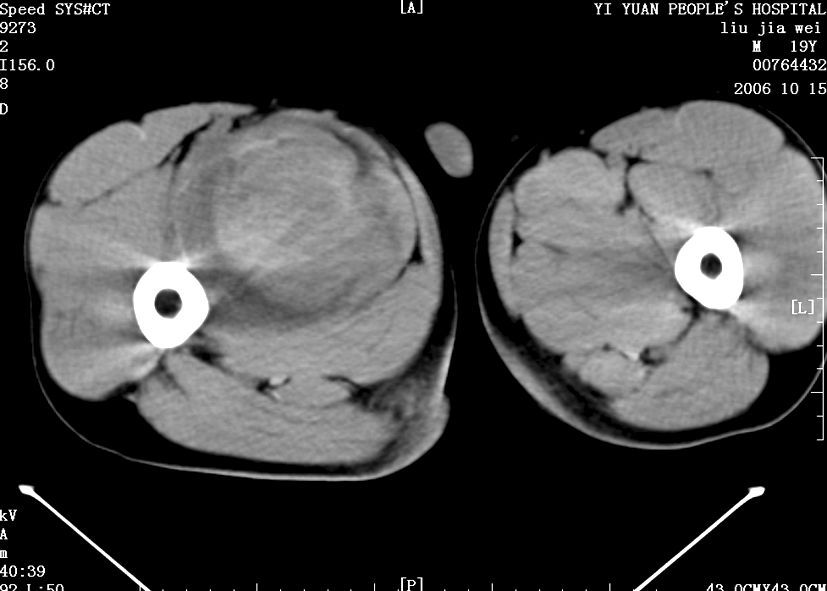
\includegraphics[width=.7\textwidth,height=\textheight,keepaspectratio]{./images/Image00453.jpg}
 \captionsetup{justification=centering}
 \caption{软组织血肿\\{\small 右侧股部内侧可见巨大分层状等低密度灶,边缘清晰}}
 \label{fig22-28}
  \end{figure} 

\begin{figure}[!htbp]
 \centering
 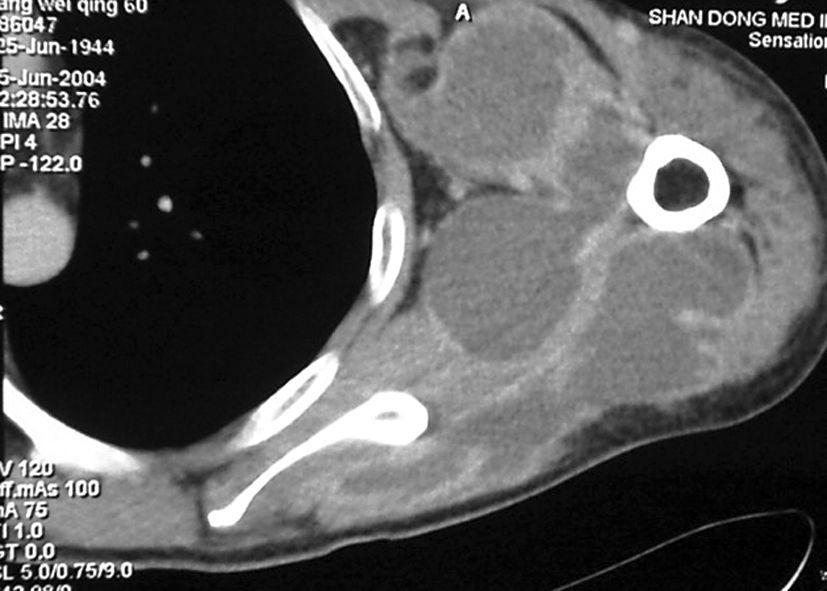
\includegraphics[width=.7\textwidth,height=\textheight,keepaspectratio]{./images/Image00454.jpg}
 \captionsetup{justification=centering}
 \caption{软组织脓肿\\{\small 左肩关节周围有多个囊状和不规则状近水样密度区,边缘清晰}}
 \label{fig22-29}
  \end{figure} 

\section{关节疾病}

\subsection{类风湿性关节炎}

类风湿性关节炎(RA)是以多发性、非特异性慢性关节炎症为主要表现的全身性疾病,以对称性侵犯手足小关节为特征。

\textbf{【病因病理】}
病因不明。多认为本病是免疫系统调节功能紊乱所致的免疫性疾患,多是在遗传易患素质的基础上、加上环境因素而致病。遗传因素可能与人类白细胞抗原-DR\textsubscript{4}
(HLA-DR\textsubscript{4}
)有关;环境因素主要为病毒或细菌感染,以及寒冷、潮湿、疲劳、创伤及精神刺激等。主要病理变化为关节滑膜的非特异性慢性炎症。初期以渗出为主,随后滑膜血管翳形成,并侵蚀软骨和骨等结构。晚期关节面粘连、关节腔消失,软骨表面肉芽组织纤维化骨化,使关节融合强直。病人常有滑囊炎、肌腱炎和腱鞘炎。

\textbf{【临床表现】}
高发年龄为45~54岁,男女之比为1∶3。起病和发展均较缓慢,呈多关节、对称性、游走性发病,从四肢小关节开始。局部关节肿胀疼痛、活动受限、晨僵等。全身症状有低热、乏力、食欲下降等,血沉加快,10%出现皮下结节,90%类风湿因子阳性。晚期表现为多关节畸形。

\textbf{【影像学表现】}
①关节软组织肿胀;②关节间隙变窄和关节边缘侵蚀;③骨质内小囊状破坏;④骨质疏松;⑤关节畸形、脱位或骨性强直;⑥早期可见到骨膜反应,晚期可见到关节退行性变。

\subsection{强直性脊柱炎}

\textbf{【概述】}
强直性脊柱炎(AS)是一种原因不明的慢性非特异性炎症。主要侵犯中轴骨、骶髂关节受累和附着病(即肌腱、韧带、关节囊和骨间膜等附着部位的炎性及增生性反应,可见于股骨大小粗隆、坐骨结节、坐骨棘、髂嵴、棘突、跟骨、胫骨结节、尺骨鹰嘴、胫腓骨间和尺桡骨间)为其特征。20世纪60年代以前被列为类风湿性关节炎的一个型别即中心型,1963年在美国类风湿病学会的分类中将类风湿性脊柱炎改为强直性脊柱炎。近年来的研究发现无论从临床表现、遗传因素、免疫反应、病理变化、影像学方面两者皆有明显不同,如临床检验AS类风湿因子(RF)为阴性,而人类白血球抗原(HLA-B\textsubscript{27}
)多为阳性,且HLA-B\textsubscript{27}
阳性者AS发病率可达10%~20%,而普通人群仅0.1%~0.2%。本病可伴发胸肋锁骨肥厚症(现多称为SAPHO综合征,即滑膜炎、痤疮、脓疱疮、骨肥厚、骨炎综合征),亦可伴发类风湿性关节炎,与某些肠炎亦具有相关性。

\textbf{【病因病理】}
AS可能与细菌、病毒感染、内分泌失调、受潮湿、受累、营养不良有关。其病理改变主要为附着病和滑膜炎。虽与类风湿性关节炎相似,但与类风湿性关节炎相比,渗出性变化、炎性细胞浸润较轻,而增生性变化是明显的,从而引起关节囊及其周围韧带的钙化骨化。

\textbf{【临床表现】}
多发生于30岁以下男性,男女之比为5∶1。本病具有家族性和遗传性。全身症状出现在关节改变之前,如周身无力、酸痛、体重下降、食欲不振,甚至贫血。进展期血沉增快、WBC可升高。本病早期诊断困难,多有腰背酸痛,尤以腰骶部显著。外周关节痛多位于下肢,尤以髋关节显著;跟骨和跟腱亦可疼痛,约1/4发生虹膜炎,还可有主动脉炎、心肌病、肺纤维化和肾损害等。临床检验RF为阴性、HLA-B\textsubscript{27}
90%呈阳性、C-反应蛋白可升高;免疫组织化学分析浆细胞浸润以IgG、IgA型为主(而RA则以IgM为主)。随着病情的进展,症状可有所减轻而强直加重,患者出现驼背、呼吸困难、脊柱强直。

\textbf{【影像学表现】}
本病几乎100%侵犯骶髂关节,而且多为其前驱病变。据报道,最初的影像学表现99%以上为骶髂关节炎,随后绝大多数逐渐上行性侵犯脊椎,最终累及颈椎。极少数可有跳跃性病灶,即骶髂关节与胸椎和(或)颈椎受累,而腰椎正常。关于AS可呈下行性发病的说法难以定论。髋关节是AS最易受累的周围关节,其病变可早于骶髂关节,一般年龄小者易累及髋关节。

1.典型表现

早期可见双侧骶髂关节对称性病变,仅11.4%的病例开始发生于一侧骶髂关节,而对侧在几个月或一年内相继发生。病变自骶髂关节的下2/3开始。因髂骨侧的软骨较骶骨侧薄,所以髂骨侧关节面的改变早且显著。①早期骶髂关节边缘呈锯齿状伴小囊状破坏,继而范围进一步广泛,并出现明显硬化,最后变窄消失(图\ref{fig22-30}A、B)。②病变向上蔓延渐次侵及腰、胸椎。早期呈普遍性骨质疏松,椎间小关节模糊,进而消失(图\ref{fig22-30}C)。③不足10%的患者可见椎体前上角或前下角有局限性表浅而又短暂的侵蚀改变,病理上由增生的肉芽组织所致。该病灶很快被骨的增生及纤维环和前纵韧带的钙化骨化所充填消失。④由于椎间盘纤维环连同椎旁韧带的广泛钙化骨化,使脊柱成为竹节状的典型晚期表现(图\ref{fig22-30}D)。⑤髋关节病变表现为关节间隙变窄、关节面侵蚀、关节面外缘骨赘形成和骨性强直、关节囊钙化(图\ref{fig22-30}E)。⑥附着病早期表现为肌腱、韧带和关节囊附着部位的骨质疏松糜烂,继而增生硬化,肌腱、韧带及关节囊呈钙化骨化性改变(图\ref{fig22-30}F)。此外,还有学者报道73.5%AS早期有骶髂关节不全脱位(即关节前方两侧骶骨面与髂骨面的弧形曲线不相延续)。

\begin{figure}[!htbp]
 \centering
 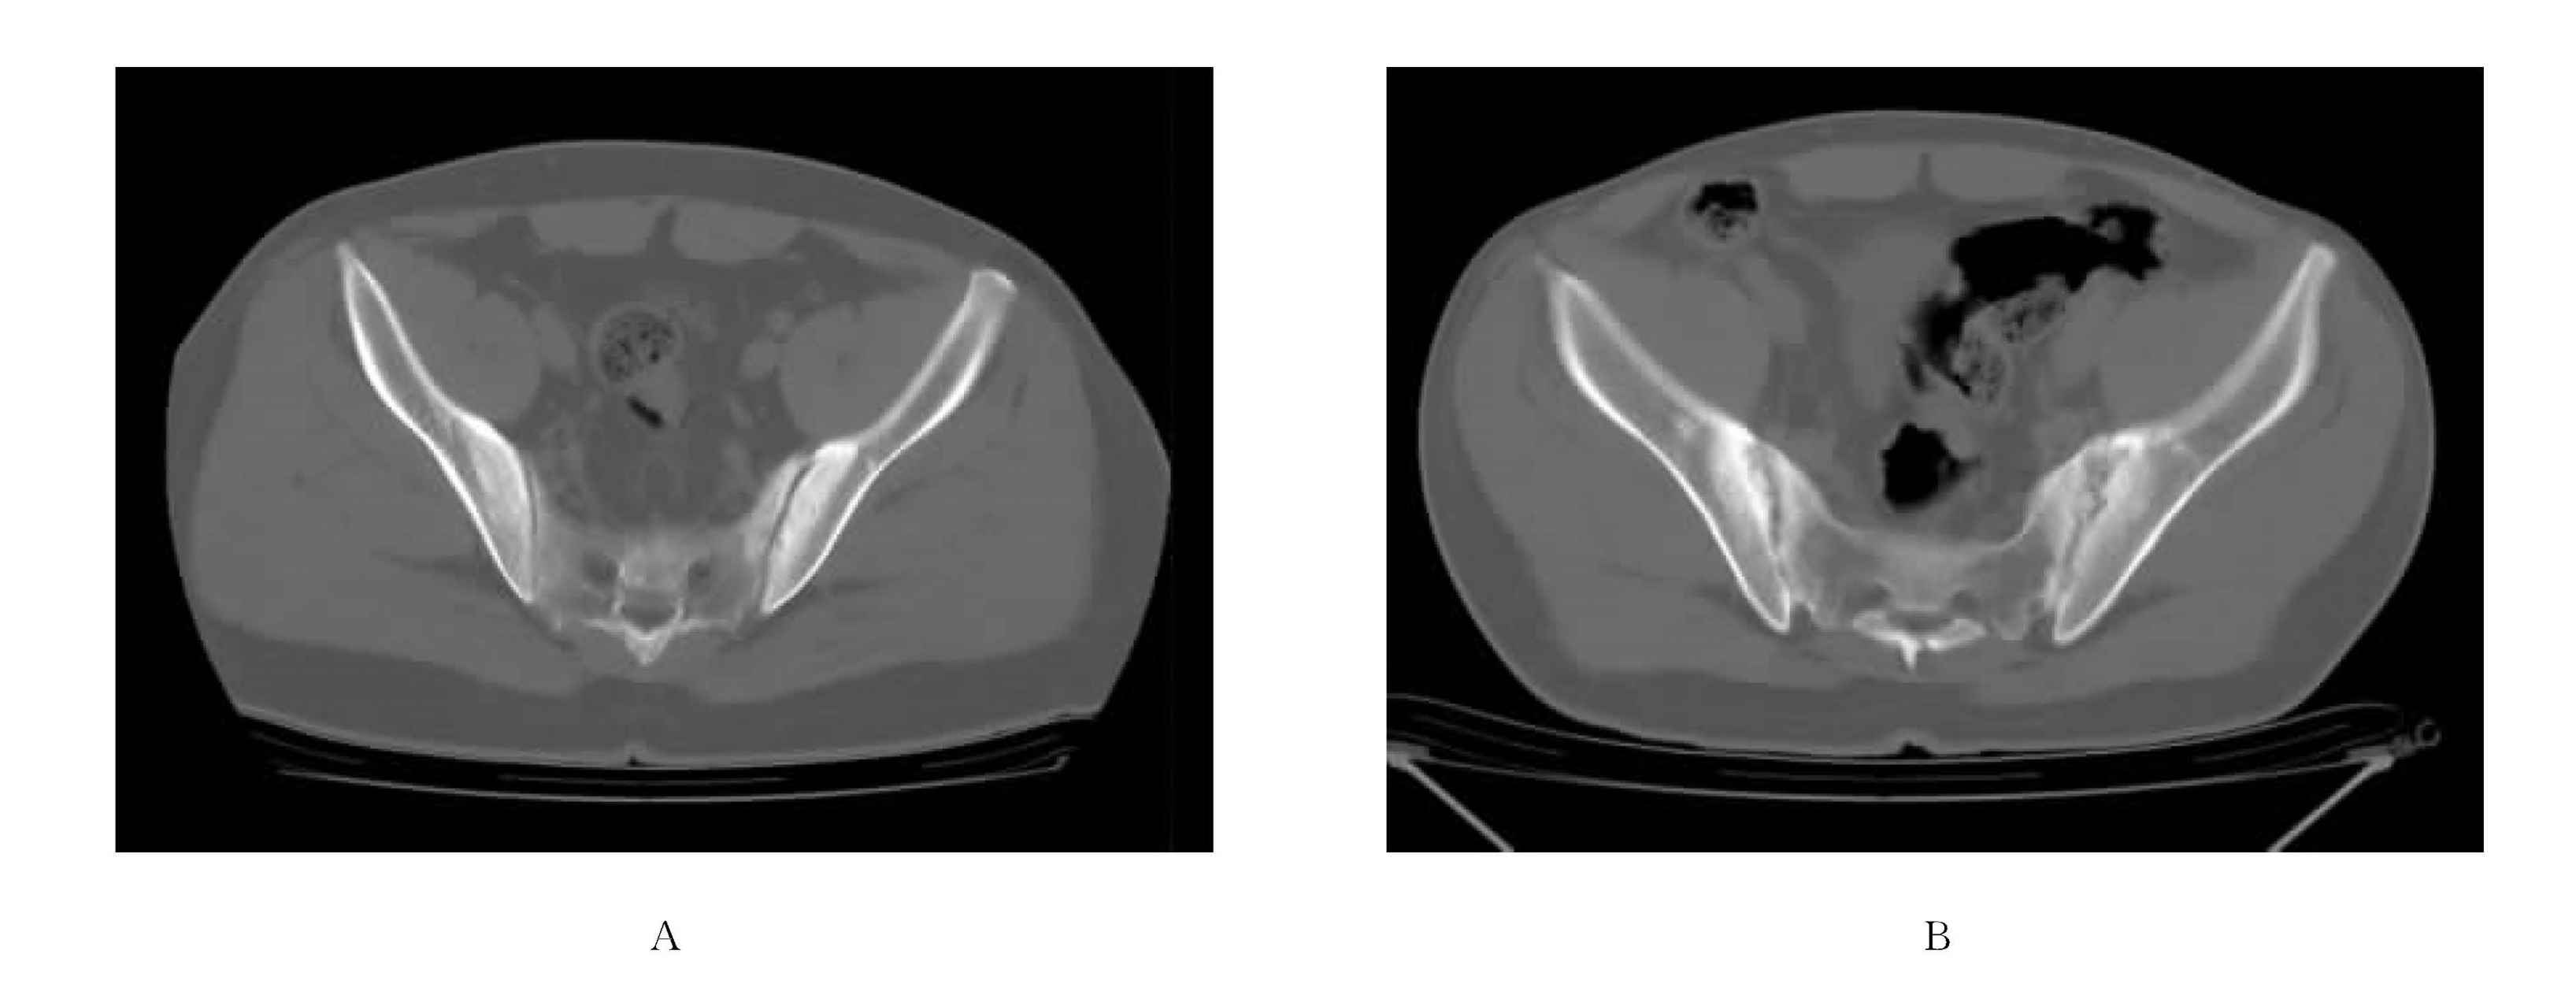
\includegraphics[width=.7\textwidth,height=\textheight,keepaspectratio]{./images/Image00455.jpg}
 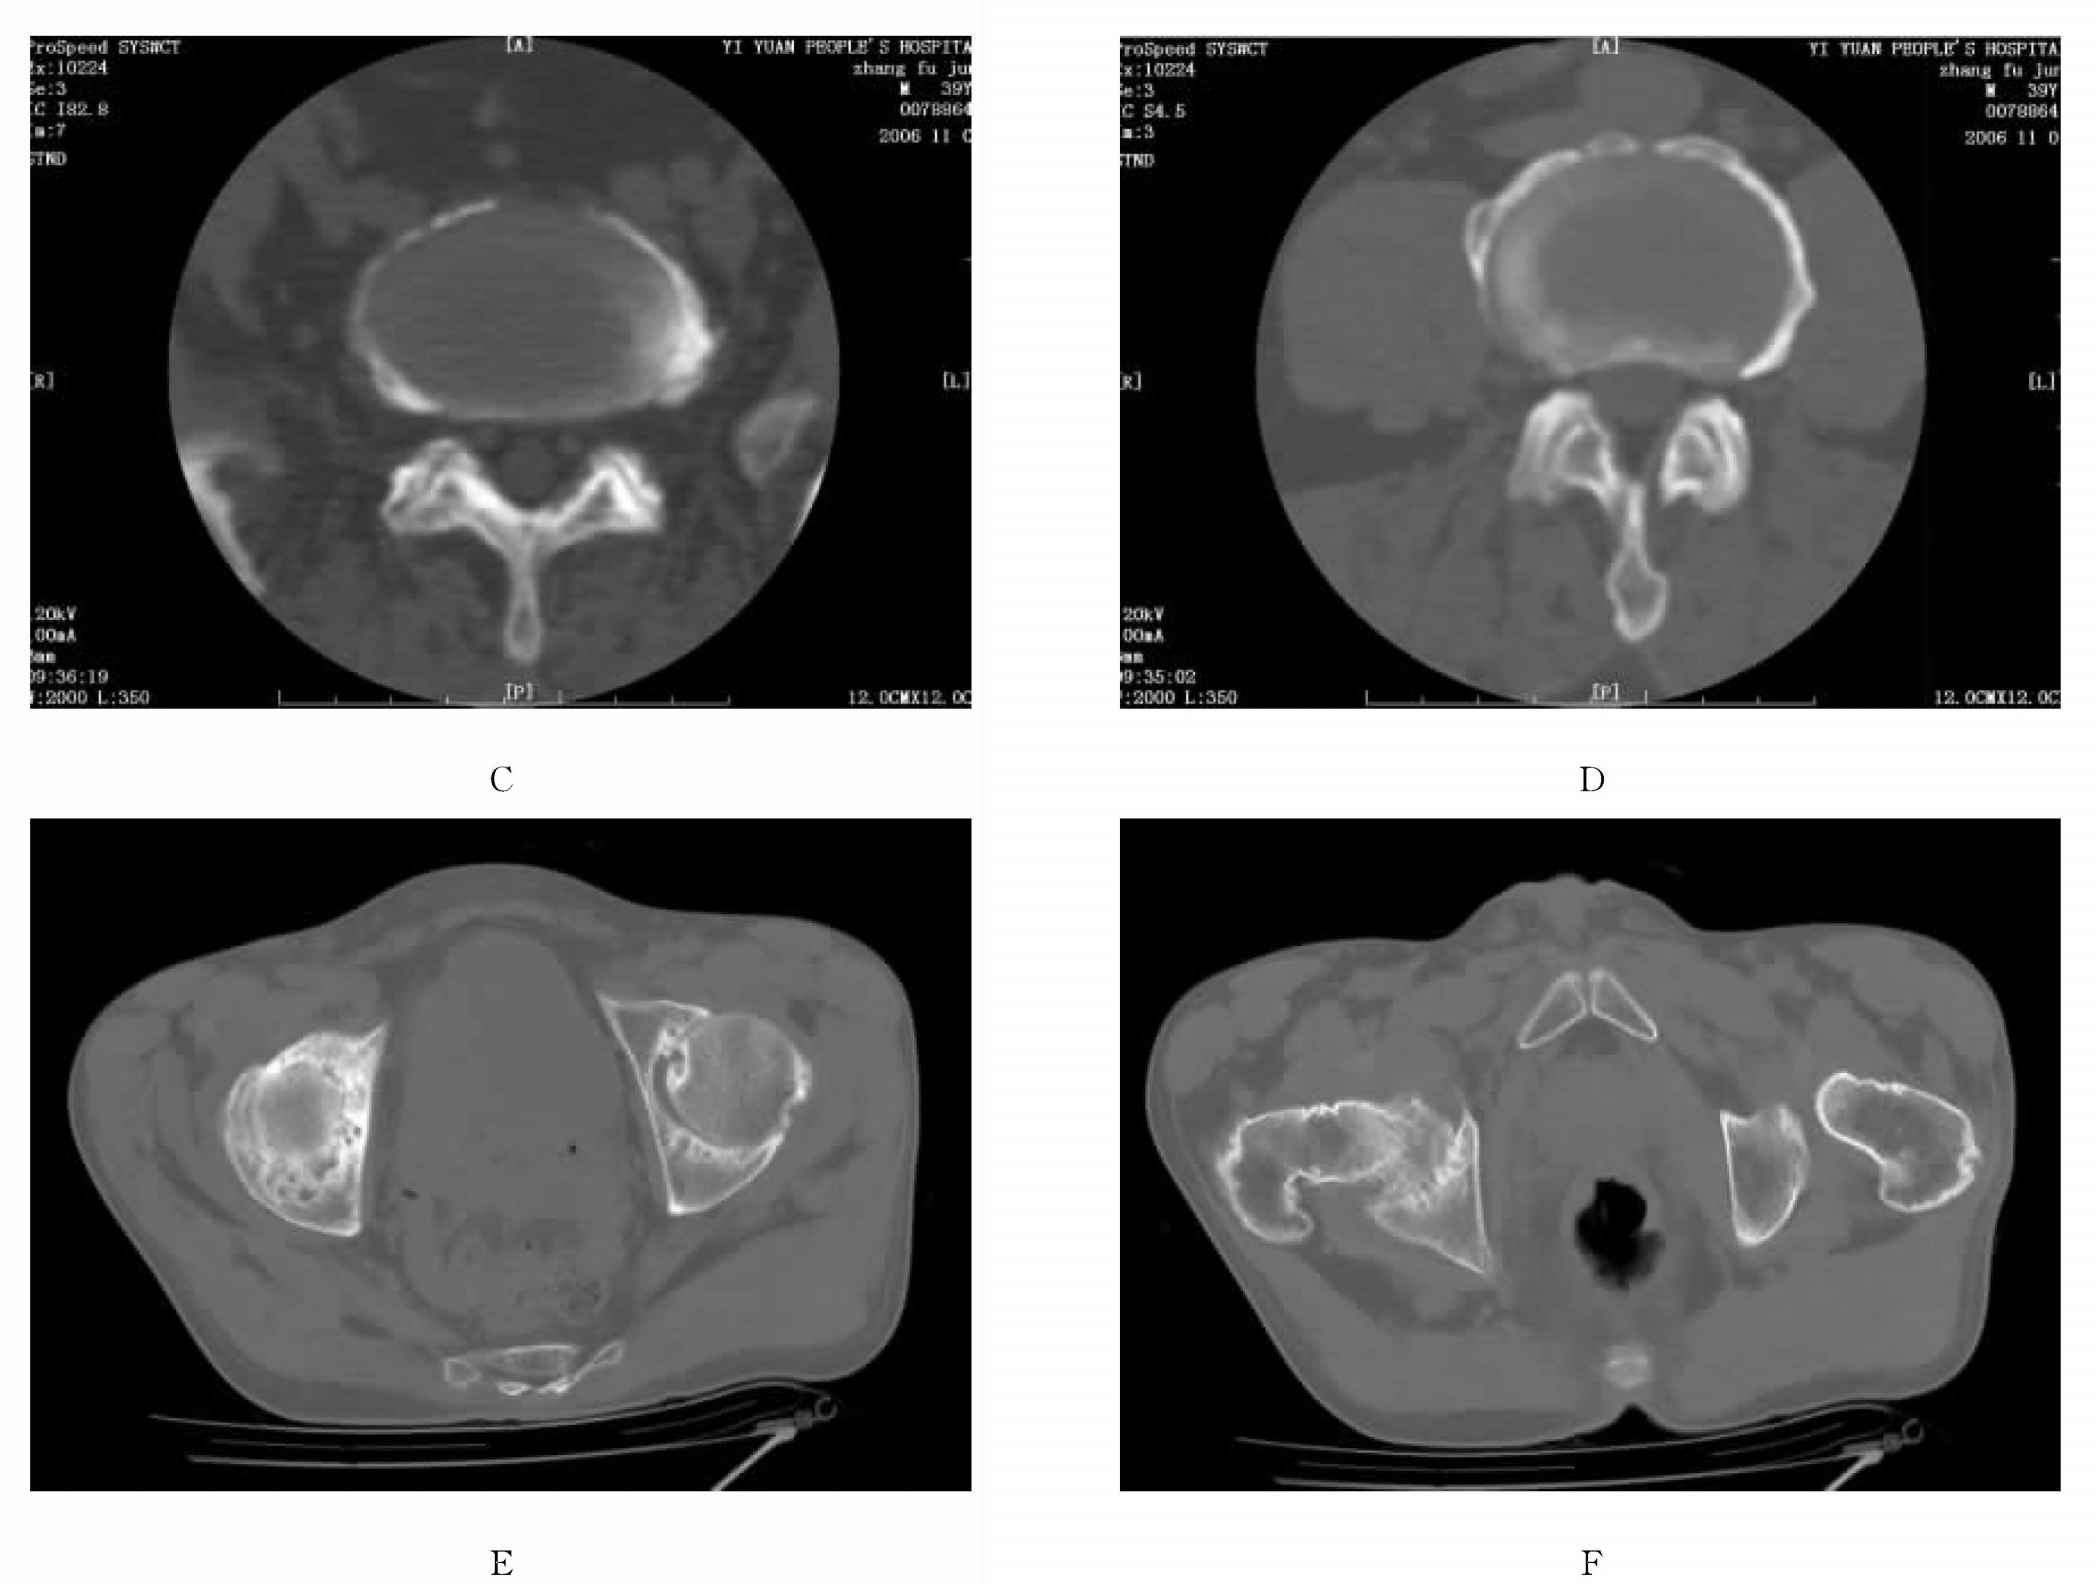
\includegraphics[width=.7\textwidth,height=\textheight,keepaspectratio]{./images/Image00456.jpg}
 \captionsetup{justification=centering}
 \caption{强直性脊柱炎\\{\small A为骶髂关节炎Ⅱ级表现,髂骨侧骨皮质局限硬化,关节面模糊、毛糙和软骨下微小囊变,左侧为著;B为骶髂关节炎Ⅲ级表现,软骨下骨质明显侵蚀破坏和弥漫性硬化;C示椎间小关节模糊,基本消失;D示前纵韧带广泛钙化骨化;E左右髋关节间隙变窄、关节面囊状侵蚀;F示左右股骨颈关节囊附着区、大粗隆骨质虫蚀样破坏(C、D为同一患者,E、F为同一患者)}}
 \label{fig22-30}
  \end{figure} 

总之,放射学对骶髂关节改变以及附着病的正确分析是AS早期诊断的关键。

2.骶髂关节改变的CT特点

(1)累及部位:骶髂关节病变以双侧,且以关节滑膜部(下2/3)髂骨侧受累多见。

(2)软骨钙化及关节间隙改变:表现为滑膜部关节间隙中与关节面穿行(横行)的高密度影(穿透性钙化),均由髂骨侧向骶骨侧发展。因关节滑膜只覆盖于关节边缘并不覆盖于关节软骨上,故国内有学者认为这种穿透性钙化是关节软骨钙化而非滑膜钙化。关节间隙可狭窄或增宽。

(3)关节面及其下骨结构的改变:关节面毛糙、高低不平或穿凿样破坏。①关节面下骨质吸收,明显的骨吸收可致原有骨性关节面呈条状高密度影;②骨吸收外侧骨质增生硬化;③关节面囊样改变,周围有环状硬化;④邻近骨质疏松。

(4)骶髂关节韧带部的韧带钙化。

3.骶髂关节炎的CT分级

目前尚无统一分级标准,参照X线分级可分为5级。0级:正常,关节面光整,间隙无变形。Ⅰ级:关节面模糊,骨皮质连续性欠佳,无关节面囊性变,无骨破坏、硬化增生,无关节间隙改变。Ⅱ级:骨皮质局限硬化,关节面模糊不清和斑块状脱钙,软骨下侵蚀、毛糙和软骨下微小囊变,关节间隙基本正常。上述异常始于髂骨面,骨质侵蚀和囊变最常见于关节中下部,很少累及韧带部。Ⅲ级:软骨下骨质明显侵蚀破坏和弥漫性硬化,关节面呈毛刷状和锯齿状,骨质疏松和囊变亦明显增多,关节间隙呈不规则狭窄或宽窄不均,可有部分强直。Ⅳ级:骶髂关节骨性强直,普遍骨质疏松,韧带部侵蚀和囊变更常见、更明显。

\textbf{【鉴别诊断】}
骶髂关节病变的病因可有血清阴性关节炎[包括强直性脊柱炎、Reiter综合征、牛皮癣关节炎、肠病性骨关节病(包括溃疡性结肠炎、Crohn氏病、Whipple氏病、沙门菌肠炎、小肠吸收不良综合征等)等]、类风湿性关节炎、化脓性关节炎、关节结核、退行性骨关节病、致密性骨炎、痛风性关节炎、复发性多软骨炎、肾性骨病、代谢性骨质软化、甲状旁腺功能亢进、布氏杆菌性关节炎、长期血液透析等。

AS之骶髂关节改变应注意与上述疾病相鉴别,还应注意与儿童骶髂关节的正常表现相鉴别。典型的AS常见双侧骶髂关节对称性受累且以下2/3为主,并逐渐累及腰椎小关节。

1.类风湿性关节炎:女性多于男性,以累及外周小关节为主。CT表现:骶髂关节受累多为单侧,以关节上部受侵多见,早期关节面下骨质疏松,继而出现小囊状骨质破坏。

2.感染性骶髂关节炎:多单侧,常伴明显的全身症状。CT可有关节间隙的增宽或狭窄,骨质破坏、增生,其周围软组织肿胀显著。

3.致密性髂骨炎:多见于经产妇。CT表现为髂骨的均匀性硬化,无骨质破坏及关节间隙改变,无软组织肿胀,骶骨一般不受累。

4.肠炎性骶髂关节炎的脊柱改变与AS相似,两者有相关性,需结合临床鉴别。

5.其他如牛皮癣关节炎、Reiter综合征等虽有脊柱改变,但其增生的骨赘是不连续、不对称的(而AS增生的骨赘连接于椎体间,呈对称性),且骶髂关节并非一定有改变,即便有改变亦不像AS那样典型,而呈不对称性。

6.正常儿童的骶髂关节(正常青少年骶髂关节的CT解剖特点见本章第二节):其髂骨侧关节面有囊样改变或局限性凹陷,皮质完整,但周围无硬化;骶骨侧关节面有骨侵蚀样改变,但周围无硬化,尤其髂骨侧关节面正常者不能诊断为骶髂关节炎。而强直性脊柱炎所致骶髂关节炎,其骨侵蚀的边缘有硬化,侵蚀灶主要位于髂骨面,没有仅侵蚀骶骨侧皮质者。

上述其他疾病的骶髂关节改变亦不像AS那样典型,且呈非对称性。结合临床不难鉴别。

\subsection{髂骨致密性骨炎}

致密性骨炎亦称为浓密性骨炎,系一种发生于髂骨、骶骨、椎体(L\textsubscript{4}
、L\textsubscript{5}
的上缘多见)、耻骨联合附近、跟骨、趾骨或股骨下端靠近关节边缘部的骨质硬化性疾病。

\textbf{【病因病理】}
病因未明。可能与身体负重劳损、血液供应异常、分娩期外伤、青年性驼背、慢性感染等有关。病理只是正常骨量的增多。

\textbf{【临床表现】}
髂骨致密性骨炎好发于20~25岁青年人,女性为男性的5~9倍,经产妇占绝大多数。站立位工作者发病率较高。主要表现为腰背部、骶髂部、耻骨联合处轻度疼痛,劳动后加重。

\textbf{【影像学表现】}
主要表现为髂骨耳状面中下2/3处有三角形、新月形或梨形均匀性高密度区。其内缘以骶髂关节为界,从不侵及关节。外缘多清晰,亦可边缘模糊逐渐移行于正常骨质中。病变可单侧或双侧先后发病。根据上述特点不难与AS相鉴别。

正常骶髂关节的髂骨侧有一生理性密度增高区,其形态近三角形,因很小X线不能显示,CT可予显示,它是通过躯干到下肢承受压力的反应。无论什么原因使该区压力增高,都能使该区增大,但仍保持其三角形形状,故髂骨致密性骨炎多呈三角形。

\subsection{退行性骨关节病}

本病可分为原发性和继发性,为软骨变性所致的关节病变。创伤性关节炎亦实为继发性退行性骨关节病。

\textbf{【病理】}
主要开始于关节软骨的退行变性,软骨退化变性后,机体的代偿修复使软骨下骨质增生,形成关节边缘骨赘和关节面增厚、硬化、变形。损坏变性的关节软骨可形成一个个小的陷窝和洞穴,滑液由此进入,在关节面下和骨内形成假囊肿。经常磨损使软骨、骨质碎裂甚至增生化生的滑膜脱落形成关节游离体。关节囊肥厚、纤维化。

\textbf{【临床表现】}
原发性骨关节病常见于老年人,发病缓慢,好发于髋、膝、脊柱及指间关节等,以关节活动不灵便、疼痛为主要症状,可有关节肿胀、积液表现。骶髂关节病变平片易被漏诊。

\textbf{【影像学表现】}
诊断要点为:关节间隙的不对称性狭窄、关节面硬化和变形、边缘性骨刺和骨桥、关节面下假囊肿及关节内游离体等,关节周围可有钙化(图\ref{fig22-31}、图\ref{fig22-32})。

\begin{figure}[!htbp]
 \centering
 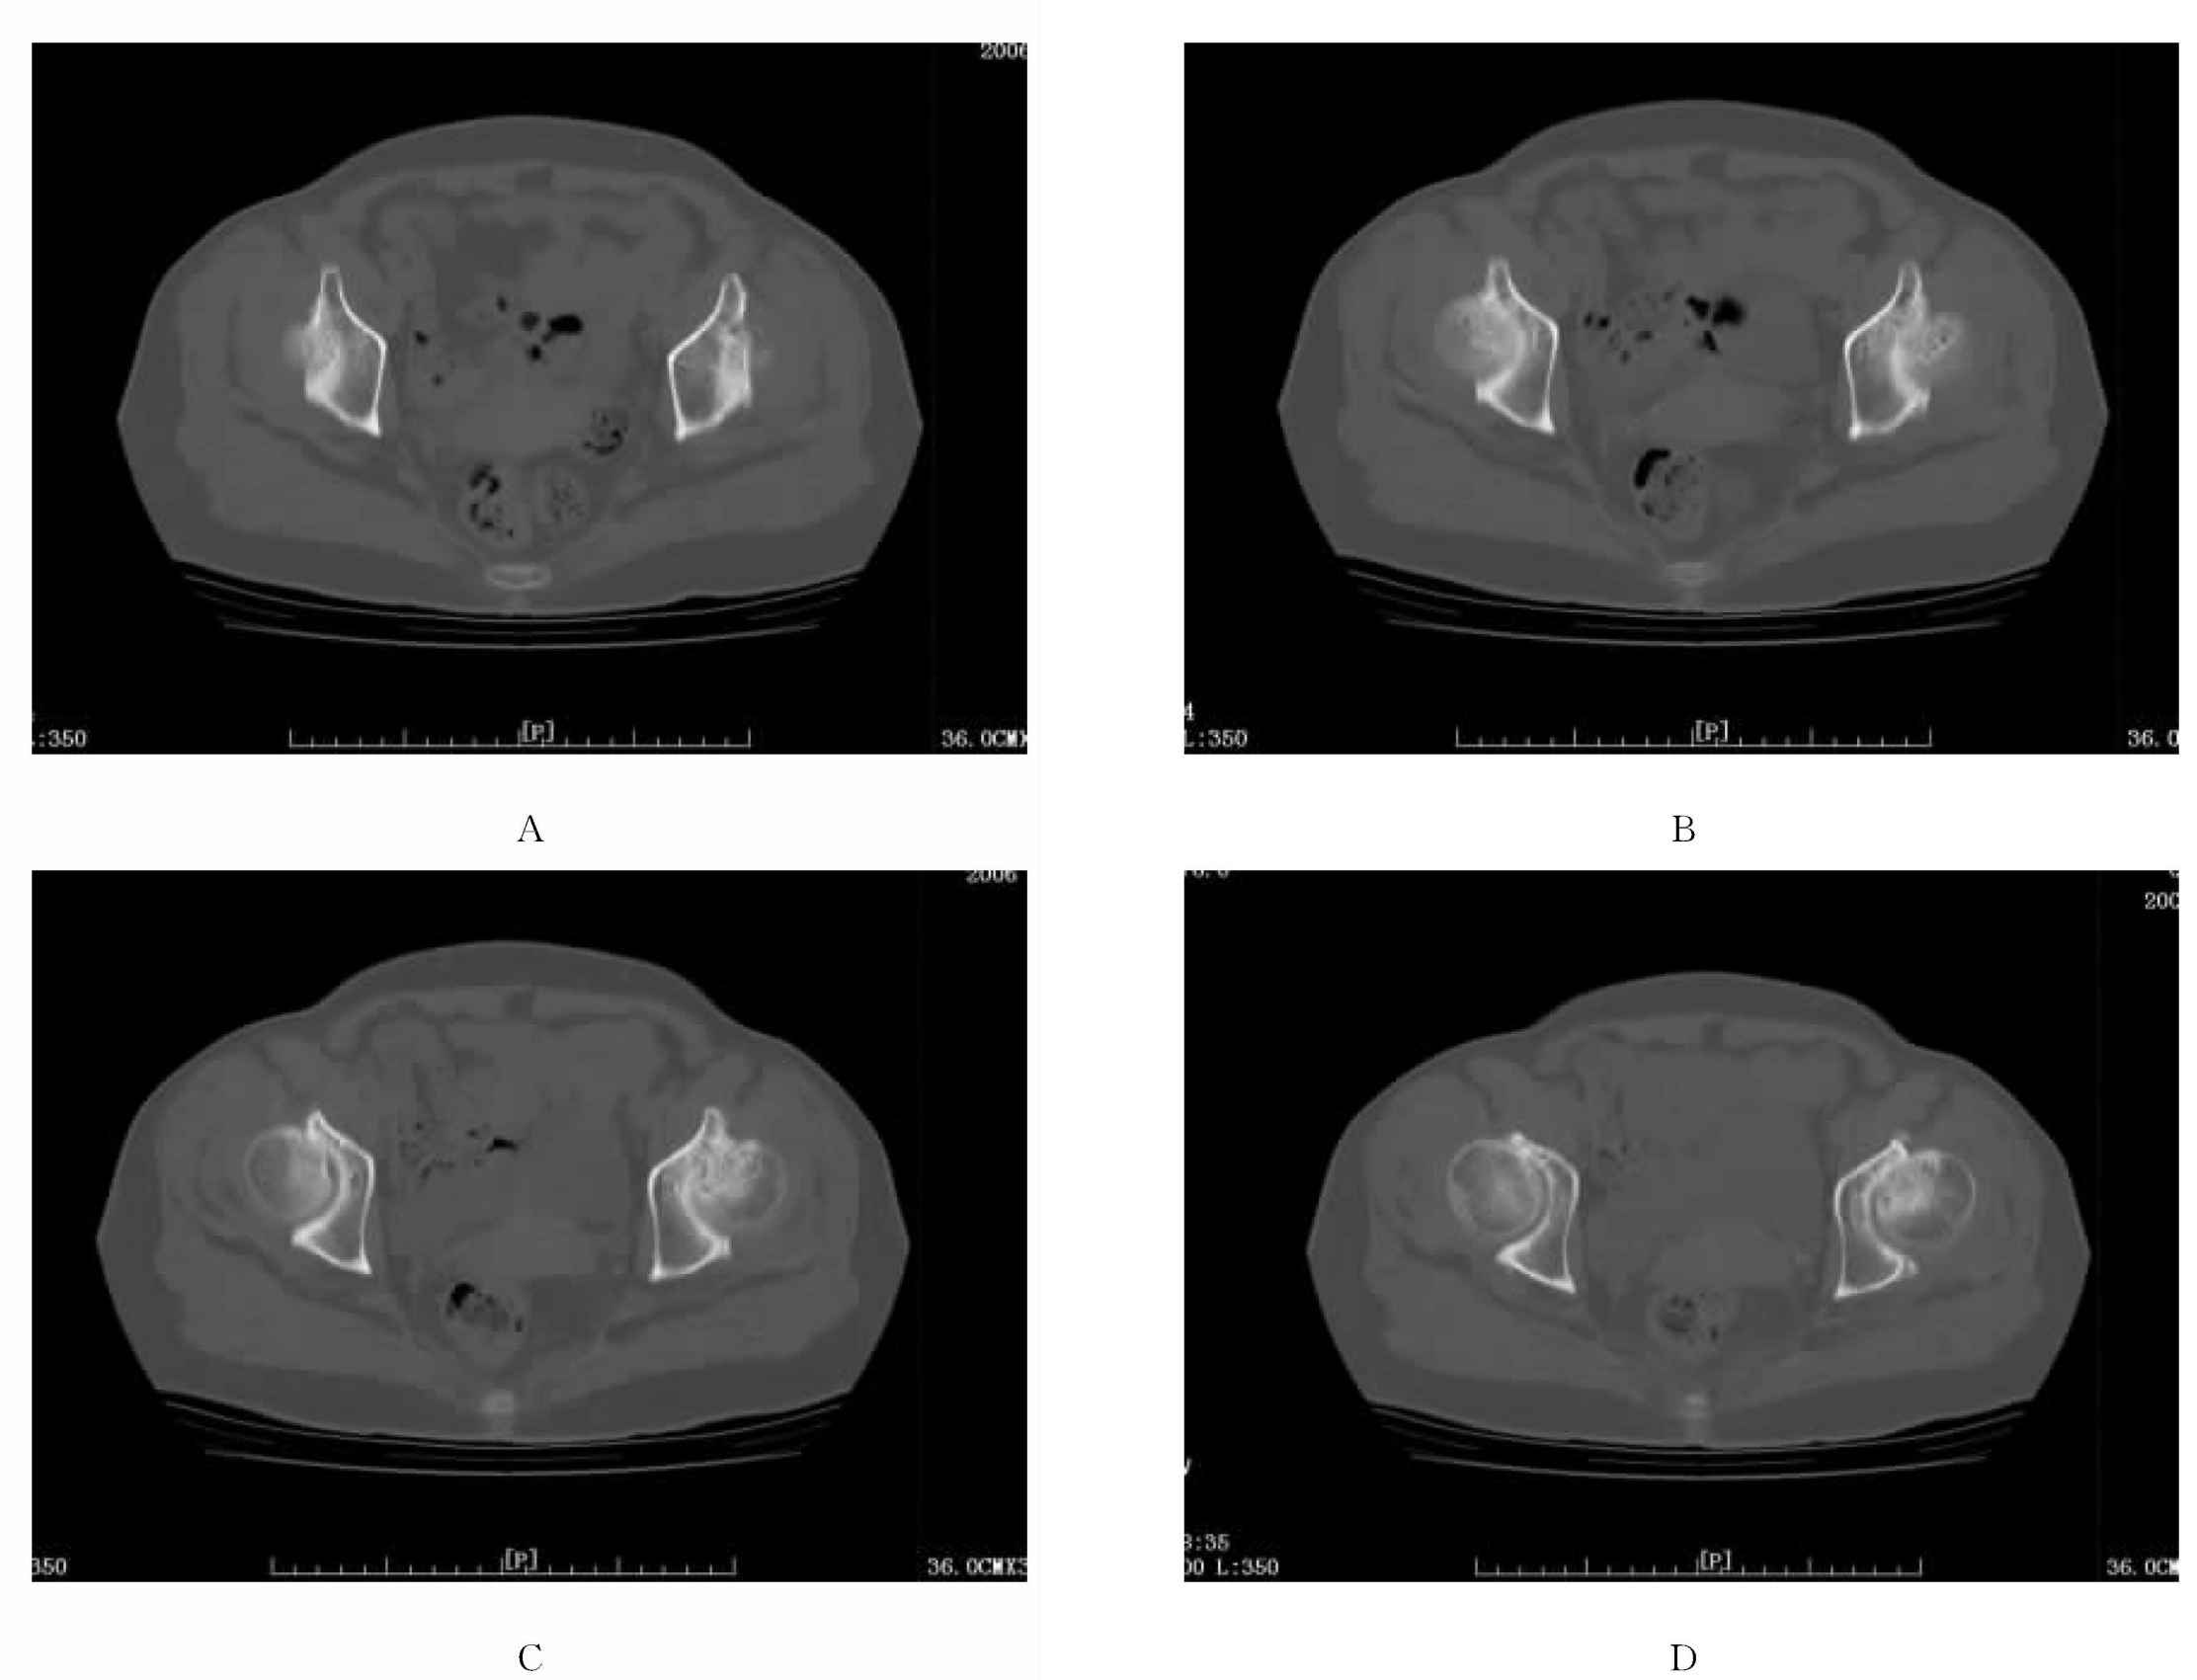
\includegraphics[width=.7\textwidth,height=\textheight,keepaspectratio]{./images/Image00457.jpg}
 \captionsetup{justification=centering}
 \caption{退行性髋关节病\\{\small A~D为同一患者,为髋臼发育不良所继发。左右髋臼浅平,不能包绕股骨头的顶部;髋臼边缘硬化,股骨头负重部硬化、囊变;关节间隙不对称狭窄}}
 \label{fig22-31}
  \end{figure} 

\begin{figure}[!htbp]
 \centering
 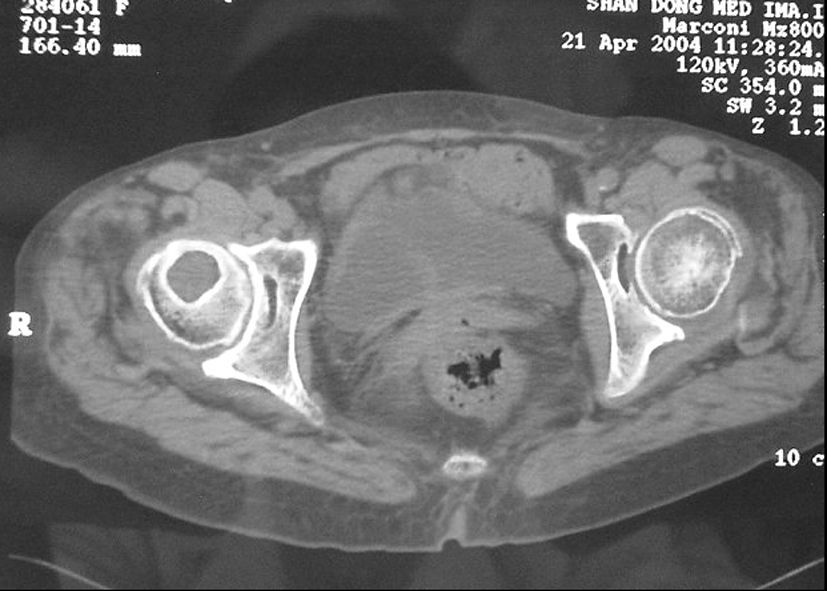
\includegraphics[width=.7\textwidth,height=\textheight,keepaspectratio]{./images/Image00458.jpg}
 \captionsetup{justification=centering}
 \caption{关节面下假囊肿\\{\small 右侧股骨头关节面下有圆形囊状低密度灶,边缘硬化;髋关节面增生硬化}}
 \label{fig22-32}
  \end{figure} 

本病的软骨下变化可分为两期。①破坏期:以骨硬化和囊肿形成、骨性关节面变扁变形为特点,且以关节负重部显著,但无明显破碎、节裂表现,据此多可与缺血坏死尤其是股骨头缺血坏死相鉴别。②形成期:以关节非持重部有明显骨质增生为特点。

\subsection{色素沉着绒毛结节性滑膜炎}

本病为慢性关节病变,以关节滑膜高度增生、绒毛结节形成伴含铁血黄素沉着为特点。

\textbf{【分型】}
根据解剖部位可分为关节型、腱鞘型、滑囊型。根据病变范围又可分为弥漫型和局限型。弥漫型又称为弥漫性腱鞘巨细胞瘤,多见于大关节。局限型又称为腱鞘巨细胞瘤、结节性滑膜炎、滑膜纤维组织细胞瘤等,主要见于手足小关节。

\textbf{【病因病理】}
病因有炎症、肿瘤、外伤关节出血、代谢障碍、变态反应及感染等学说。现多认为本病具有炎症及肿瘤双重性质,由炎性增生逐渐过渡到瘤样增生,两者之间无明显界限。

病理以弥漫型较多见,与局限型的组织学表现完全一样,但肉眼所见却不相同。弥漫型可见滑膜不规则增厚,长满大小不等的棕色结节或细长绒毛,结节可有蒂或无蒂;局限型则以滑膜单个结节状肿块为特征。本病有恶性变和远处转移的报道。

\textbf{【临床表现】}
多见于青壮年,20~40岁占80%,男女之比约2∶1。发病部位以膝关节多见,其次为髋、踝、跗等关节,上肢关节少见。临床起病缓慢,半数以上有外伤史。早期无症状,逐渐出现疼痛、肿胀、关节积液、关节功能障碍、关节绞锁等表现。可触及局限性肿块,扪之如海绵,关节抽液呈巧克力色。

\textbf{【CT表现】}
①关节积液,密度较一般非血性液体密度高,CT值一般20~40Hu。②平扫时因增厚的滑膜或结节与血性积液的密度相近,因此难以显示。增强扫描呈关节腔内单个或多个强化的软组织结节影或滑膜不规则增厚伴关节积液是本病的特征性表现。③可见跨关节的骨质侵蚀破坏,边缘光滑,病变侵入骨内(关节面下)呈小囊状、虫蚀状,边缘锐利并有硬化,很少侵蚀关节面(图\ref{fig22-33})。一般无骨膜反应,可有一定的骨质疏松。④可继发退行性变。

\begin{figure}[!htbp]
 \centering
 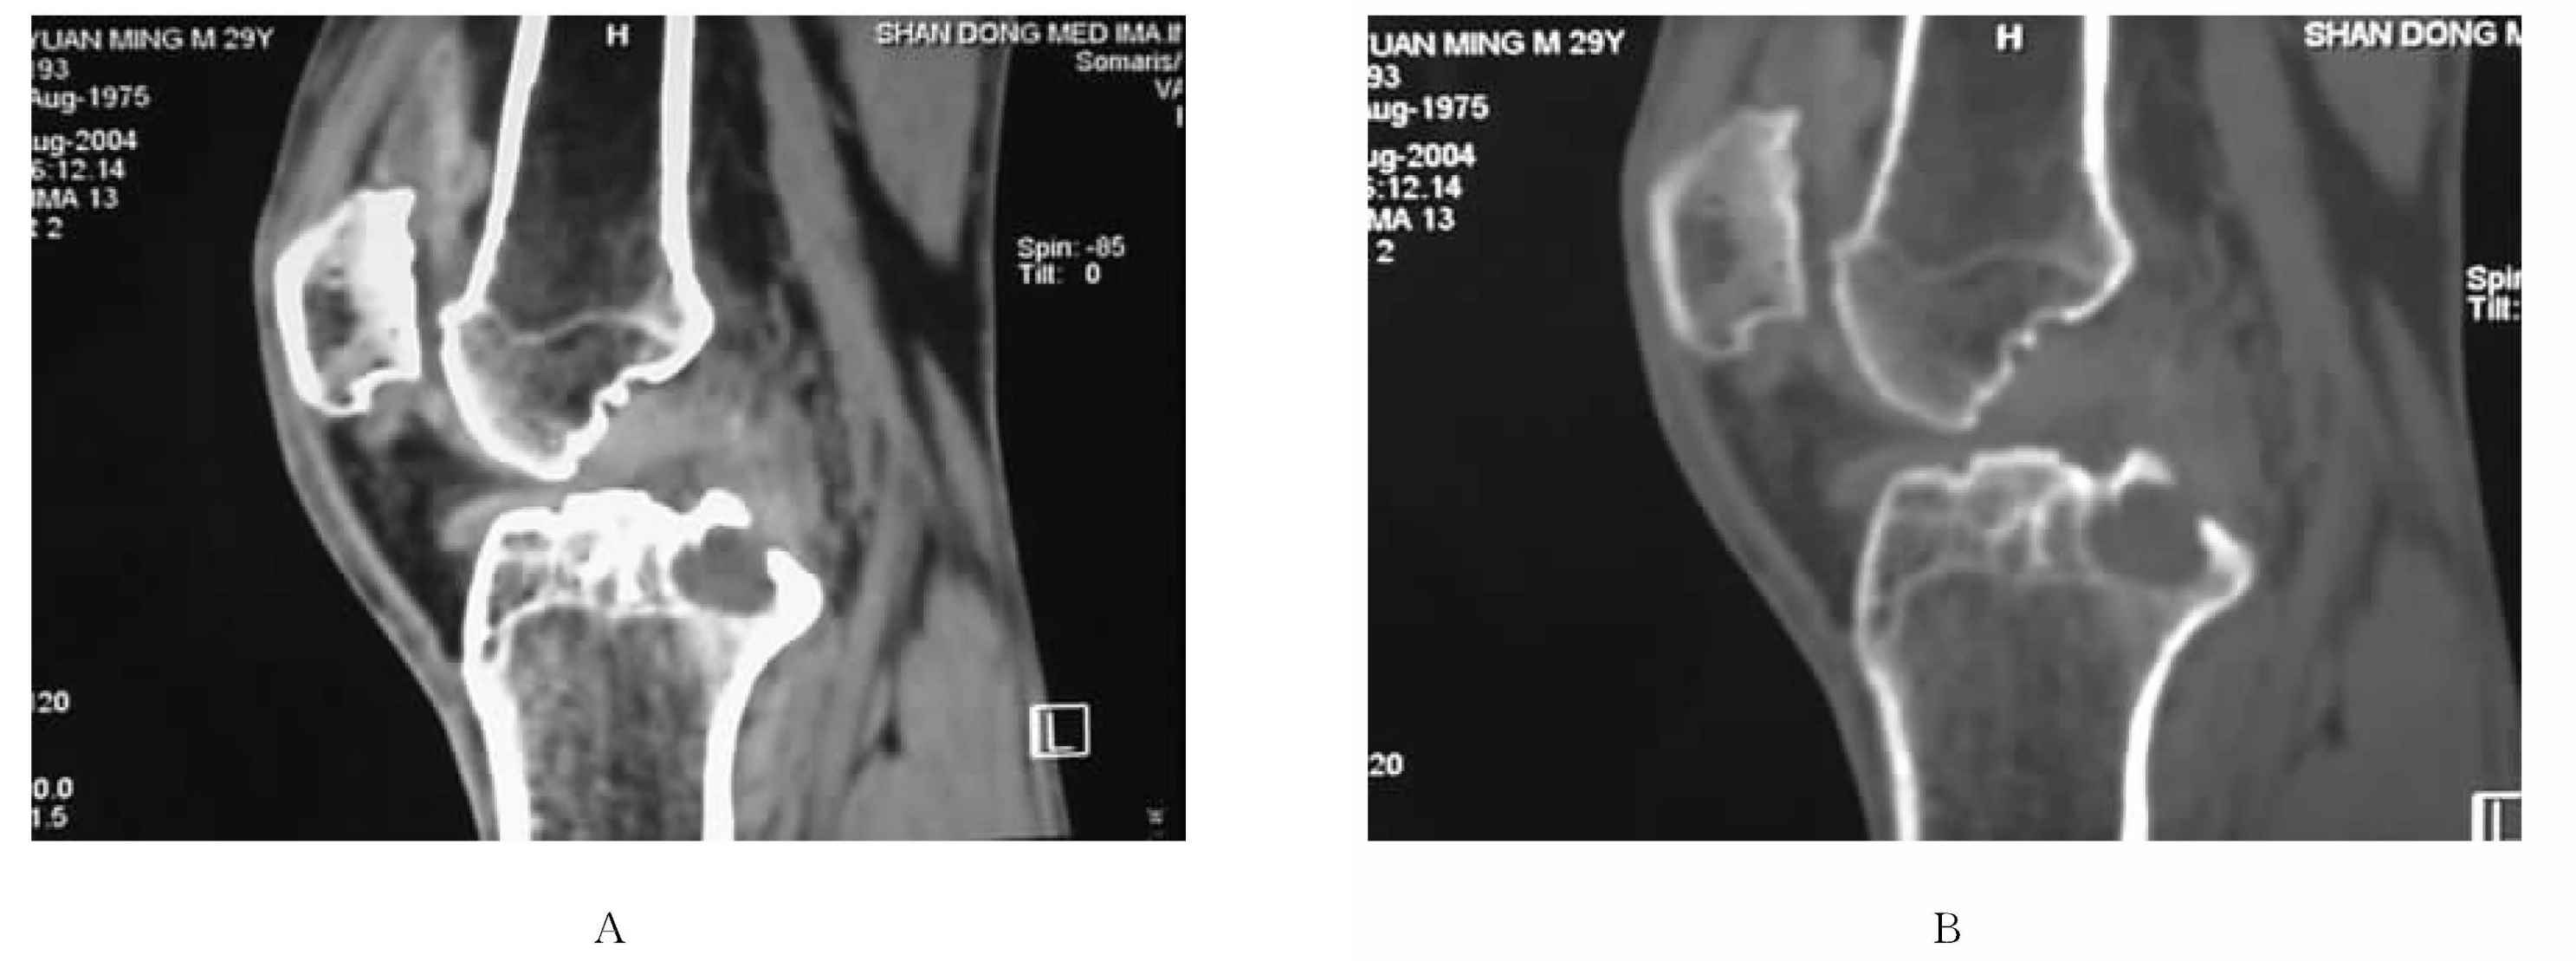
\includegraphics[width=.7\textwidth,height=\textheight,keepaspectratio]{./images/Image00459.jpg}
 \captionsetup{justification=centering}
 \caption{色素沉着绒毛结节性滑膜炎\\{\small 右膝关节内滑膜广泛不规则增厚和软组织结节影;可见跨关节的骨质侵蚀破坏,关节面受侵}}
 \label{fig22-33}
  \end{figure} 

\textbf{【鉴别诊断】}

1.创伤性骨关节炎、关节结核、化脓性关节炎及血友病等均可有滑膜增厚,通常是均匀一致的,更无结节状改变。

2.类风湿性关节炎可有滑膜不均匀增厚,但一般无明显的结节形成;骨质疏松较明显,关节面下骨吸收以多个小囊样低密度影为特点。结合临床不难鉴别。

\subsection{滑膜骨软骨瘤病}

本病主要发生于具有滑膜组织的关节囊、滑囊和腱鞘,以滑膜面形成软骨性或骨软骨性小体为特征。

\textbf{【病因病理】}
本病病因不明。一般多支持化生学说,即滑膜本身有潜在的造骨功能,当受到各种刺激时,滑膜深层未分化的间叶细胞分化为软骨体,再通过软骨内化骨形成骨软骨体,乃称为滑膜骨软骨瘤病。

病理可见滑膜增生肥厚,表面分布大小不等的软骨或骨软骨体。软骨体从中心开始骨化,所以骨软骨体中心为骨组织,外部为软骨组织,周围为纤维组织与滑膜相连接。骨软骨体一旦脱落游离于关节腔与滑膜血管中断后,即停止骨化。由于滑液的营养,软骨的表层可能有少量增生。软骨体的表层为生长层,中层为软骨细胞增生肥大层,深层为软骨基质钙化层。来自滑膜的血管侵入钙化层而后成骨。

\textbf{【临床表现】}
多见于青壮年男性。多数单关节发病,最常受累的关节是膝关节,其次是髋、肘、踝、肩和腕关节。主要表现为受累关节疼痛、肿胀和活动受限,也可无症状,很少出现关节绞锁现象。

\textbf{【影像学表现】}
早期表现为软组织肿胀、滑膜不规则增厚;进展期呈大小一致的、多<1cm的骨软骨体;晚期继发退行性变,骨软骨体多>1cm。①骨软骨体可小如针尖、大如鸭蛋;数目少则几个,多则千余个。②形态呈圆形或椭圆形;有的聚集成堆,有的散在分布。③典型者中心浅淡稀疏,周边有一浓密硬化环,前者由松质骨构成,后者系软骨基质钙化层。④约1/3软骨体无钙化骨化,需结合关节造影确诊。⑤常继发关节退行性变。

\textbf{【鉴别诊断】}

1.退行性骨关节病:其关节游离体较小、较少,且缺少硬化环,有时不易鉴别。有学者认为骨性游离体超过4个即可诊为滑膜骨软骨瘤病,对此需进一步探讨。

2.剥脱性骨软骨炎:通常只有一个游离体,且邻近关节面有局限缺损。

3.神经营养性骨关节病:以关节无痛性肿大、关节结构严重破坏紊乱、半脱位及邻近散在不规则碎骨片为特征。

4.色素沉着绒毛结节性滑膜炎:其滑膜增厚远较滑膜骨软骨瘤病显著,但后者无骨质破坏且有特征性的骨软骨体而不难鉴别。

\subsection{邻关节囊肿}

本病又称为邻关节骨囊肿或骨内腱鞘囊肿,也有人曾称为骨内滑膜囊肿、软骨下囊肿或骨内黏液囊肿等。

\textbf{【病因病理】}
本病病因病机不明。①邻近软组织腱鞘囊肿或骨膜腱鞘囊肿向骨内侵蚀穿透形成,但该类少见;②骨内成纤维细胞化生、增殖并分泌黏液压迫骨质所形成;③骨表面机械性应激反应和反复轻微损伤引起骨内血液循环障碍而发生黏液变性;④外伤及骨折后,滑膜经外伤性缺损的关节软骨疝入骨内形成囊肿。

病理表现病灶为单房或多房,纤维组织包膜厚薄不均,囊内充满黏稠的白、黄色胶冻样物。液体浓缩干枯、蛋白组织释出氮气可形成囊内真空现象。镜下可见包膜由束状胶原纤维构成,有少量成纤维细胞。覆盖囊腔内面的扁平细胞似滑膜,但不见连续的滑膜层。

\textbf{【临床表现】}
发病年龄13~65岁不等,多见于青、中年。临床症状缺乏特征,表现为局部酸痛或不适,运动或体力活动时加重,病程通常较长。

\textbf{【CT表现】}
好发于长骨(特别是下肢)的骨端如股骨头、股骨远端、胫骨近端和内踝附近等。不规则骨可见于髋臼外上缘、腕骨、距骨、肩胛盂附近、髌骨、手足短管骨等。表现为邻近关节的圆形、椭圆形囊状低密度,大小1~5cm,常偏心分布。邻近皮质膨胀变薄,可有小段裂隙。病灶一般小的为单房、大的可多房,边缘薄层硬化,也可有骨嵴或斑状硬化(图\ref{fig22-34})。病灶可为软组织或水样密度,含有液体和气是其特征。无显著的关节退变表现。

\begin{figure}[!htbp]
 \centering
 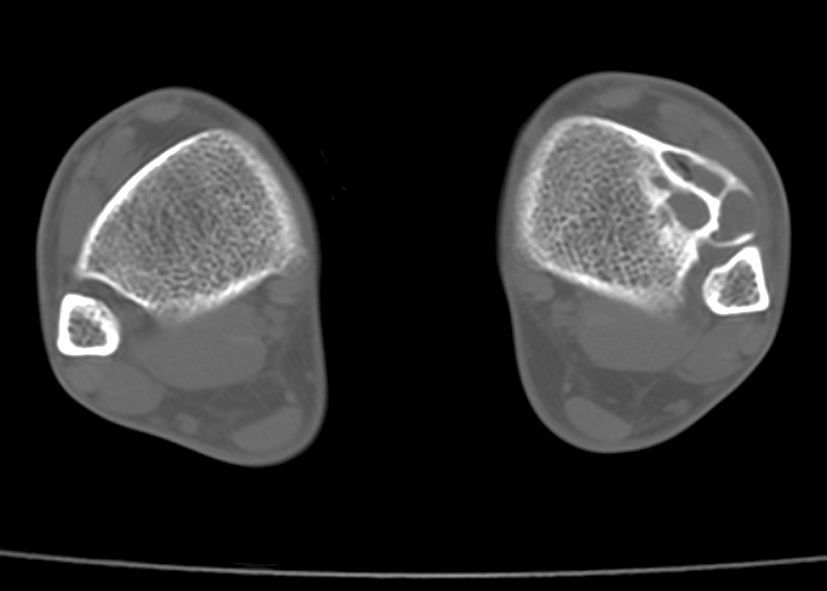
\includegraphics[width=.7\textwidth,height=\textheight,keepaspectratio]{./images/Image00460.jpg}
 \captionsetup{justification=centering}
 \caption{邻关节囊肿\\{\small 左侧胫骨远端邻近关节的多房囊状低密度灶,偏心分布,边缘薄层硬化,并有骨嵴}}
 \label{fig22-34}
  \end{figure} 

\textbf{【鉴别诊断】}
主要应与退行性骨关节病相鉴别。本病无关节间隙变窄和明显的骨质增生硬化等显著退变表现,是与后者鉴别的关键。

\subsection{股骨颈疝窝}

本病又称股骨颈滑膜疝,有文献将其作为正常变异论述。

\textbf{【病因病理】}
本病系关节滑膜侵蚀股骨颈前部皮质后,滑膜(液)疝入松质骨内形成。可能与前部关节囊与相邻的股骨头基底部、股骨颈近段外侧皮质间存在长期的压迫和相互摩擦有关。病理为致密的纤维结缔组织,可伴黏液样变。

\textbf{【临床表现】}
好发于中老年人。多无明显症状,偶有髋部轻微不适,多为偶然发现。

\textbf{【CT表现】}
多单侧发生,偶为双侧。位于股骨头基底部和股骨颈近段前侧皮质下、股骨颈中轴线外侧,偶位于股骨颈中部。呈圆形或椭圆形低密度区,边缘清晰且多伴薄层硬化,部分开口于关节腔(图\ref{fig22-35})。病灶最大径多<1.0cm,有文献报道可达3.0cm。

\begin{figure}[!htbp]
 \centering
 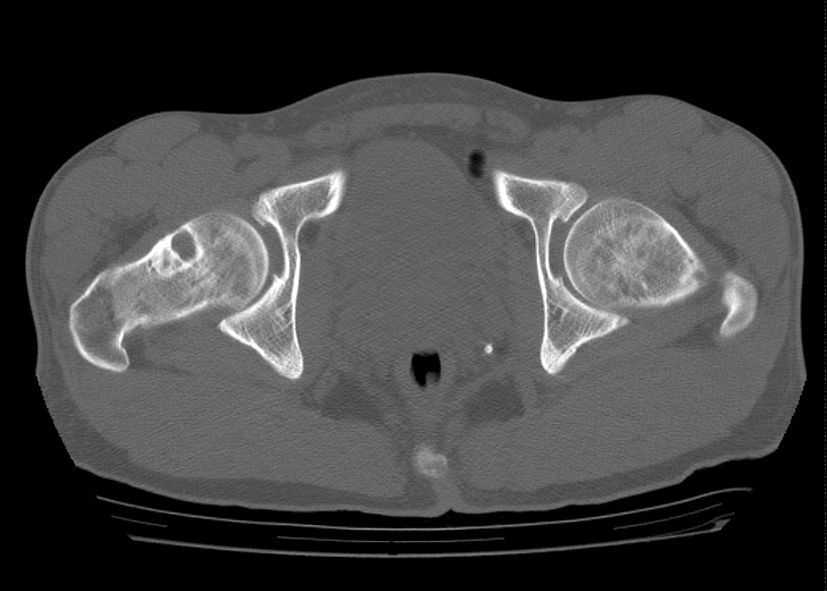
\includegraphics[width=.7\textwidth,height=\textheight,keepaspectratio]{./images/Image00461.jpg}
 \captionsetup{justification=centering}
 \caption{股骨颈滑膜疝}
 \label{fig22-35}
  \end{figure} 

右侧股骨颈近段前侧皮质下有椭圆形低密度灶,边缘有薄层硬化\textbf{【鉴别诊断】}
与骨内腱鞘囊肿(邻关节囊肿)临床、病理、影像学表现相似,发病位置是鉴别的关键。根据其特殊的位置,结合其他表现也不难与退变性囊肿、骨样骨瘤等相鉴别。

\section{骨缺血性坏死}

\subsection{概述}

\subsubsection{定义}

骨缺血性坏死又名骨无菌坏死、骨坏死、骨软骨病、骨软骨炎,是指骨组织失去血运导致骨内细胞成分的死亡及丧失新陈代谢的能力,通常发生于骨端或骨骺。骨缺血坏死亦包括骨梗死,是指血管阻塞所致的骨坏死,多为干骺和骨干的骨坏死。

骨缺血坏死好发于股骨头,亦可发生于全身关节骨骼如肩、膝、踝、腕关节。骨梗死常见于股骨远端、胫骨近端和肱骨近端,可单侧或双侧对称发病或见多发性病灶。

\subsubsection{病因}

1.外伤:关节内骨折或关节脱位。最常见于股骨颈、手舟骨、距骨颈骨折,其次为肱骨小头、肱骨头骨折,髋脱位、月骨脱位亦常见。

2.骨梗死:分为原发性和继发性。原发性少见,后者多见于潜水减压病和糖尿病等。

3.药物诱发:大量接受甾族化合物,应用皮质醇为抑制器官移植后的排斥,以及应用止痛剂。

4.物理性损伤:如放射性损伤、电烧伤、冻伤等最易发生坏死。

5.造血系统疾病:如血友病、红细胞增多症、血红蛋白病、镰状细胞性贫血、地中海贫血等。

6.常见综合因素:如酒精中毒、慢性胰腺炎、痛风、血尿酸过多、糖尿病、脂肪代谢障碍、结缔组织疾病等,以及少见的综合因素如反复轻微外伤、铁中毒、铜代谢障碍等。

7.儿童期发生骨缺血坏死称为骨软骨病,有文献亦将儿童期骨缺血坏死称为特发性骨缺血坏死,其他原因所致者为继发性骨缺血坏死。骨软骨病常见部位有:股骨头、胫骨结节、跖骨头、足舟骨、椎体以及少见部位的跟骨结节、髌下极等。除发生于跖骨和跟骨的缺血坏死以女性多见外,其余部位以男性多见。

\subsubsection{病理}

骨的血供不足有3种类型。①血流的中断:如创伤(骨折或脱位)后的血管破裂;②栓塞或沉积:如镰状细胞病、胰腺炎、减压病及血管炎等疾病;③骨内血管受压:如骨髓内成分增多和(或)骨髓腔内压力增高。

骨缺血坏死病理分为3期。①坏死期:骨细胞陷窝空虚,骨细胞消失。缺血导致造血组织在6~12小时死亡,破骨细胞、骨母细胞在12~48小时内死亡,骨髓脂肪在2~5天内死亡。②修复期:新生血管和肉芽组织向坏死组织内伸入形成节裂征象,逐渐清除死骨,在周围存活的骨髓内产生成骨活动。受累骨骼因负重而碎裂、变扁。③愈合期:坏死骨质消失,骨结构恢复正常,但可遗留畸形。

\subsubsection{影像学表现}

有学者通过羊的股骨头实验发现:①X线和CT
7周前不能反映股骨头缺血坏死的病理变化,12周后因骨细胞大量坏死、脱钙才发现骨密度下降和小梁结构紊乱。②MR在1周即可检出异常信号改变。

骨缺血坏死主要有下列放射学征象:①初期:为坏死期,坏死骨组织呈相对性骨密度增高,均匀一致。②中期:为坏死吸收期,局限性吸收的早期密度减低区并不明显;随后界限清晰,并逐渐形成囊状或带状骨质吸收,可见大片死骨游离;并随死骨的吸收低密度吸收区逐渐增大或相互融合。③晚期:为关节变形、骨质增生期,随着死骨的吸收,可发生病理骨折甚至关节面塌陷。

另一方面随着疾病的进展,在带状和囊状骨质缺损周围由于新骨形成,可见骨质增生硬化,即出现骨密度增高表现。小的囊状骨缺损可被新生骨充填;大的囊状骨缺损造成关节面塌陷者,则产生不均匀性骨质硬化。在长期的慢性恢复过程中可见关节边缘骨质增生,骨端呈蘑菇状变形,关节间隙增宽、狭窄或宽窄不均等退行性骨关节病表现。但是中、晚期变化亦合并存在,难以截然分开。

总之,骨缺血坏死主要表现为患骨骨端或骨骺体积变小、密度增高,有节裂、囊变或破碎征;关节间隙早期多增宽,晚期呈骨端变形及关节退行性变表现。

\subsection{成人股骨头缺血坏死}

本病近年来有日益增多的趋势,其发病率远远超过儿童股骨头骨骺缺血坏死。

\textbf{【病因病理】}
其病因很多,可达40余种,常见的有创伤、皮质激素治疗和酒精中毒。股骨头血供主要来源于股深动脉发出的旋股内侧动脉和旋股外侧动脉,两者在股骨颈基底部形成动脉环,因此关节囊内骨折会导致股骨头血供减少,易并发股骨头缺血坏死。也有相当一部分找不到明确病因。病理上自坏死中心部位到正常骨质区域可分为4个带:细胞坏死带、缺血损伤带、充血反应修复带及正常组织。

\textbf{【临床表现】}
好发于30~60岁男性,50%~80%的病人最终双侧受累。主要表现为髋部疼痛、压痛、活动受限、跛行,“4”字试验阳性。晚期关节活动受限加重,同时还有肢体缩短、肌肉萎缩和肢体屈曲、内收畸形。

\textbf{【影像学表现】}

1.基本征象

①股骨头均匀一致性密度增高:这一征象是骨折的直接反映,股骨头全部缺血坏死的肯定征象;②股骨头局限性疏松囊变:这一征象间接反映了股骨头局部缺血坏死的征象;③股骨头不均匀性骨质硬化:这种不均匀性硬化并不是骨的坏死区,而是新生骨区,间接反映了有分散的小片状骨坏死。

2.继发改变

①股骨头变形:可变小或变大;②髋臼增大;③关节间隙的改变:早期增宽,晚期变窄;④股骨头死骨再骨折:多见于股骨头全部缺血坏死;⑤关节软组织变化:关节囊肥厚,CT示其厚>6mm或呈波浪状不规则;⑥股骨头内气体:多见于股骨头塌陷者;⑦关节积液及髂腰肌囊扩张。

3.早期CT表现

其主要早期征象为正常星芒状结构变形,股骨头内单纯或交织存在的簇状、条带状和(或)斑片状高密度硬化(单纯硬化病变),边缘较模糊(图\ref{fig22-36}A)。

条带状硬化粗细不均,主要有3种走行方式:①沿正常股骨头星芒状结构,自股骨头中心向周围延伸;②与正常股骨头星芒状结构交叉走行;③伴行于股骨头边缘皮质下或表现为皮质增厚。3种走行方式可单独存在或同时存在。

斑片状高密度硬化呈扇形或地图形,其内正常骨小梁结构模糊或消失,可呈磨玻璃样改变,周围多有条带状高密度硬化构成的边缘,颇具诊断特点。

4.股骨头缺血坏死的分期

综合有关文献可分为以下6期:

(1)X线分期:0期:正常;Ⅰ期:骨小梁模糊或轻度骨质疏松;Ⅱ期:广泛骨质疏松、斑片状骨硬化及不规则透亮区,无股骨头塌陷;Ⅲ期:骨硬化及透光区附近出现“新月征”即邻皮质新月状透亮影,股骨头塌陷,关节间隙正常;Ⅳ期:大块骨碎裂、塌陷及股骨头不完整,关节间隙开始变窄;Ⅴ期:合并退行性骨关节病及关节间隙狭窄。

(2)CT分期:0期:正常;Ⅰ期:骨小梁星芒状结构增粗、扭曲变形及斑片状高密度硬化区或(和)骨质疏松,可有滑膜增厚、关节囊肿胀、关节积液、关节间隙相对增宽;Ⅱ期:大小不等的局限性斑片状骨硬化及囊变区,骨小梁星芒状结构消失;Ⅲ期:在Ⅱ期的基础上出现“新月征”及轻度骨碎裂和关节面微陷(图\ref{fig22-36}B);Ⅳ期:明显骨碎裂及关节面塌陷,致股骨头失去完整性;Ⅴ期:合并股骨头肥大畸形、髋臼缘增生及关节间隙变窄。

\begin{figure}[!htbp]
 \centering
 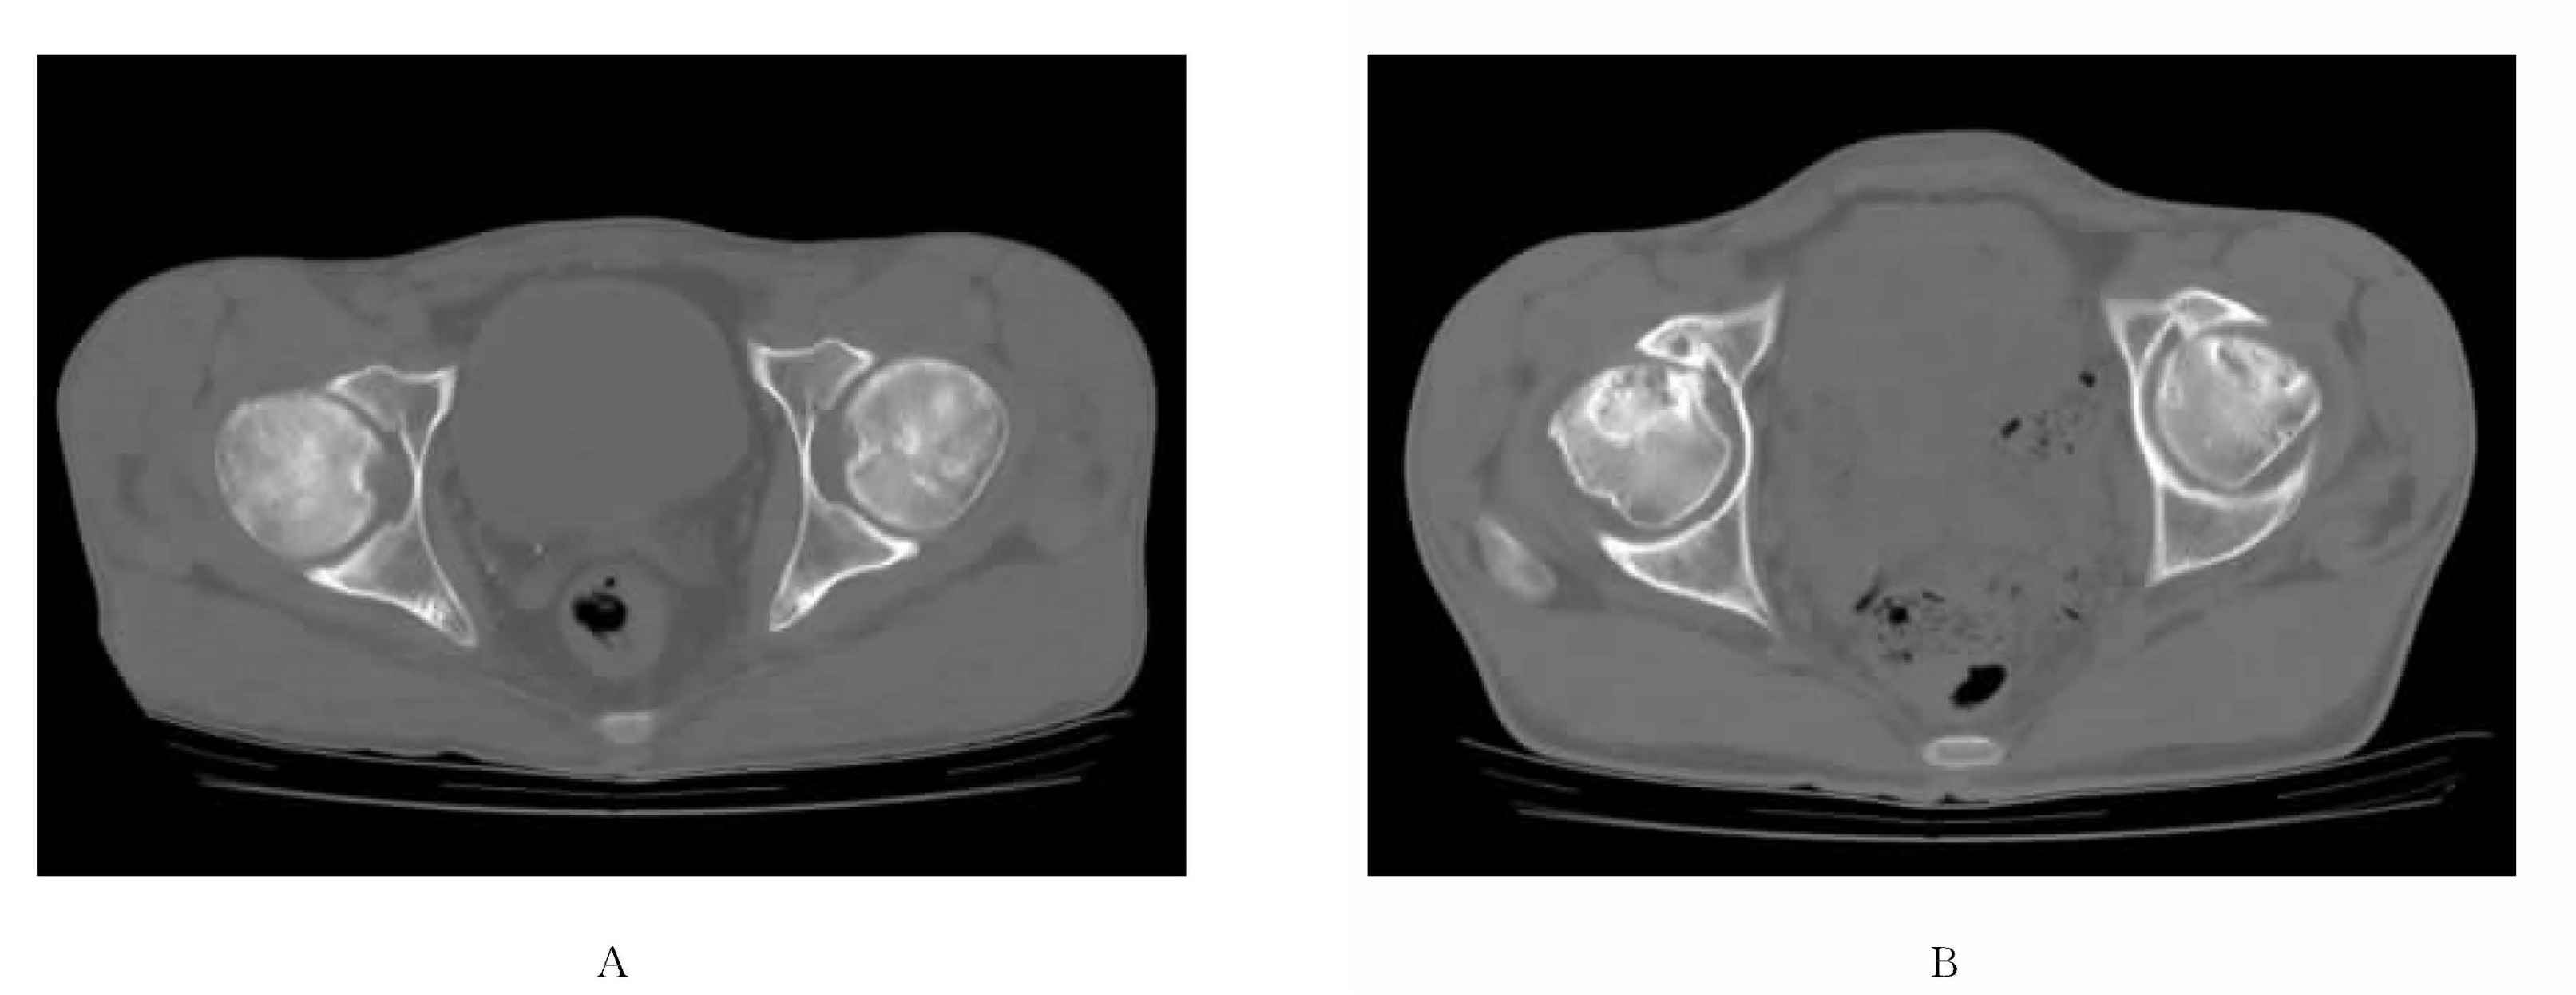
\includegraphics[width=.7\textwidth,height=\textheight,keepaspectratio]{./images/Image00462.jpg}
 \captionsetup{justification=centering}
 \caption{成人股骨头缺血坏死\\{\small A为早期坏死,可见双侧股骨头正常星芒状结构变形,股骨头内交织存在的簇状、条带状和斑片状高密度硬化区,边缘较模糊;B为中晚期坏死,可见双侧股骨头局限性轻度骨破碎、节裂、囊变和关节面微陷}}
 \label{fig22-36}
  \end{figure} 

5.缺血性髋关节病

国外有学者将成人股骨头缺血坏死分为骨型和骨软骨型,后者即缺血性髋关节病。它与骨型的最大区别是早期出现股骨头表面的软骨损害,故放射学兼有股骨头缺血坏死的早期表现和关节间隙变窄。本病软骨坏死所致的关节间隙变窄,并非继发退变所致。因股骨头缺血坏死的放射学表现尚处于早期,与晚期继发退变所致的关节间隙狭窄有别。本病晚期与骨型缺血坏死的放射学表现相同,同时应注意本病与髋臼缺血坏死非同一概念。

6.髂腰肌囊积液

髂腰肌囊又称髂耻囊、腰大肌囊,是髋关节周围最大、最恒定的滑囊,约98%的成人出现此囊,一般均为双侧。它位于髋关节前方、髂腰肌与耻骨肌之间,外侧为股直肌,内侧为股血管及股神经束。呈卵圆形,长5~7cm,宽2~4cm,平均为6cm×3cm。15%的髂腰肌囊与髋关节囊相通,在病理情况下可达30%~40%,交通口大小为0.1~3cm。而国内报道髂腰肌囊与髋关节囊相通者可达80%。

积液的病因:该囊积液扩张通常与先前存在的髋关节疾病如类风湿、化脓性感染、结核性滑膜炎、滑膜骨软骨瘤病、色素沉着绒毛结节性滑膜炎、股骨头缺血坏死、痛风、创伤等有关。以上因素可致髂腰肌囊滑膜充血、水肿、分泌增多,引起囊腔充盈扩张;滑膜受刺激增生,可引起滑膜囊壁增厚。髋关节囊积液膨胀,少数情况下可通过两者之间的开口进入髂腰肌囊内;多数情况下因髂腰肌腱的异常磨损而破裂,液体通过破裂口进入滑囊而扩张。

其CT表现为:①位于髋关节前方、股直肌内侧、股血管神经束的外侧、髂腰肌腱后方、耻骨肌前方的液性低密度影,增强扫描囊壁呈线样轻度强化。②股骨头中心层面以上多呈卵圆形,股骨头中心层面以下呈卵圆形或倒水滴状,可被肌束或纤维分隔成多囊状。③积液扩张的髂腰肌囊可沿髂腰肌扩展,上达腹股沟韧带上方进入盆腔;向下逐渐移向前内方,止于股骨小转子,偶见向下延伸至膝部。

7.影像学对股骨头缺血坏死预后的评估

国外有学者将股骨头受累程度分为3度:坏死范围<15%为轻度,坏死范围在15%~30%为中度,坏死范围>30%为重度。还有人用MR评估:坏死范围<25%的很少发生股骨头塌陷,范围>50%的病灶塌陷率增加。亦有人指出:病变位于内侧很少进展;病变居中,预后差;病变位于外侧面,预后最差。对本病的预后评估还有许多其他见解。

\textbf{【鉴别诊断】}
退行性髋关节病与股骨头缺血坏死尤其与骨软骨型常易混淆,应注意鉴别:①退行性髋关节病的破坏期以骨硬化和囊肿形成,骨性关节面变扁、变形为特点,且以持重部为著。囊变局限于关节面下,呈囊肿位于增厚骨小梁之间的表现。尤其无破碎、节裂征象有助于与缺血坏死相鉴别。②退行性变(包括其他关节的退行性变)亦可存在着不同程度的局部缺血坏死改变和表现,两者有不可分割的联系。且合并于退行性关节病的骨坏死表现,常被与退变有关的骨硬化和囊变所掩盖。另一方面,退行性关节病时骨端变扁和塌陷可能很明显,但不一定提示存在着明显的骨坏死。③股骨头缺血坏死的晚期需结合病史与退行性髋关节病的形成期相鉴别,影像学多难以鉴别。

退行性髋关节病常被误诊为股骨头缺血坏死,关键在于把股骨头囊变和关节面平直塌陷误为缺血坏死的特异性征象。

\subsection{膝关节骨坏死和自发性骨坏死}

1.膝关节骨坏死

发病率仅次于股骨头缺血坏死而居第2位,它是指发生于股骨远端和胫骨近端的膝关节周围骨坏死。发病原因有多种因素,可为继发性(外伤、激素治疗、酗酒、减压病、血液病等)或自发性(见下述),亦有原因不明者。

\textbf{【临床表现】} 多见于成年人,男女发病相近,多表现为膝关节疼痛。

\textbf{【影像学表现】}
早期多正常,随后可见骨小梁模糊、稀疏,软骨下低密度或混杂硬化。

2.膝关节自发性骨坏死

本病亦称为膝关节特发性骨坏死或原发性骨坏死,是上述膝关节骨坏死中的一种独立的临床疾病类型。其病因不明,骨质疏松、半月板损伤、骨性关节炎、肥胖或关节术后可能是其发病因素,还可见于胰腺炎病人。其病理改变类似于剥脱性骨软骨炎,晚期为继发性骨性关节炎。

\textbf{【临床表现】}
多见于50岁以上的患者,男女之比约1∶3。以突发性膝内侧痛为特点,症状可持续6~8周,以后逐渐缓解。患膝肿胀、积液,晚期关节持续肿胀、活动受限或关节绞锁。

\textbf{【影像学表现】}
病变可位于股骨髁、胫骨平台和髌骨。但90%位于股骨内髁的负重部关节软骨下,且多为一侧发病。病变在胫骨平台和负重相对较轻的股骨外髁少见,髌骨则更为少见。早期无特征性表现,2~4个月内可出现内髁变平、软骨下低密度区(负重区骨坏死),继而出现边缘硬化(修复带),受累髁部皮质增厚或骨膜反应。最终发展为继发性骨性关节炎。需注意与早期神经性关节病相鉴别。

\subsection{骨梗死}

本病又称为骨髓梗死、骨脂肪梗死,是指发生于干骺端、骨干的骨性坏死。发生于骨端的骨性坏死称为骨坏死。

\textbf{【病因病理】}
病因主要有老龄(多由于动脉粥样硬化)、镰状细胞贫血、潜水病、糖尿病、Gaucher病、Niemann-Pick病、感染、辐射、胰腺炎、血管炎及化学治疗等。其发生机理是局部的血液循环障碍所致。

病理:①急性期:局部血供中断,脂肪细胞发生胶样化和液化坏死,骨小梁细胞死亡,骨小梁结构尚存。②亚急性期:骨质吸收、反应性新骨形成和充血。③慢性期:坏死组织被肉芽组织和纤维组织替代而发生纤维化和营养不良性钙化、骨化。

\textbf{【临床表现】}
急性期有明显的局部疼痛、活动障碍。慢性期通常无症状,累及关节面可出现疼痛和畸形。

\textbf{【影像学表现】}
多发生于股骨下端、胫骨近端、肱骨上端及肱骨和桡骨下端等,可呈单发或多发性、对称或非对称性改变。病变范围大小不一,可为数毫米或延伸至骨干的大部。X线平片和CT表现如下:①急性期:不能发现或仅出现骨质疏松。②亚急性期:出现小的虫蚀样吸收和斑点状钙化。③慢性期:骨髓腔内不规则硬化斑块,排列成串或散在分布,呈蜿蜒走行的条状或地图样钙化(图\ref{fig22-37}),还可有骨膜增生和骨皮质增厚。

\begin{figure}[!htbp]
 \centering
 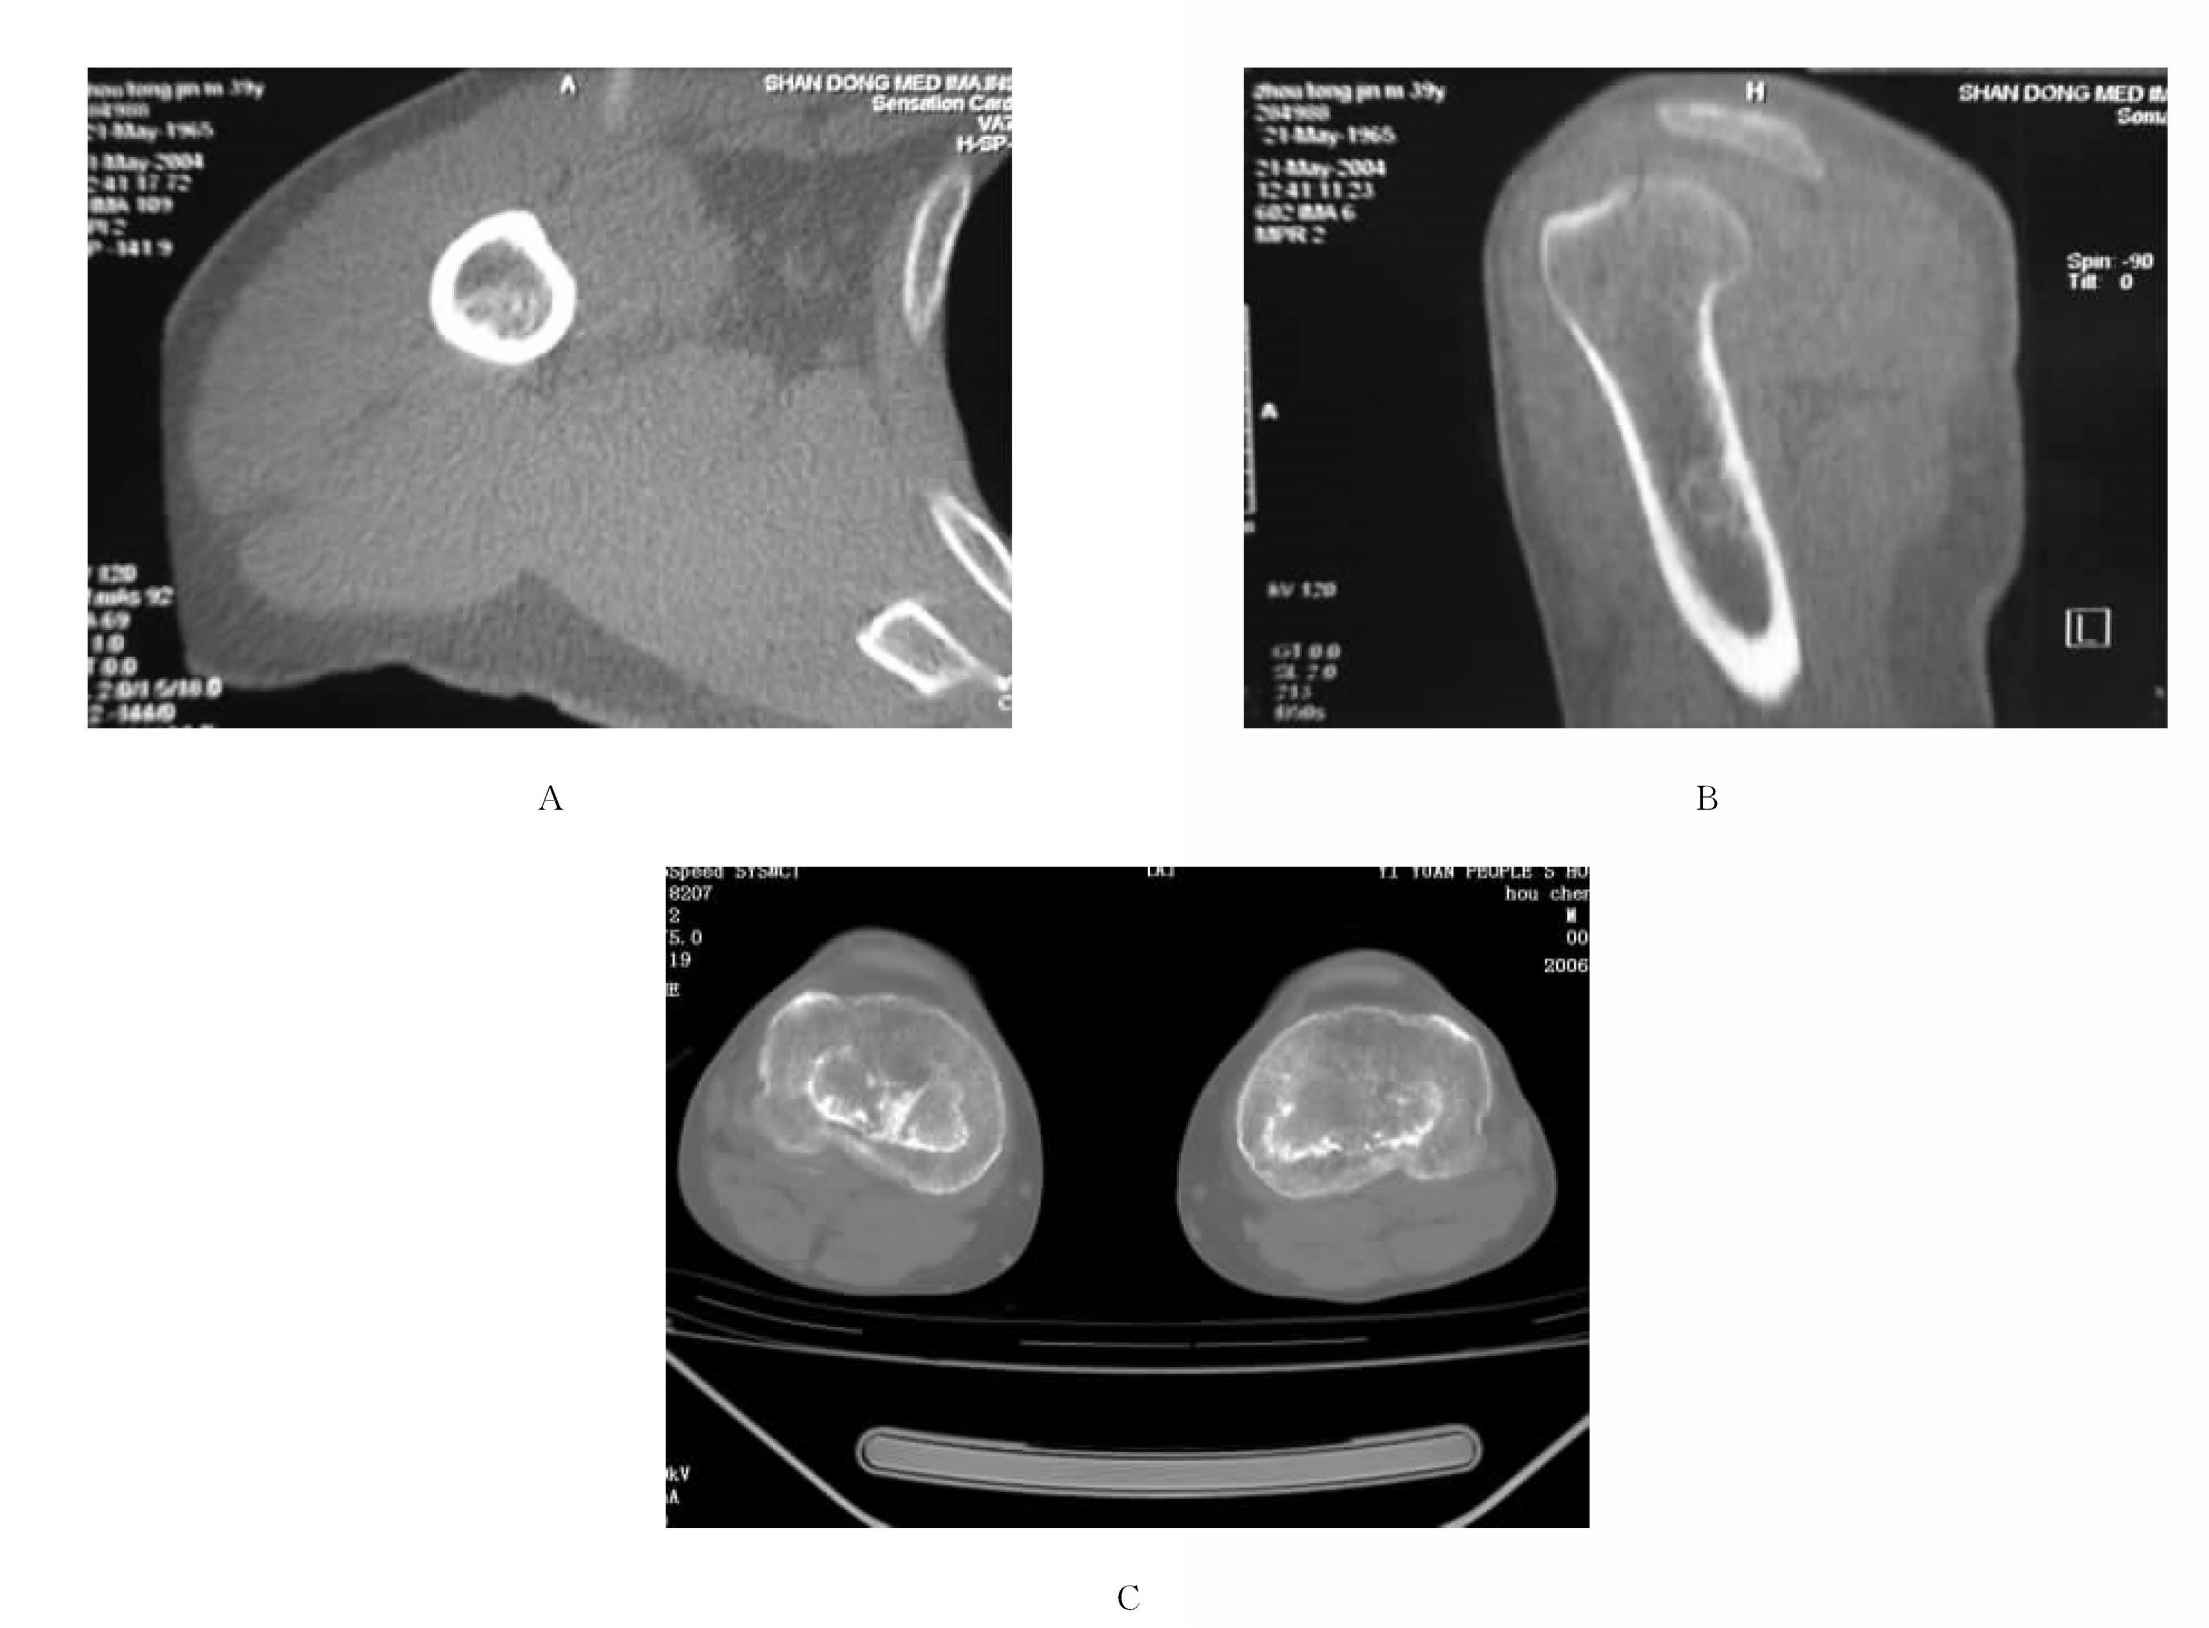
\includegraphics[width=.7\textwidth,height=\textheight,keepaspectratio]{./images/Image00463.jpg}
 \captionsetup{justification=centering}
 \caption{骨梗死\\{\small A、B为同一患者,示肱骨上段骨髓腔内不规则硬化斑块;C示双侧胫骨近端蜿蜒走行的地图样钙化}}
 \label{fig22-37}
  \end{figure} 

此外,骨梗死可继发感染和肿瘤应予注意。

\textbf{【鉴别诊断】}
局限性骨梗死应与纤维结构不良、内生软骨瘤、软骨肉瘤等鉴别。本病无弓状弯曲和髓腔膨胀,皮质不变薄,无软组织肿块和骨质破坏;梗死边缘性硬化带呈匍匐状或地图样,可资诊断和鉴别。

\protect\hypertarget{text00030.html}{}{}

